\documentclass[14pt]{extarticle}

% meta
\title{Отчет о практическом задании \\ <<Градиентные методы обучения линейных моделей. Применение линейных моделей для определения токсичности комментария>>.\\[6mm] \large Практикум 317 группы, ММП ВМК МГУ.}
\author{Булкин Антон Павлович.}
\date{Ноябрь 2024.}

\usepackage{hyperref}
\usepackage[warn]{mathtext}
\usepackage[T2A]{fontenc}			% кодировка
\usepackage[utf8]{inputenc}			% кодировка исходного текста
\usepackage[english,russian]{babel}	% локализация и переносы
\usepackage{indentfirst}
\usepackage{csquotes}
% \usepackage[bibstyle=gost-numeric, sorting=none]{biblatex}
% \addbibresource{biblio.bib}

% page settings
\usepackage[
    left=1.8cm,
    right=1.8cm,
    top=1.8cm,
    bottom=1.8cm,
    bindingoffset=0cm
]{geometry}

\usepackage{graphicx, hyperref, xcolor}
\hypersetup{
    colorlinks=true,
    linkcolor=teal,
    filecolor=magenta, 
    urlcolor=blue,
    citecolor=olive,
    pdftitle={GD},
    % pdfpagemode=FullScreen,
    linktoc=all
    }

\usepackage{wrapfig,caption}

% figures
\usepackage{caption}
\usepackage{subcaption}
\usepackage{floatrow}
\floatsetup{heightadjust=object}

% math
\usepackage{amsmath,amsfonts,amssymb,amsthm,mathtools,esint,eucal}

\begin{document}

\maketitle
\tableofcontents

\section{Вступление}

Данное задание посвящено ознакомлению с линейными моделями и градиентными методами обучения на примере задачи классификации токсичности комментария при помощи модели линейного классификатора. \\
Задачами задания являлись:
\begin{enumerate}
 \item Реализовать линейный классификатор с произвольной функцией потерь на языке Python без использования библиотеки \verb|scikit-learn|.
 \item Реализовать \textit{oracle}, использующий логистическую функцию потерь.
 \item Вывод необходимых формул и теоретических выкладок для понимания работы алгоритма.
 \item Выполнить 7 экспериментов на датасете токсичных комментариев в рамках решения задачи бинарной классификации.
 \item Провести предварительную обработку и преобразование выборки для упрощения решения задачи классификации.
\end{enumerate}

\section{Теоритическая часть}

\subsection{Формулы логистической регрессии}

Линейная модель классификации определяется как: $ a(x) = \text{sign}(\langle w, x \rangle + b), $ где \(w \in R^d\) — вектор весов, \(b \in R\) — сдвиг.

Величина $M_i(w, b)$ , называемая отступом объекта \( x_i \) относительно алгоритма \( a(x) \), определяется как: \( M_i(w, b) = y_i (\langle w, x_i \rangle + b) \).

Формула функции потерь логистической регрессии имеет вид: \\ $\mathcal{L}(M) = \log(1 + \exp(-M)) = \log(1 + \exp(-(\langle w, x \rangle + b)))$.

Тогда функция потерь выглядит: $Q(X, w) = \frac{1}{l} \sum_{i=1}^l \log\left(1 + e^{-y_i (w, x_i)}\right)$

\subsection{Вывод формулы градиента функции потерь для задачи бинарной логистической регрессии}
\[
\nabla_{w} Q(X, w) = \nabla_{w} \left( \frac{1}{l} \sum_{i=1}^l \log\left(1 + e^{-y_i (w,x_i)}\right) \right)
\]

Найдем производные по $w_j$:
\[
  \frac{\partial}{\partial w_j} (y_i (\langle w, x_i \rangle + b)) = y_i x_{ij}
\]

\[
\frac{\partial}{\partial w_j} L(w, x_i, b) = \frac{\partial}{\partial w_j} \left( \log \left( 1 + e^{-y_i (\langle w, x_i \rangle + b)} \right) \right) 
= \frac{-e^{-y_i (\langle w, x_i \rangle + b)}}{1 + e^{-y_i (\langle w, x_i \rangle + b)}} \cdot \frac{\partial}{\partial w_j} (y_i (\langle w, x_i \rangle + b))
\]

\[
\frac{\partial}{\partial w_j} Q(X, w) = \frac{\partial}{\partial w_j} \left( \frac{1}{l} \sum_{i=1}^l \log \left( 1 + e^{-y_i \langle w, x_i \rangle} \right) \right) = \frac{1}{l} \sum_{i=1}^l \left( y_i x_{ij} \right) \cdot \frac{-e^{-y_i \langle w, x_i \rangle}}{1 + e^{-y_i \langle w, x_i \rangle}} = \]
\[ 
= -\frac{1}{l} \sum_{i=1}^l \frac{y_i x_{ij}}{1 + e^{y_i (w, x_i)}}
\]

Следовательно, $\nabla_{w} Q(X, w) = -\frac{1}{l} \sum_{i=1}^l \frac{y_i x_i}{1 + e^{y_i \langle w, x_i \rangle}} $.

\subsection{Вывод формулы градиента функции потерь для задачи многоклассовой (мультиномиальной) логистической регрессии}

Функция потерь для задачи многоклассовой (мультиномиальной) логистической регрессии: \((w \in \mathbb{R}^{d \times K})\)
\[
L = -\frac{1}{l} \sum_{i=1}^l \ln P(y_i \mid x_i),
\]
где
$
P(y = j \mid x) = \frac{e^{\langle w_j x \rangle}}{\sum_{k=1}^K e^{ \langle w_k, x \rangle}}.
$

Посчитаем частные производные: $  \frac{\partial L}{\partial w_j} = -\frac{1}{l} \sum_{i=1}^l \frac{1}{P_i} \frac{\partial P_i}{\partial w_j} = -\frac{1}{l} \sum_{i=1}^l \frac{1}{P_i} \frac{\partial}{\partial w_j}(\frac{e^{\langle w_{y_i} x_i \rangle}}{\sum_{k=1}^K e^{ \langle w_k, x_i \rangle}}) = \ = -\frac{1}{l} \sum_{i=1}^l \frac{1}{P_i} (\frac{x_i e^{\langle w_j x_i \rangle} \sum_{k=1}^K e^{ \langle w_k, x_i \rangle} - e^{ \langle w_{y_i}, x_i \rangle} e^{ \langle w_j, x_i \rangle}} {(\sum_{k=1}^K e^{ \langle w_k, x_i \rangle})^2}) = -\frac{1}{l} \sum_{i=1}^l (x_i - x_i \cdot \frac{e^{ \langle w_j, x_i \rangle}}{\sum_{k=1}^K e^{ \langle w_k, x_i \rangle}}) = \\ = -\frac{1}{l} \sum_{i=1}^l (x_i - P(y = j \mid x_i) \cdot x_i)
$



\section{Обработка данных}

\subsection{Предварительная обработка текста}

Проведем предварительную обработку текста комментариев:
\begin{enumerate}
    \item Приведем все тексты к нижнему регистру при помощи \textit{str.lower()}
    \item Заменим все символы, не являющиеся цифрами или буквами, на пробелы
\end{enumerate}

\subsection{Преобразование выборки}

Проведем преобразование выборки в разреженную матрицу \textit{scipy.sparse.csr\_matrix}, где значению в \textit{\((i, j)\)} позиции соответствует число встреченных слов \textit{j} в документе \textit{i}, при помощи \textit{sklearn.feature\_extraction.text.CountVectorizer}, который реализует модель представления текста \textit{Bag of Words}, в которой каждый текстовый документ представляется вектором, который отражает частоты слов, присутствующих в документе. Столбцы вектора соответствуют уникальным словам из всего корпуса документов. При применении \textit{CountVectorizer} укажем параметр \textit{min\_df}, равный 0.001, чтобы уменьшить размерность данных и ускорить проведение экспериментов.

\section{Сравнение численного подсчета градиента функции потерь с вычислением по аналитической формуле}

\subsection{Постановка задачи}

Сравните численный подсчет градиента функции потерь из модуля utils.py с вычислением по аналитической формуле.

\subsection{Реализация}
Для сравнения алгоритмов подсчета градиента функции потерь сгенерируем выборки размера \textit{\((500000, x)\)}, где \textit{\( x \in \{5, 25, 75, 100, 125, 175, 250, 350, 500, 1000\} \)}, чтобы сравнить работу алгоритмов на данных с разными размерами признакового пространства.

На рисунках \hyperref[fig:testic]{1} и \hyperref[fig:exp_3_rmse_dim]{2} представлены графики зависимости времени работы алгоритмов и значения RMSE (евклидовой нормы вектора разности результатов работы алгоритмов, деленной на \(\sqrt{n}\)) от размерности признакового пространства выборки.

\begin{figure}[H]
    \centering
    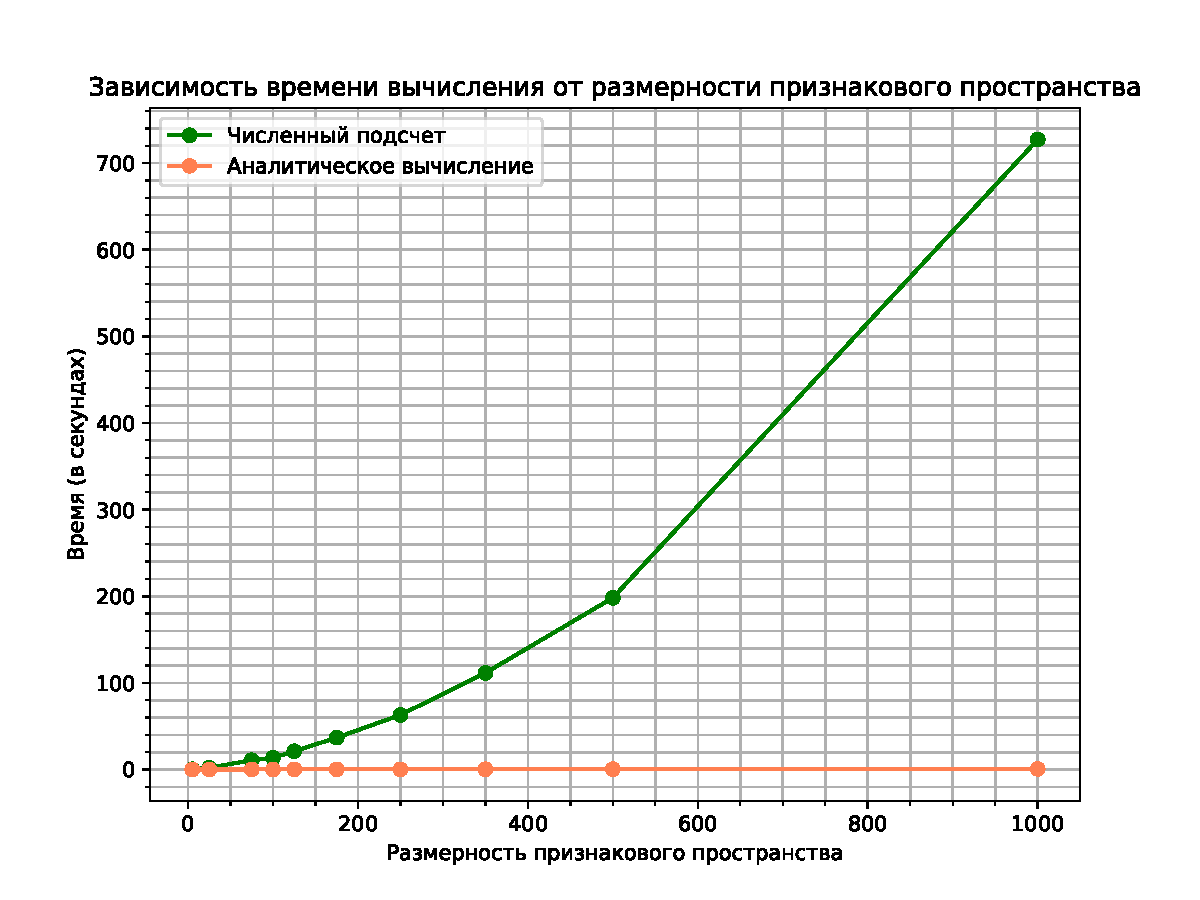
\includegraphics[width=0.65\linewidth]
    {exp_3_time_dim.pdf}
    \caption{Время работы алгоритмов подсчета градиента функции в зависимости от размера признакового пространства}
    \label{fig:testic}
\end{figure}

\begin{figure}[H]
    \centering
    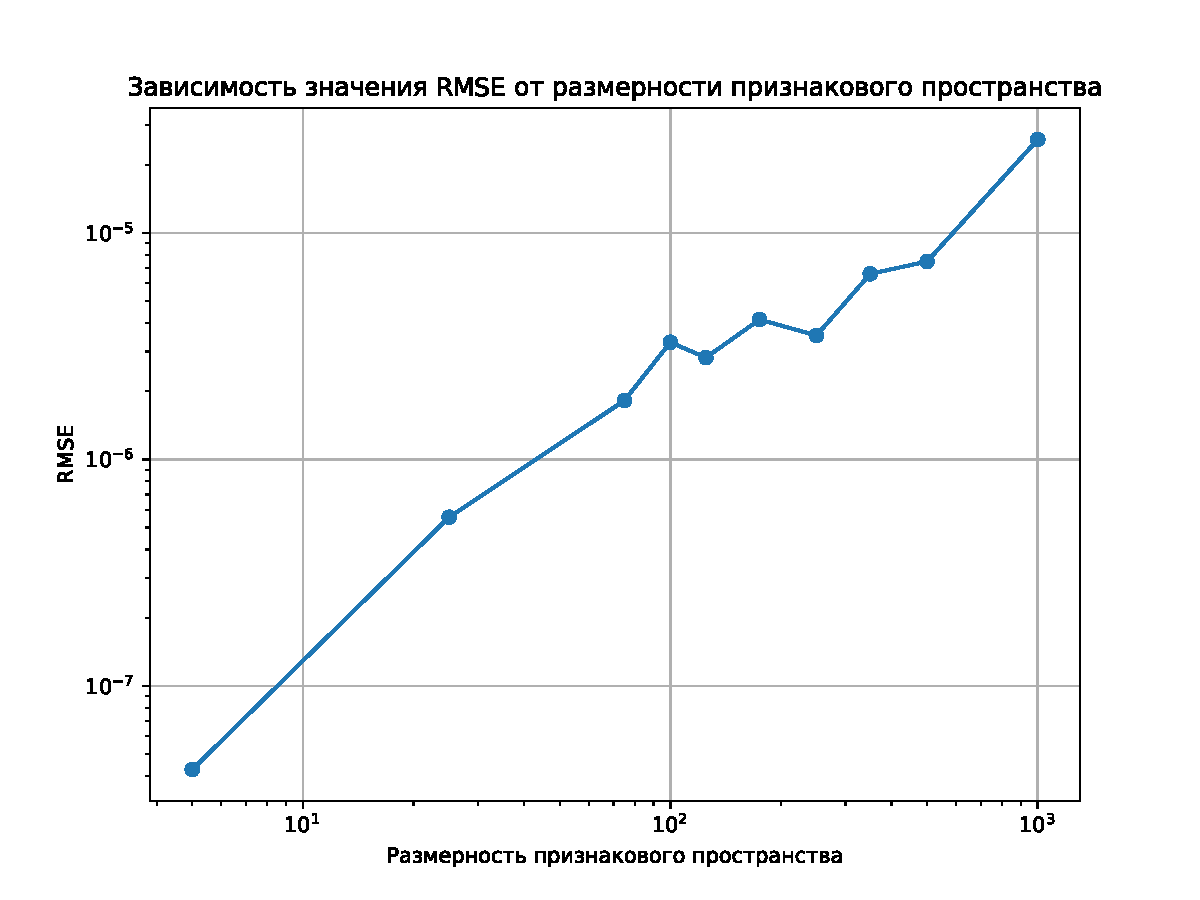
\includegraphics[width=0.65\linewidth]
    {exp_3_rmse_dim.pdf}
    \caption{Значение RMSE в зависимости от размера признакового пространства}
    \label{fig:exp_3_rmse_dim}
\end{figure}

При сравнении аналитического и численного вычисления градиента функции потерь использовался лосс для бинарной логистической задачи классификации (\textit{Binary Log-Loss}), т.е. $ Q(X, w) = \frac{1}{l} \sum_{i=1}^{l} \log\left(1 + e^{y_i <\mathbf{w}, \mathbf{x}_i>}\right ) + \frac{\lambda}{2} \|\mathbf{w}\|_2^2 $.

Аналитический метод подсчета градиента выполнялся по формуле: \\ $ \nabla_{\mathbf{w}} Q(\mathbf{X}, \mathbf{w}) = -\frac{1}{N} \sum_{i=1}^{N} \mathbf{x}_i \cdot y_i \cdot \sigma\left(-y_i \cdot (\mathbf{w}^\top \mathbf{x}_i)\right) + \lambda \mathbf{w} $

Численный же метод подсчета градиента представлял собой: \\
$ \nabla_{\mathbf{w}} Q(X, w) = \left( \frac{\partial}{\partial w_0},
\frac{\partial}{\partial w_1}, \ldots, \frac{\partial}{\partial w_l} \right), \\ $ где $ \ \frac{\partial}{\partial w_j} = \frac{Q(X, w + \epsilon * \mathbf{e}_j) - Q(X, w)}{\epsilon}, \
e_{ij} = \begin{cases} 1, & \text{если } i = j, \\ 0, & \text{если } i \neq j, \end{cases} \quad \epsilon = 10^{-8}. $

\subsection{Выводы}

Исследование показало, что алгоритм численного подсчета лишь немного уступает аналитическому методу в вычислении градиента функции потерь, так как значение RMSE методов почти не превосходит $ 10^{-5} $.

Однако, как можно заметить из графиков, время вычисления градиента функции потерь значительно растет с ростом размерности признакового пространства, в отличие от аналитического метода вычисления, скорость выполнения которого практически не изменяется с ростом размерности признакового пространства.

Из перечисленного выше, можно сделать вывод, что аналитический метод работает эффективнее по времени, поэтому в дальнейшим будем использовать его.

\section{Исследование поведения градиентного спуска для задачи логистической регрессии в зависимости от \textit{step\_alpha}, \textit{step\_beta} и начального приближения} \label{sec:section5}

\subsection{Постановка задачи}

Исследовать поведение градиентного спуска для задачи логистической регрессии в зависимости от следующих параметров:
\begin{itemize}
    \item параметр размера шага \texttt{step\_alpha}
    \item параметр размера шага \texttt{step\_beta}
    \item начального приближения
\end{itemize}

Исследование поведения метода подразумевало анализ следующих зависимостей:
\begin{itemize}
    \item зависимость значения функции потерь от итерации метода
    \item зависимость точности (accuracy) итерации метода
\end{itemize}

\subsection{Реализация}

Во всех экспериментах до подбора наилучшего параметра при прочих равных увсловиях брались как тестирующие значения параметры:
\begin{itemize}
    \item \textit{step\_beta = 0}
    \item \textit{l2\_coef = 0.001}
    \item \textit{max\_iter = 1000}
\end{itemize}

После нахождения наилучшего параметра - использовался он.

\subsubsection{Подбор параметра \textit{step\_alpha}}

Будем рассматривать значения \textit{step\_alpha}, равномерно расположенные по логарифмической шкале от $ 10^{-4} $ до 10.

\begin{figure}[H]
    \centering
    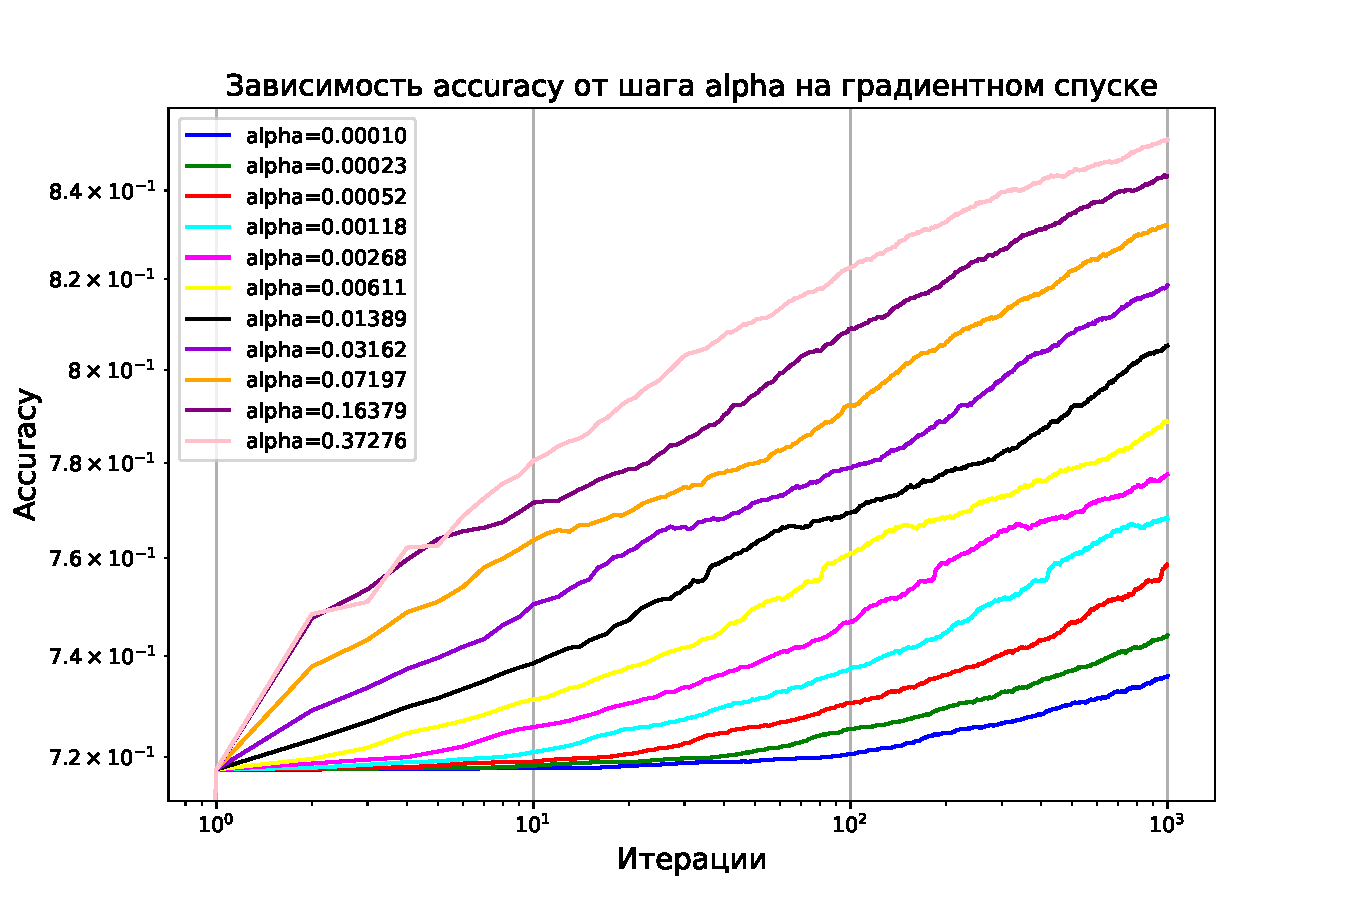
\includegraphics[width=0.7\linewidth]
    {exp_4_acc_alpha_1.pdf}
    \caption{Accuracy на итерациях модели в зависимости от параметра \textit{step\_alpha}}
    \label{fig:exp_4_acc_alpha_1}
\end{figure}

\begin{figure}[H]
    \centering
    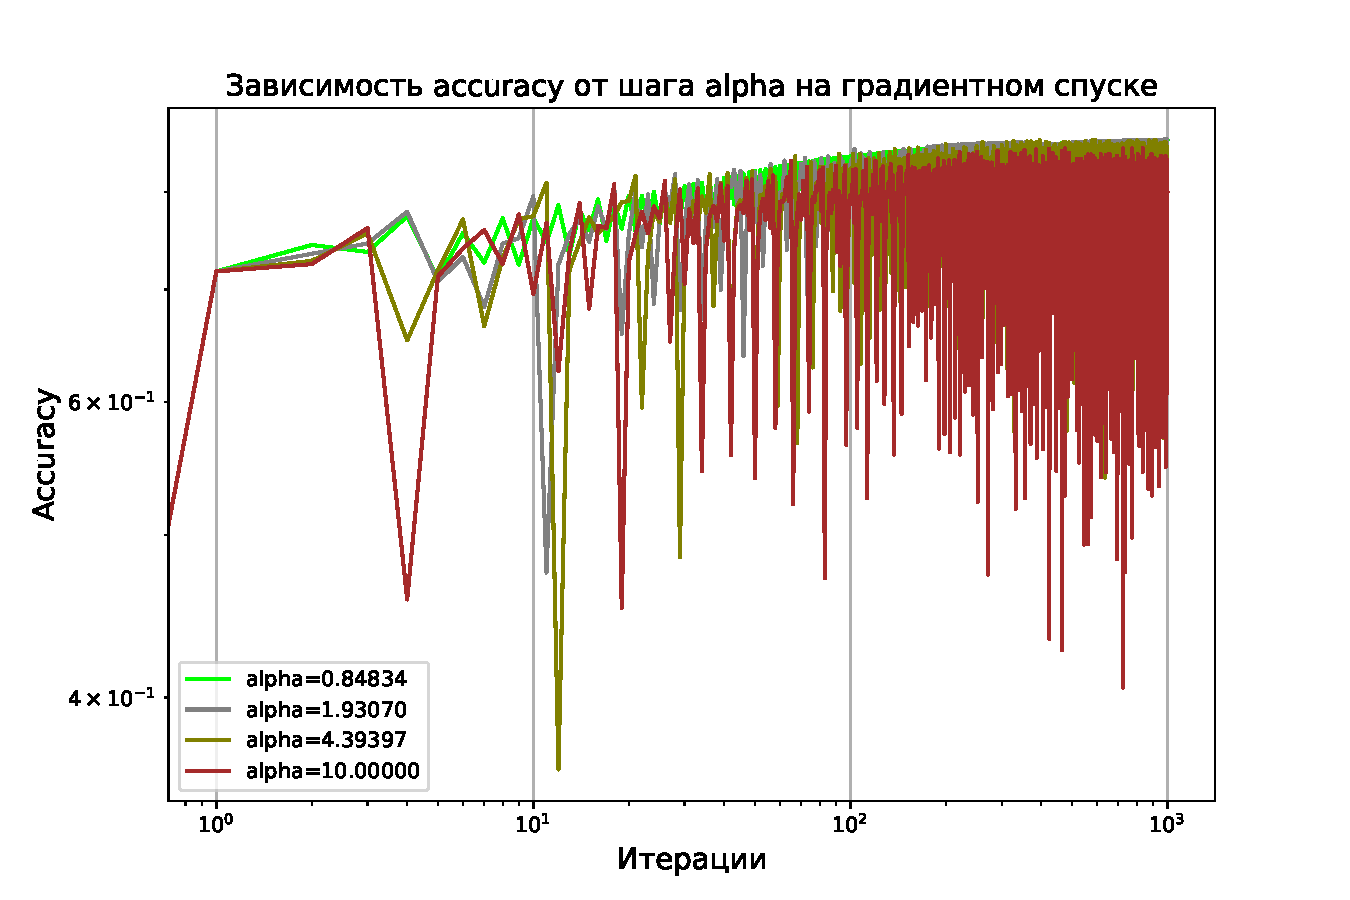
\includegraphics[width=0.7\linewidth]
    {exp_4_acc_alpha_2.pdf}
    \caption{Accuracy на итерациях модели в зависимости от параметра \textit{step\_alpha}}
    \label{fig:exp_4_acc_alpha_2}
\end{figure}

На рисунках \hyperref[fig:exp_4_acc_alpha_1]{3} и \hyperref[fig:exp_4_acc_alpha_2]{4} представлены графики зависимости accuracy модели на каждой итерации градиентного спуска от параметра \textit{step\_alpha}. Как можно заметить из графиков, наилучшая точность модели достигается при \textit{step\_alpha = 0.372759372}.

\begin{figure}[H]
    \centering
    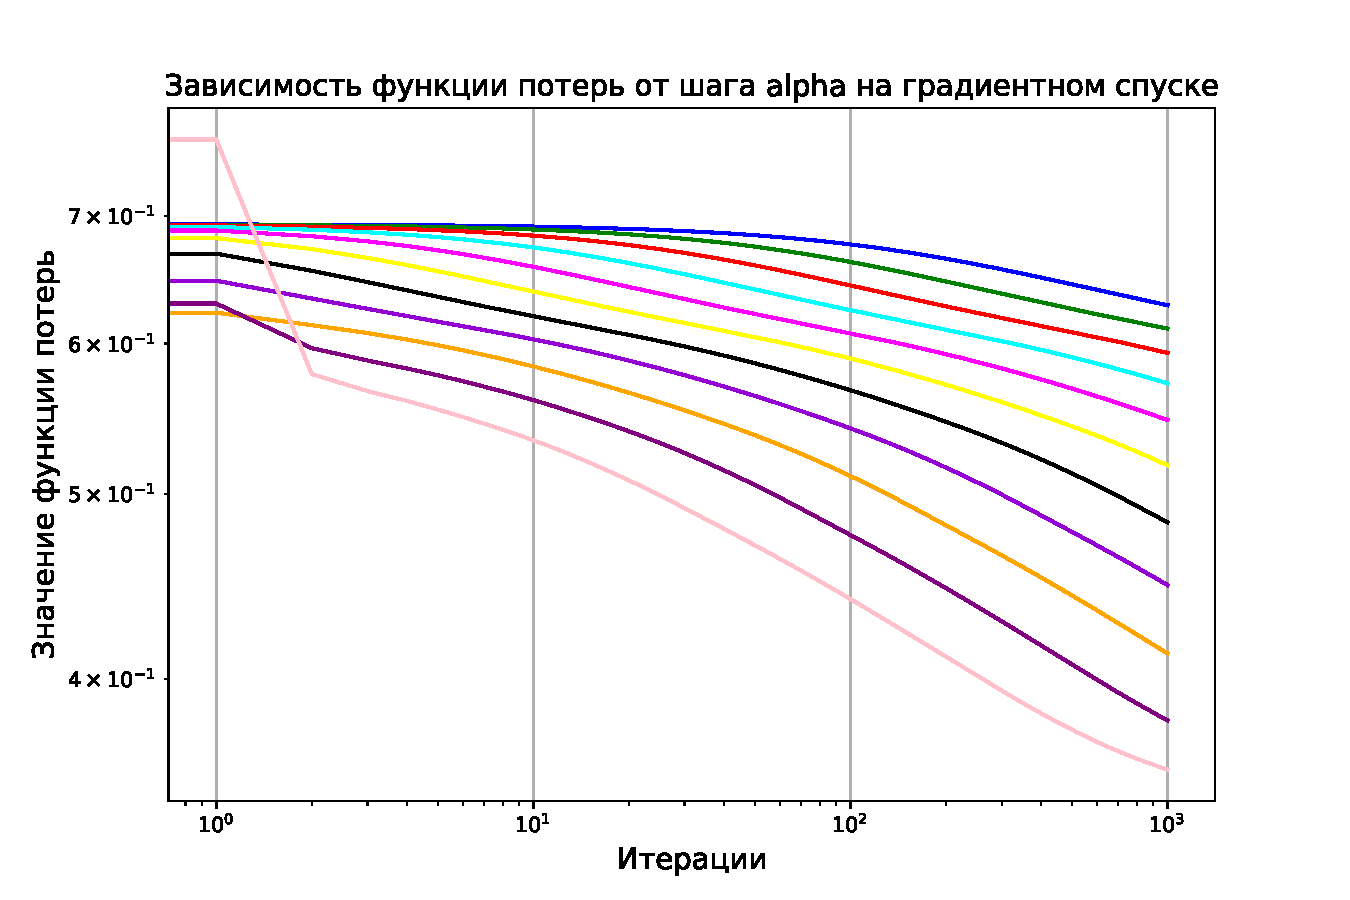
\includegraphics[width=0.7\linewidth]
    {exp_4_loss_alpha_1.pdf}
    \caption{Значение функции потерь на итерациях модели в зависимости от параметра \textit{step\_alpha}}
    \label{fig:exp_4_loss_alpha_1}
\end{figure}

\begin{figure}[H]
    \centering
    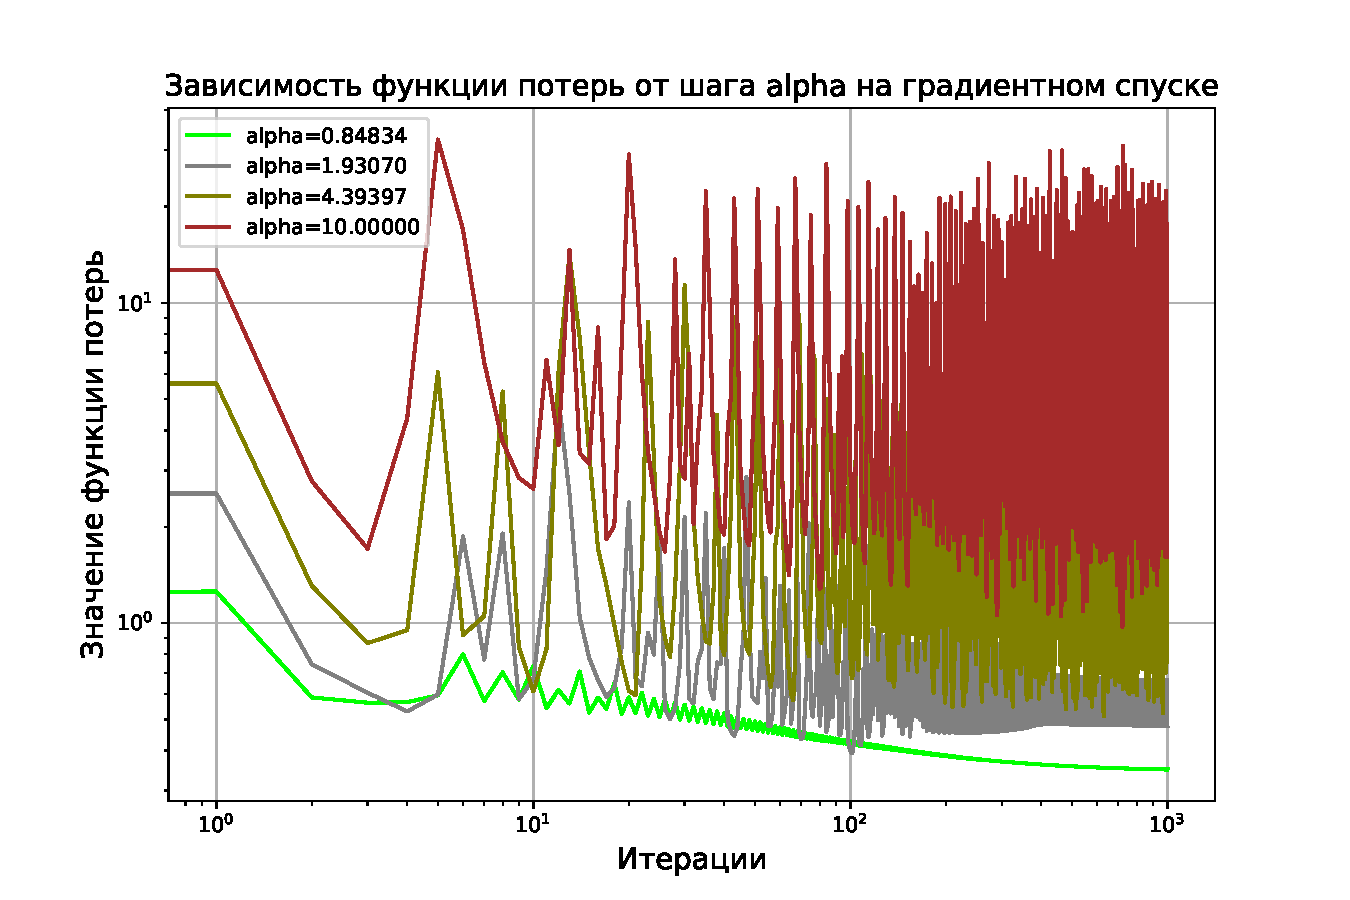
\includegraphics[width=0.7\linewidth]
    {exp_4_loss_alpha_2.pdf}
    \caption{Значение функции потерь на итерациях модели в зависимости от параметра \textit{step\_alpha}}
    \label{fig:exp_4_loss_alpha_2}
\end{figure}

На рисунках \hyperref[fig:exp_4_loss_alpha_1]{5} и \hyperref[fig:exp_4_loss_alpha_2]{6} представлены графики зависимости значения функции потерь на каждой итерации градиентного спуска от параметра \textit{step\_alpha}. Как можно заметить из графиков, наилучшая сходимость значений функции потерь модели достигается при \textit{step\_alpha = 0.372759372}.

\subsubsection{Подбор параметра \textit{step\_beta}}

Будем рассматривать значения \textit{step\_beta} среди следующего множества значений: \( \{0, \ 0.0001, \ 0.001, \ 0.005, \ 0.01, \ 0.05, \ 0.1, \ 0.2, \ 0.3, \ 0.5, \ 0.7, \ 1, \ 2, \ 3, \ 4, \ 5, \ 10, \ 15, \\ 25, \ 50, \ 75, \ 100\} \).

\begin{figure}[H]
    \centering
    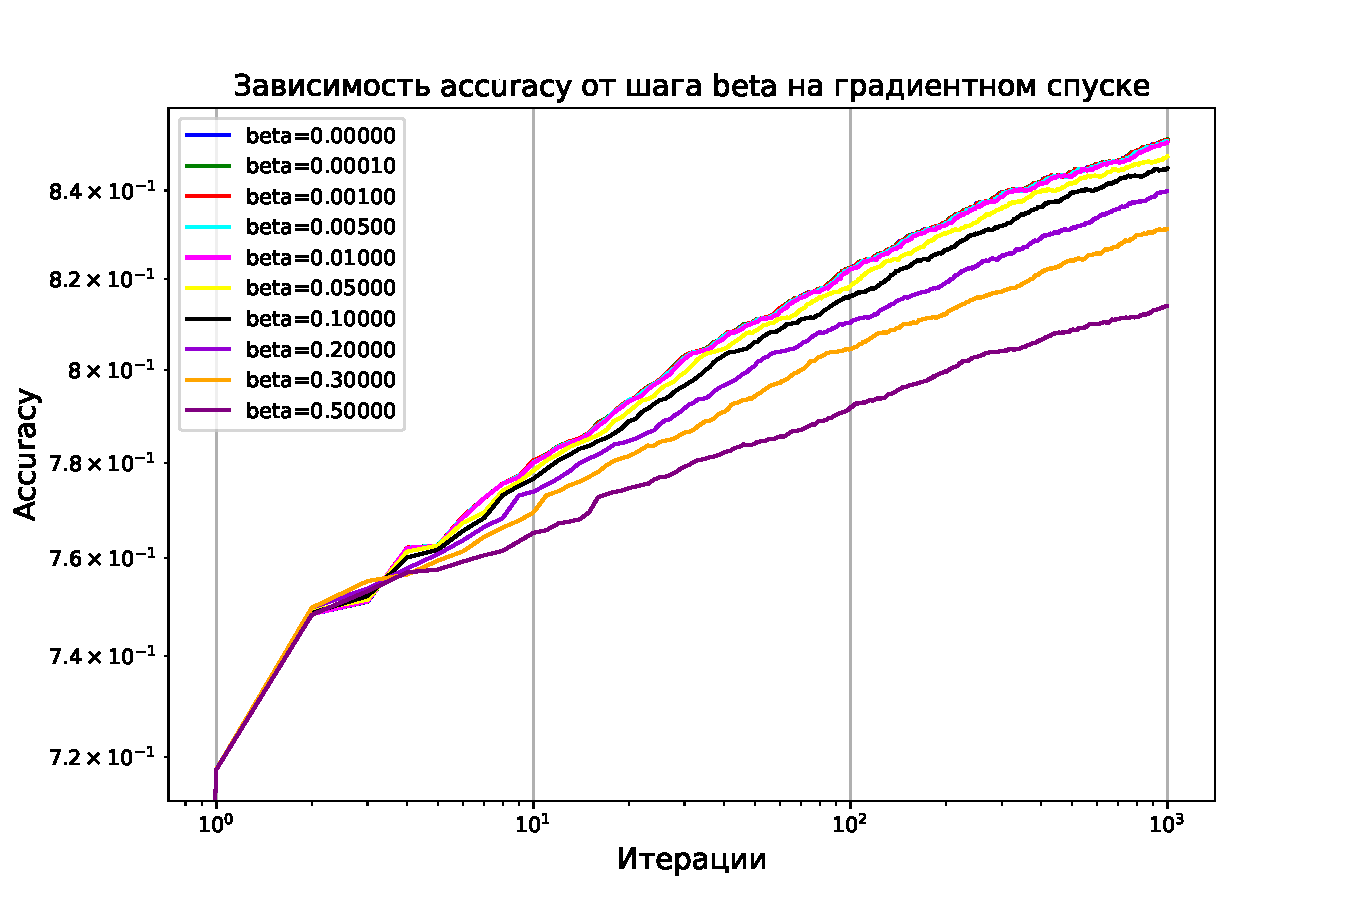
\includegraphics[width=0.7\linewidth]
    {exp_4_acc_beta_1.pdf}
    \caption{Accuracy на итерациях модели в зависимости от параметра \textit{step\_beta}}
    \label{fig:exp_4_acc_beta_1}
\end{figure}

\begin{figure}[H]
    \centering
    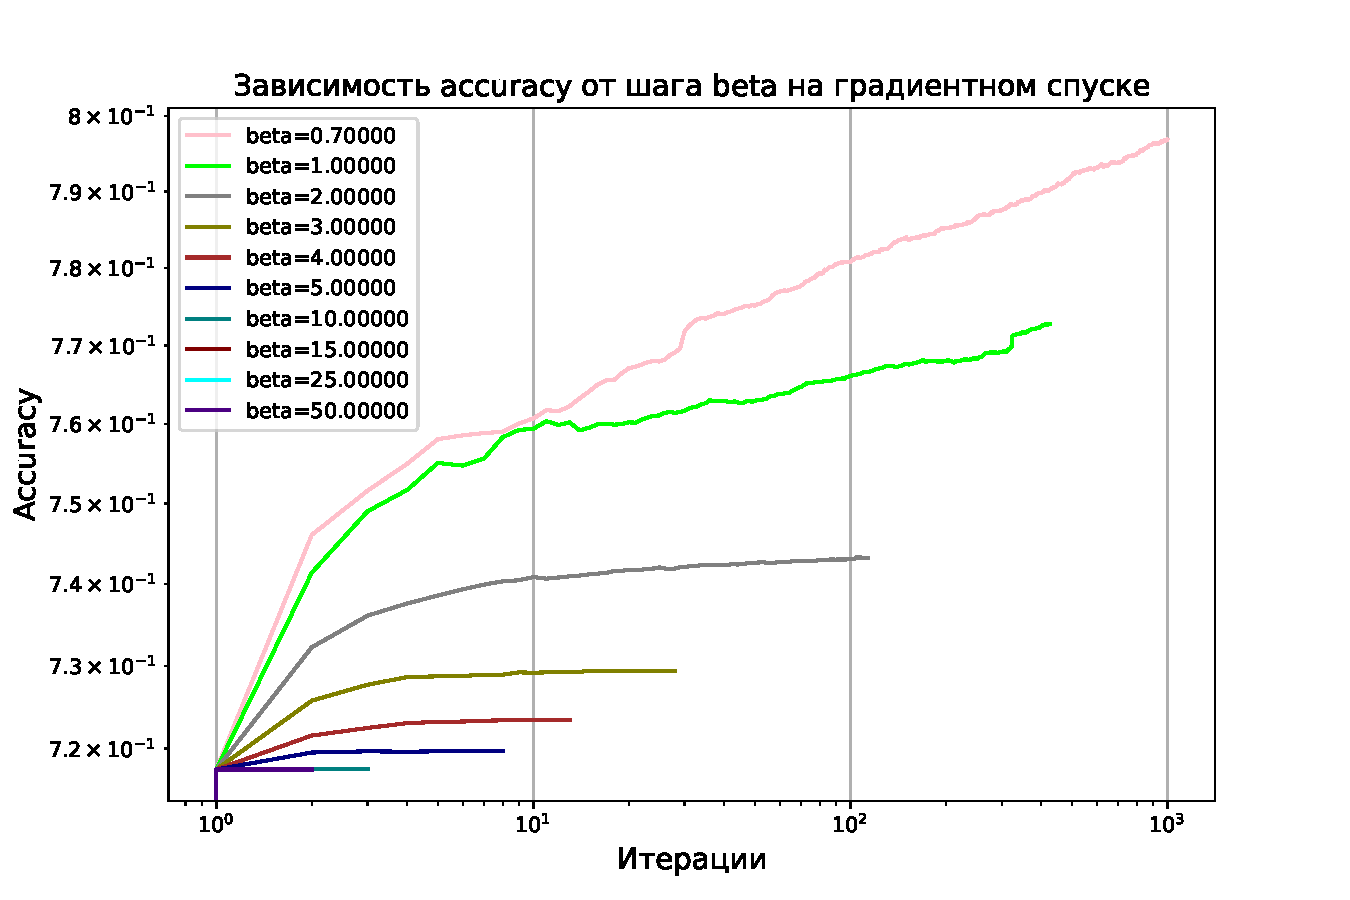
\includegraphics[width=0.7\linewidth]
    {exp_4_acc_beta_2.pdf}
    \caption{Accuracy на итерациях модели в зависимости от параметра \textit{step\_beta}}
    \label{fig:exp_4_acc_beta_2}
\end{figure}

На рисунках \hyperref[fig:exp_4_acc_beta_1]{7} и \hyperref[fig:exp_4_acc_beta_2]{8} представлены графики зависимости accuracy модели на каждой итерации градиентного спуска от параметра \textit{step\_beta}. Как можно заметить из графиков, наилучшая точность модели достигается при \textit{step\_beta = 0}.

Также можно заметить, что часть графиков на рисунке \hyperref[fig:exp_4_acc_beta_2]{8} имеют отличный характер зависимости от других, так как алгоритм градиентного спуска заканчивается раньше, чем проходит все итерации, так как модуль разницы последовательных на итерациях значений функции потерь становится меньше, чем \textit{tolerance}, что приводит к остановке алгоритма.

\begin{figure}[H]
    \centering
    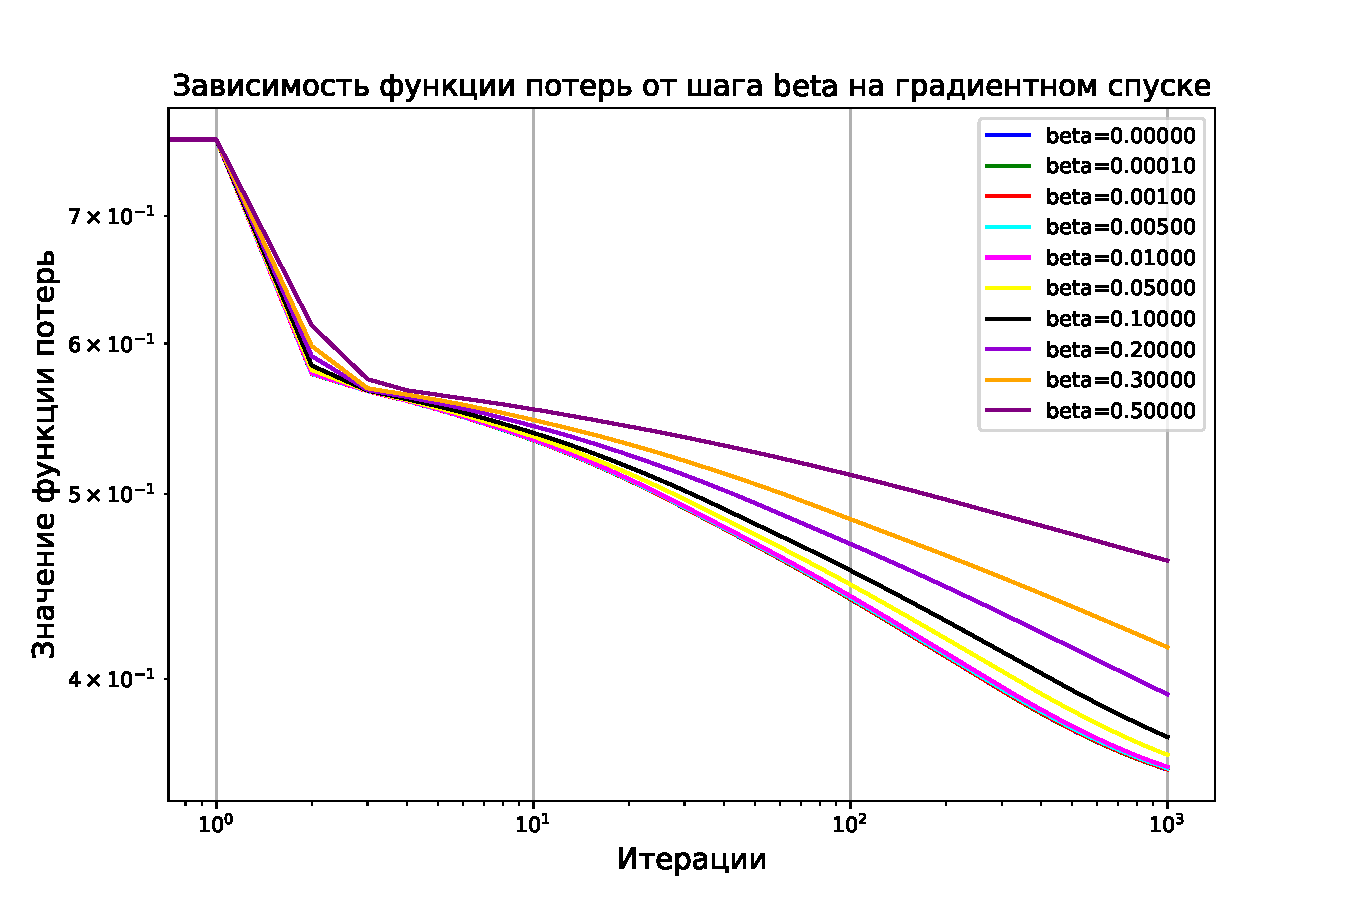
\includegraphics[width=0.7\linewidth]
    {exp_4_loss_beta_1.pdf}
    \caption{Значение функции потерь на итерациях модели в зависимости от параметра \textit{step\_beta}}
    \label{fig:exp_4_loss_beta_1}
\end{figure}

\begin{figure}[H]
    \centering
    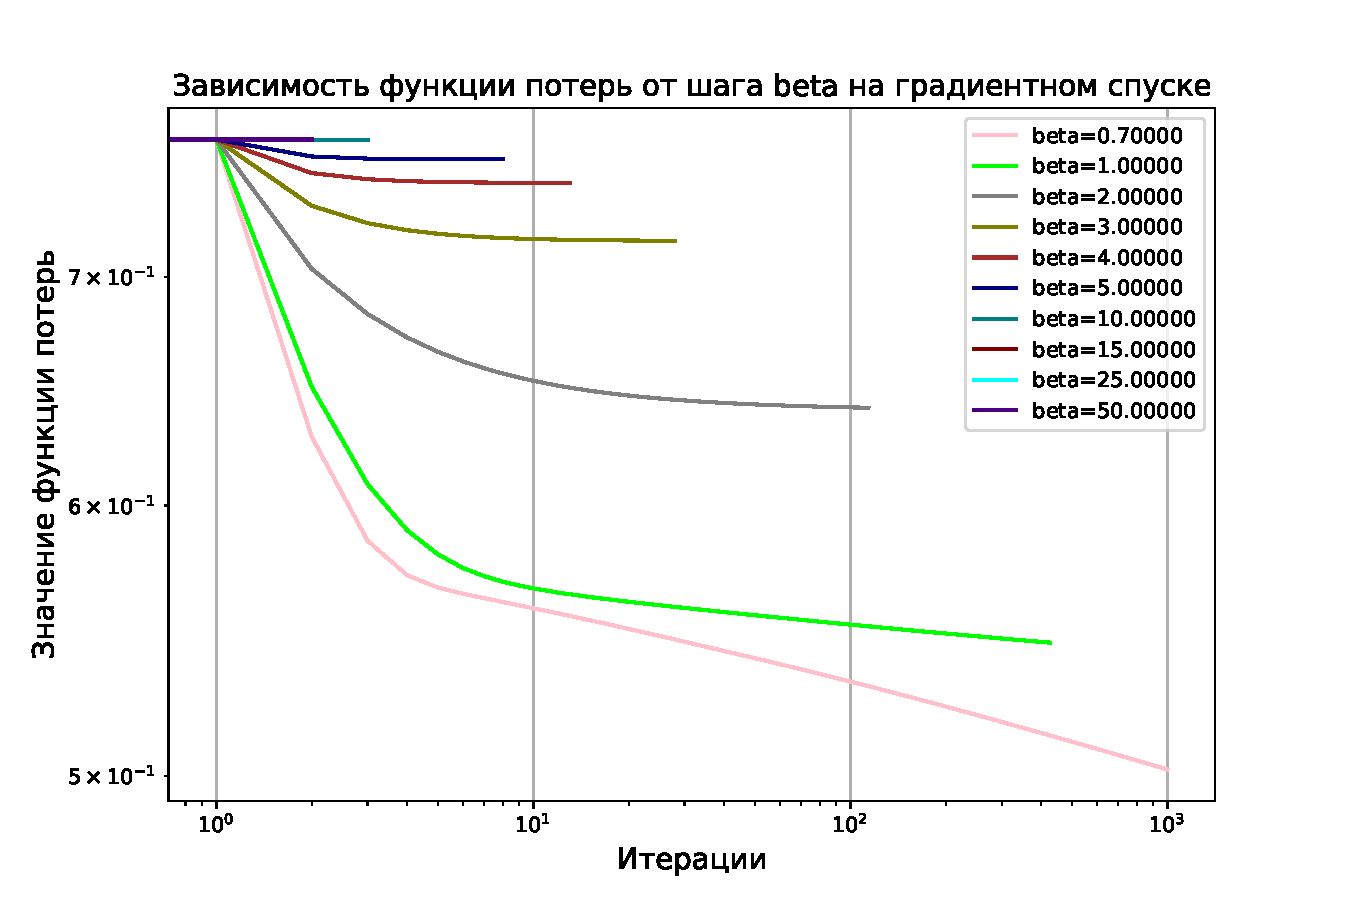
\includegraphics[width=0.7\linewidth]
    {exp_4_loss_beta_2.pdf}
    \caption{Значение функции потерь на итерациях модели в зависимости от параметра \textit{step\_beta}}
    \label{fig:exp_4_loss_beta_2}
\end{figure}

На рисунках \hyperref[fig:exp_4_loss_beta_1]{9} и \hyperref[fig:exp_4_loss_beta_2]{10} представлены графики зависимости значения функции потерь на каждой итерации градиентного спуска от параметра \textit{step\_beta}. Как можно заметить из графиков, наилучшая сходимость значений функции потерь модели достигается при \textit{step\_beta = 0}, причём алгоритм проходит все итерации, а точность (accuracy) оказывается выше, чем при других значениях \textit{step\_beta}.

\subsubsection{Подбор начального приближения весов \textit{$ w_0 $}}

Будем рассматривать значения начального приближения весов \textit{$ w_0 $}, используя функции \textit{Numpy}, такие как \textit{np.random.normal} и \textit{np.random.uniform}, соответствующие нормальному и равномерному распределениям. Рассмотрим значения начального приближения весов, соответствующие данным распределениям со следующими параметрами:
\begin{itemize}
    \item normal 0, 0.1
    \item normal 0, 0.25
    \item normal 0, 0.5
    \item normal 0, 0.75
    \item normal 0, 1
    \item uniform -0.1, 0.1
    \item uniform -0.5, 0.5
    \item uniform -1, 1
    \item uniform -2, 2
    \item uniform -5, 5
    \item uniform -10, 10
    \item uniform -50, 50
\end{itemize}

А также начальное приближение весов: нулями и по формуле: $ w_j = \frac{\langle f_j, y
\rangle}{\langle f_j, f_j \rangle}, \\ \text{где } y \text{ — вектор меток, } f_j
\text{ — столбец признака, а }  w_j \text{ - } j \text{-й элемент вектора весов } w_0$

\begin{figure}[H]
    \centering
    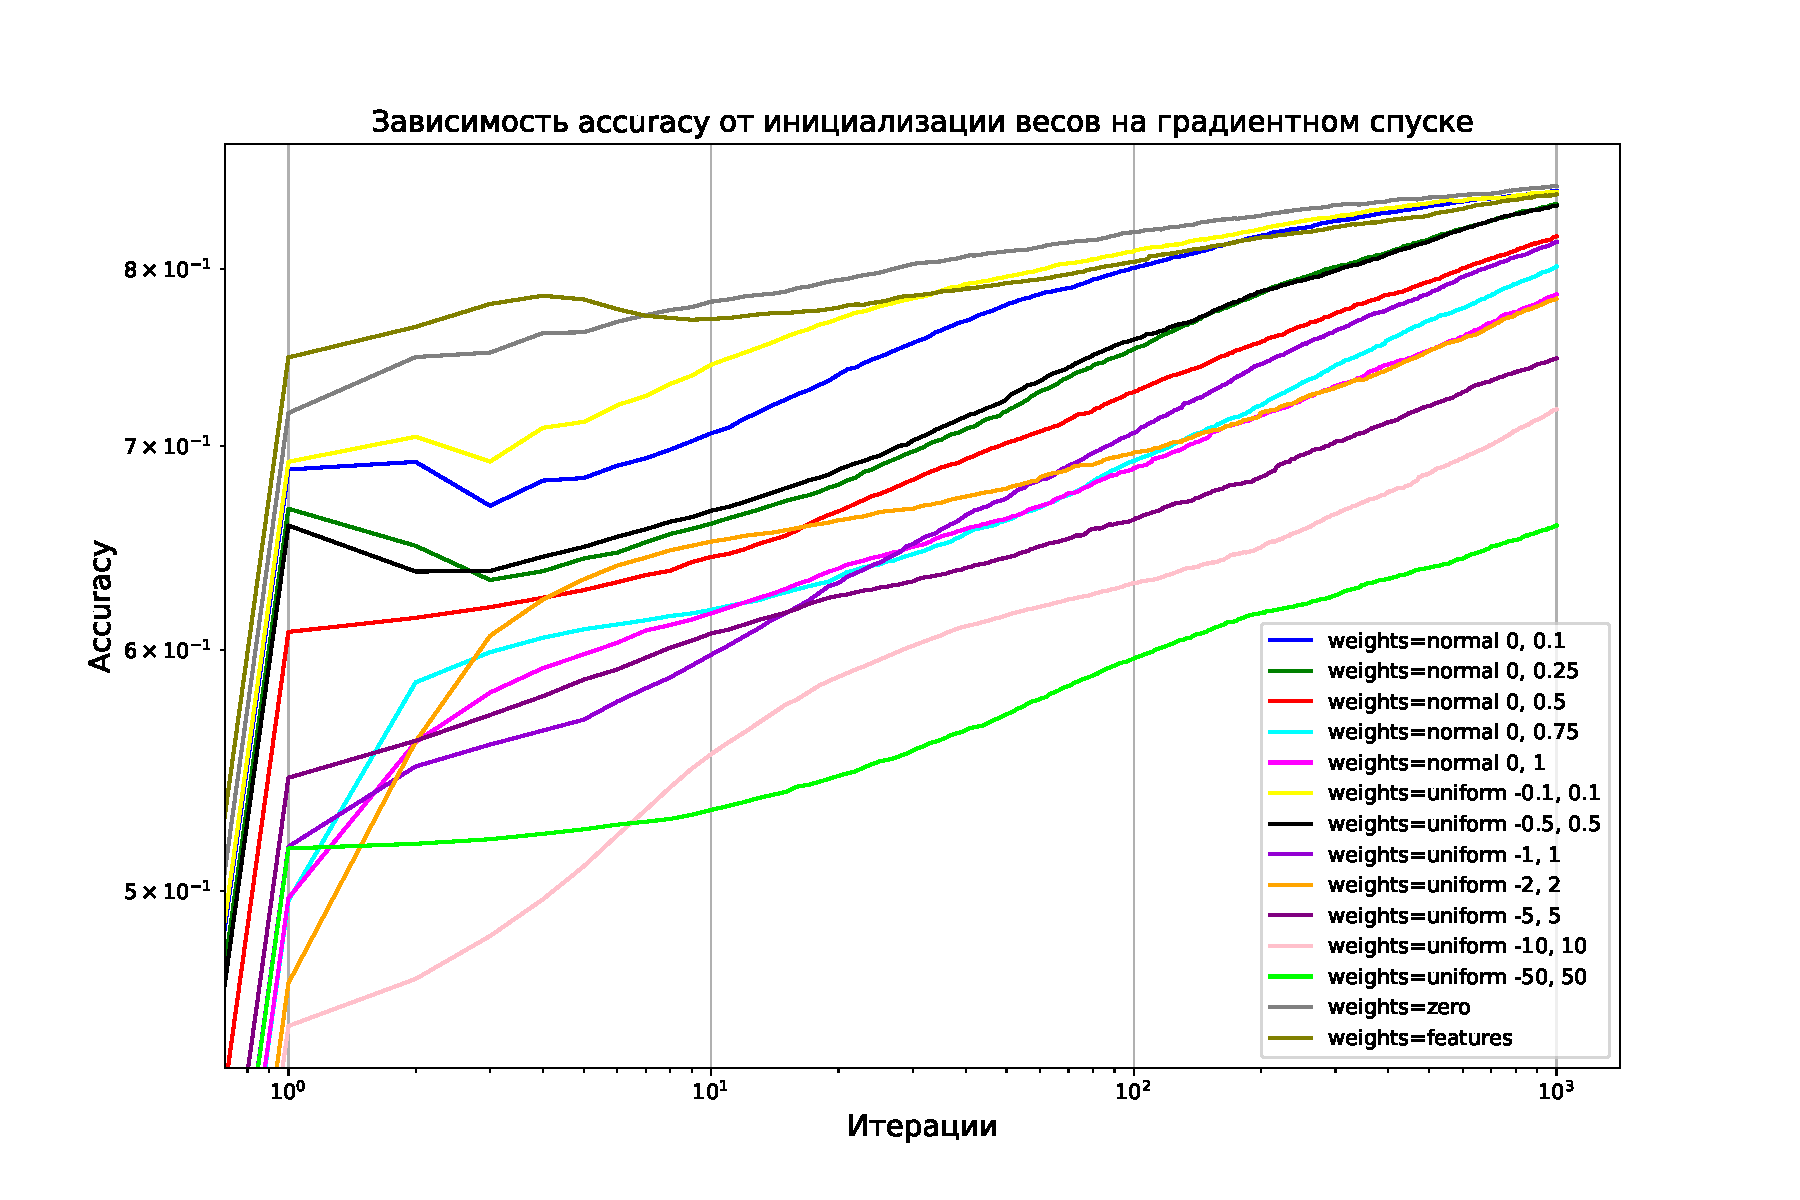
\includegraphics[width=1\linewidth]
    {exp_4_acc_weights.pdf}
    \caption{Accuracy на итерациях модели в зависимости от начального приближения весов}
    \label{fig:exp_4_acc_weights}
\end{figure}

На рисунке \hyperref[fig:exp_4_acc_alpha_1]{11} представлены графики зависимости accuracy модели на каждой итерации градиентного спуска от начального приближения весов \textit{$ w_0 $}. Как можно заметить из графиков, наилучшая точность модели достигается при \textit{$ w_0 = (0, ... , 0)$}.

\begin{figure}[H]
    \centering
    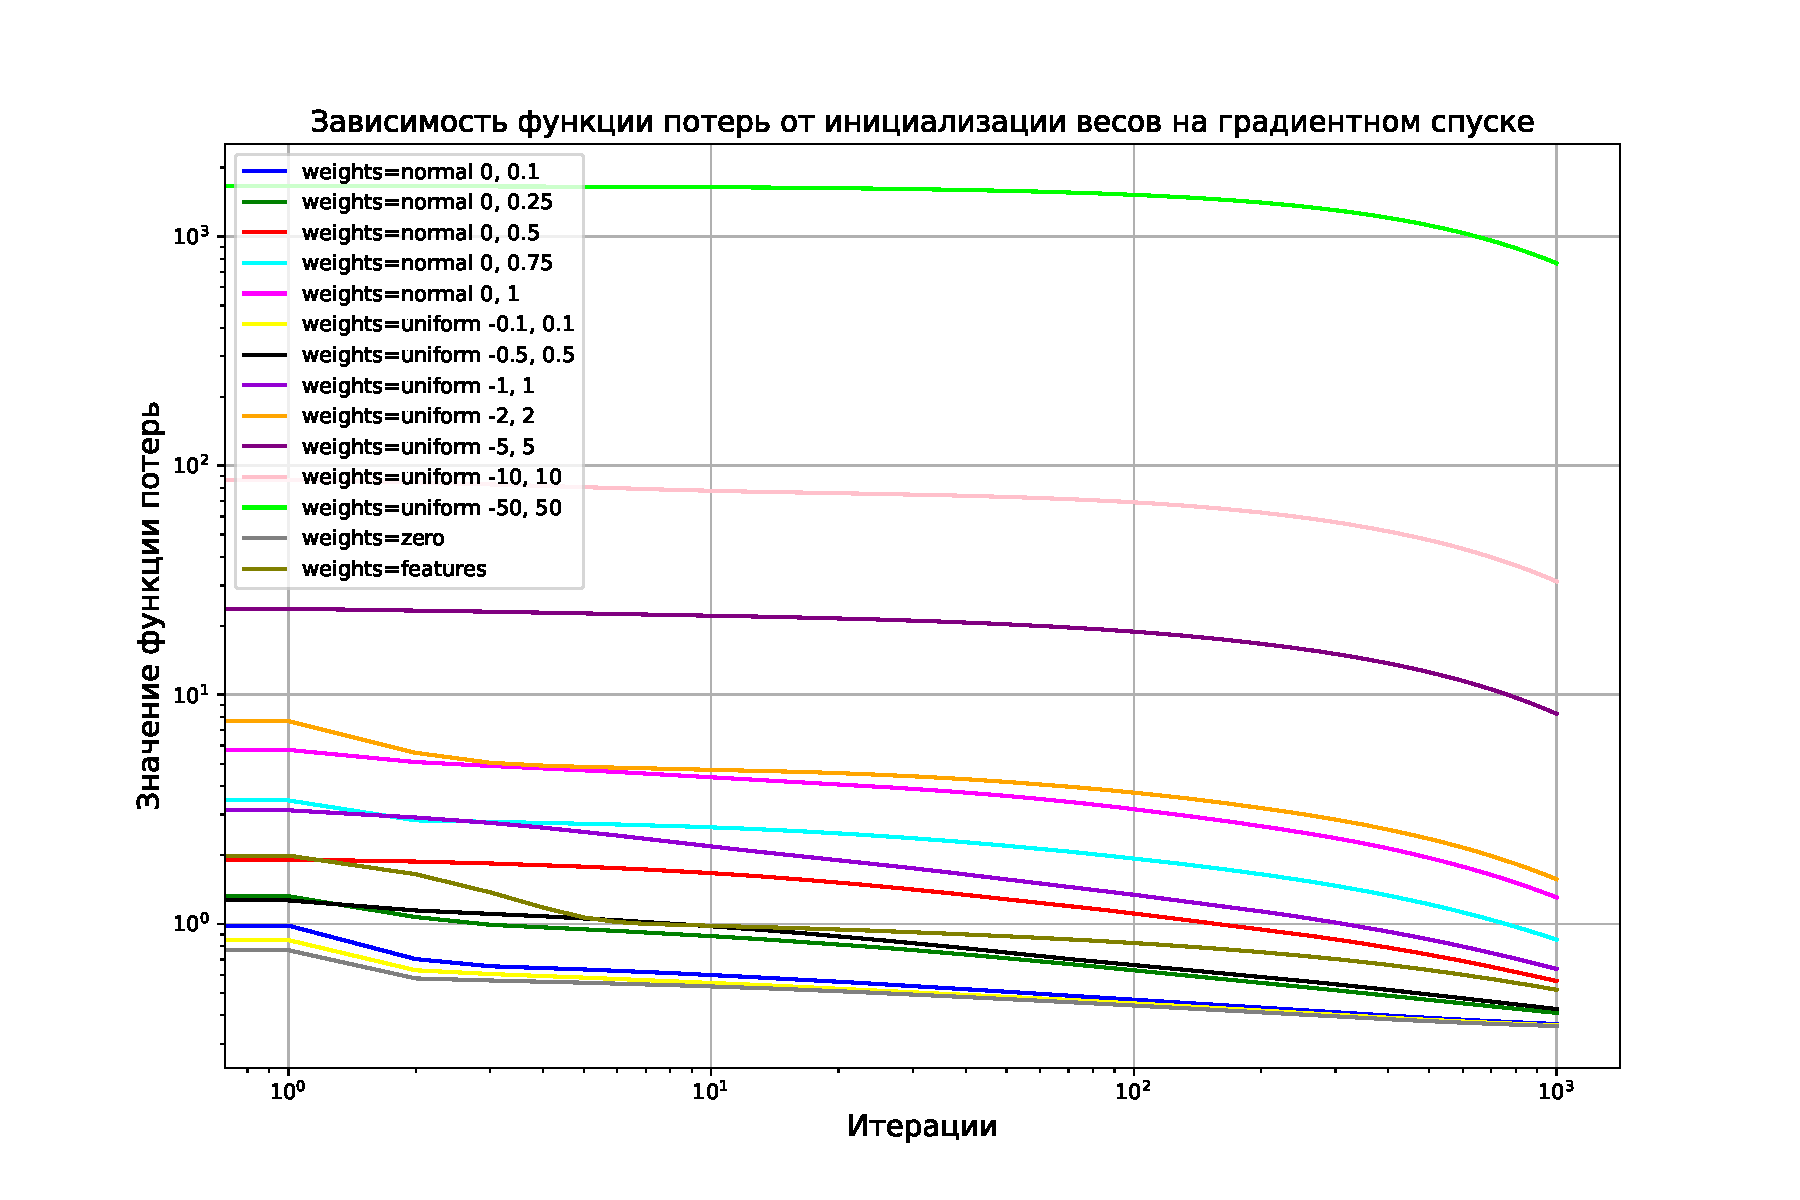
\includegraphics[width=1\linewidth]
    {exp_4_loss_weights.pdf}
    \caption{Значение функции потерь на итерациях модели в зависимости от начального приближения весов}
    \label{fig:exp_4_loss_weights}
\end{figure}

На рисунке \hyperref[fig:exp_4_loss_alpha_1]{12} представлены графики зависимости значения функции потерь на каждой итерации градиентного спуска от начального приближения весов \textit{$ w_0 $}. Как можно заметить из графиков, наилучшая сходимость значений функции потерь модели достигается при \textit{$ w_0 = (0, ... , 0)$}.

\subsubsection{Подбор коэффициента $L_2$-регуляризации}

Будем рассматривать значения \textit{l2\_coef}, равномерно расположенные по логарифмической шкале от $ 10^{-4} $ до $ 10^{4} $.

\begin{figure}[H]
    \centering
    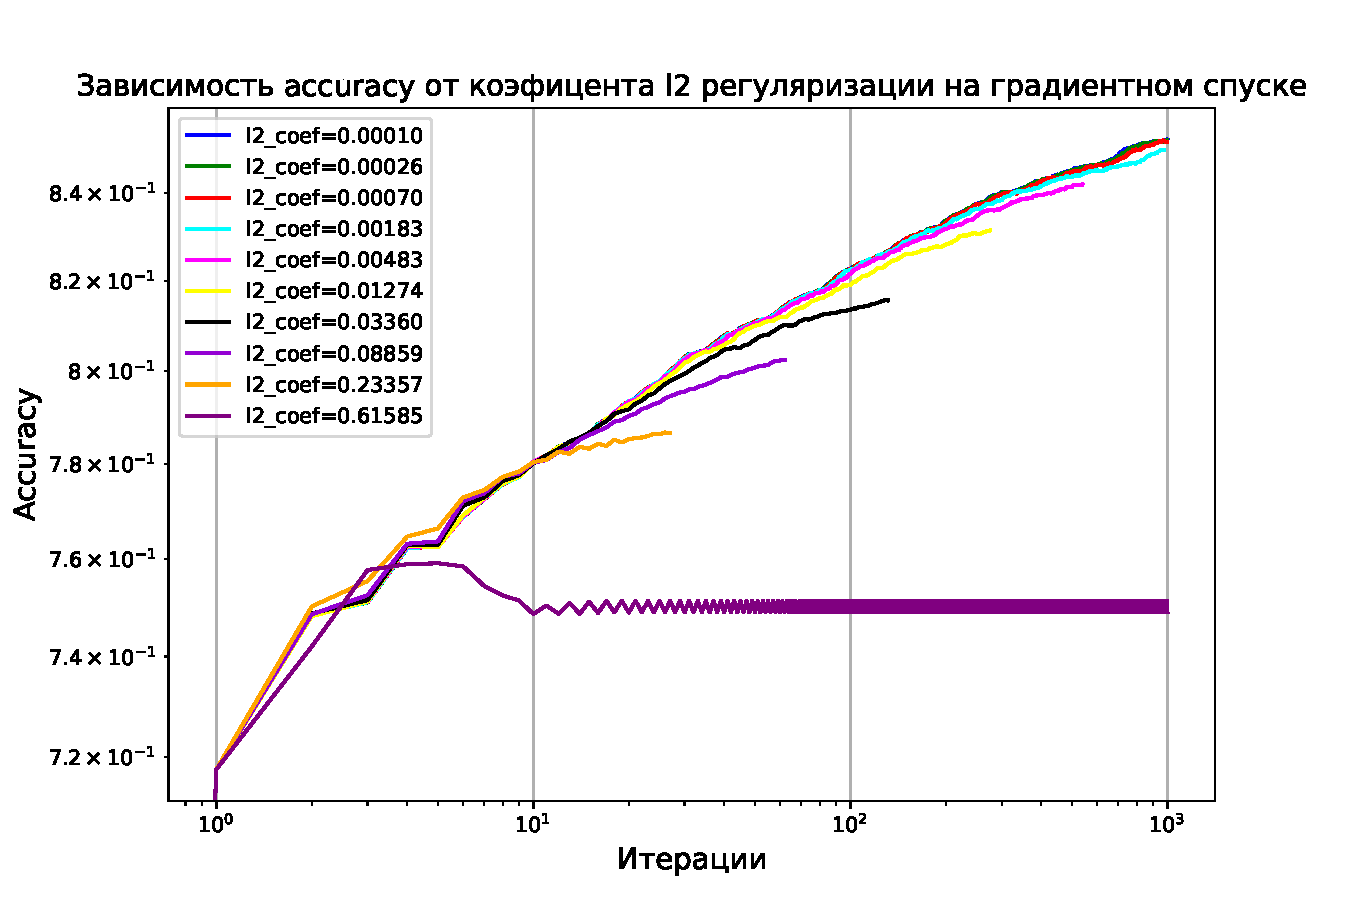
\includegraphics[width=0.7\linewidth]
    {exp_4_acc_l2_1.pdf}
    \caption{Accuracy на итерациях модели в зависимости от параметра \textit{l2\_coef}}
    \label{fig:exp_4_acc_l2_1}
\end{figure}

\begin{figure}[H]
    \centering
    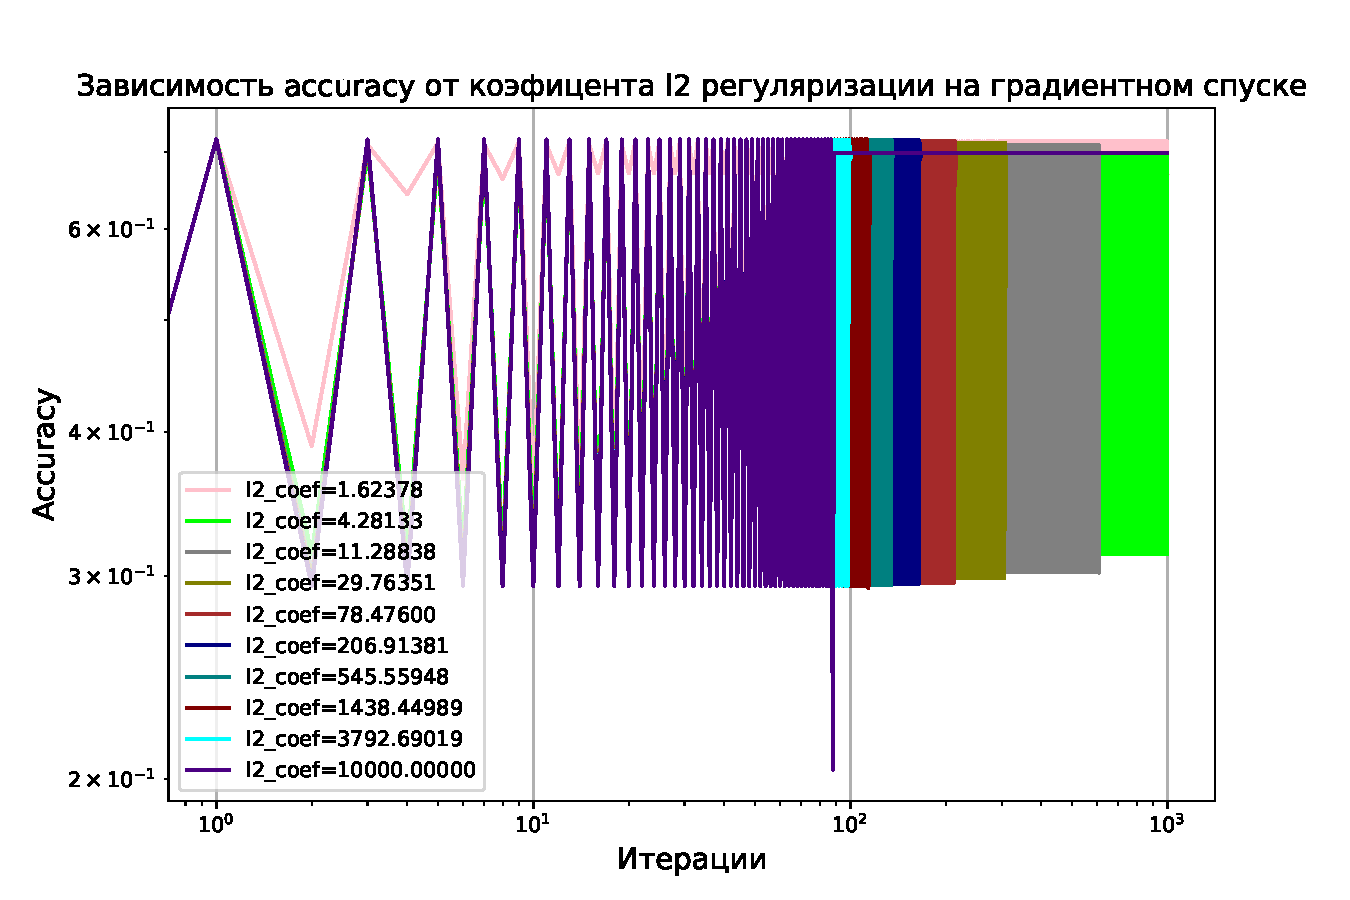
\includegraphics[width=0.7\linewidth]
    {exp_4_acc_l2_2.pdf}
    \caption{Accuracy на итерациях модели в зависимости от параметра \textit{l2\_coef}}
    \label{fig:exp_4_acc_l2_2}
\end{figure}

На рисунках \hyperref[fig:exp_4_acc_l2_1]{13} и \hyperref[fig:exp_4_acc_l2_2]{14} представлены графики зависимости accuracy модели на каждой итерации градиентного спуска от параметра \textit{l2\_coef}. Как можно заметить из графиков, наилучшая точность модели достигается при \textit{l2\_coef = 0.0001}.

\begin{figure}[H]
    \centering
    \includegraphics[width=0.7\linewidth]
    {exp_4_loss_l2_1.pdf}
    \caption{Значение функции потерь на итерациях модели в зависимости от параметра \textit{l2\_coef}}
    \label{fig:exp_4_loss_l2_1}
\end{figure}

\begin{figure}[H]
    \centering
    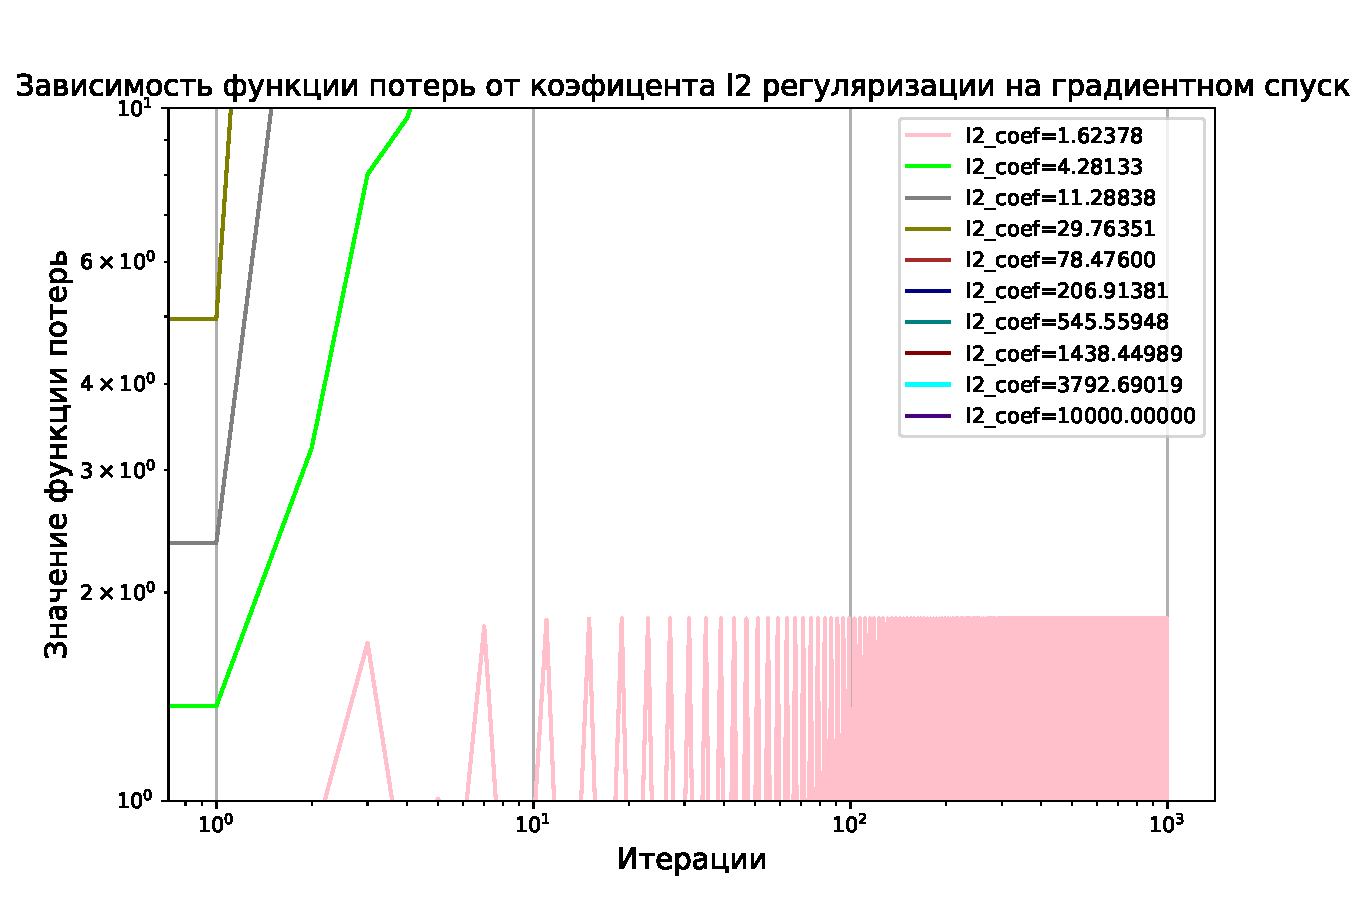
\includegraphics[width=0.7\linewidth]
    {exp_4_loss_l2_2.pdf}
    \caption{Значение функции потерь на итерациях модели в зависимости от параметра \textit{l2\_coef}}
    \label{fig:exp_4_loss_l2_2}
\end{figure}

На рисунках \hyperref[fig:exp_4_loss_l2_1]{15} и \hyperref[fig:exp_4_loss_l2_2]{16} представлены графики зависимости значения функции потерь на каждой итерации градиентного спуска от параметра \textit{l2\_coef}. Как можно заметить из графиков, наилучшая сходимость значений функции потерь модели достигается при \textit{l2\_coef = 0.0001}.

\subsection{Выводы}
Проведенные эксперименты показали следующие лучшие параметры градиентного спуска для задачи логистической регрессии при прочих равных условиях:
\begin{itemize}
    \item \textit{step\_alpha = 0.372759372}
    \item \textit{step\_beta = 0}
    \item \textit{$ w_0 = (0, ... , 0)$}
    \item \textit{l2\_coef = 0.0001}
\end{itemize}


\section{Исследование поведения стохастического градиентного спуска для задачи логистической регрессии в зависимости от \textit{step\_alpha}, \textit{step\_beta} и начального приближения} \label{sec:section6}

\subsection{Постановка задачи}

Исследовать поведение стохастического градиентного спуска для задачи логистической регрессии в зависимости от следующих параметров:
\begin{itemize}
    \item параметр размера шага \texttt{step\_alpha}
    \item параметр размера шага \texttt{step\_beta}
    \item начального приближения
    \item размера подвыборки \textit{batch\_size}
\end{itemize}

Исследование поведения метода подразумевало анализ следующих зависимостей:
\begin{itemize}
    \item зависимость значения функции потерь от эпохи метода
    \item зависимость точности (accuracy) эпохи метода
\end{itemize}

\subsection{Реализация}

Во всех экспериментах до подбора наилучшего параметра при прочих равных увсловиях брались как тестирующие значения параметры:
\begin{itemize}
    \item \textit{step\_beta = 0}
    \item \textit{batch\_size = 500}
    \item \textit{l2\_coef = 0.001}
    \item \textit{max\_iter = 1000}
\end{itemize}

После нахождения наилучшего параметра - использовался он.

\subsubsection{Подбор параметра \textit{step\_alpha}}

Будем рассматривать значения \textit{step\_alpha}, равномерно расположенные по логарифмической шкале от $ 10^{-4} $ до 10.

\begin{figure}[H]
    \centering
    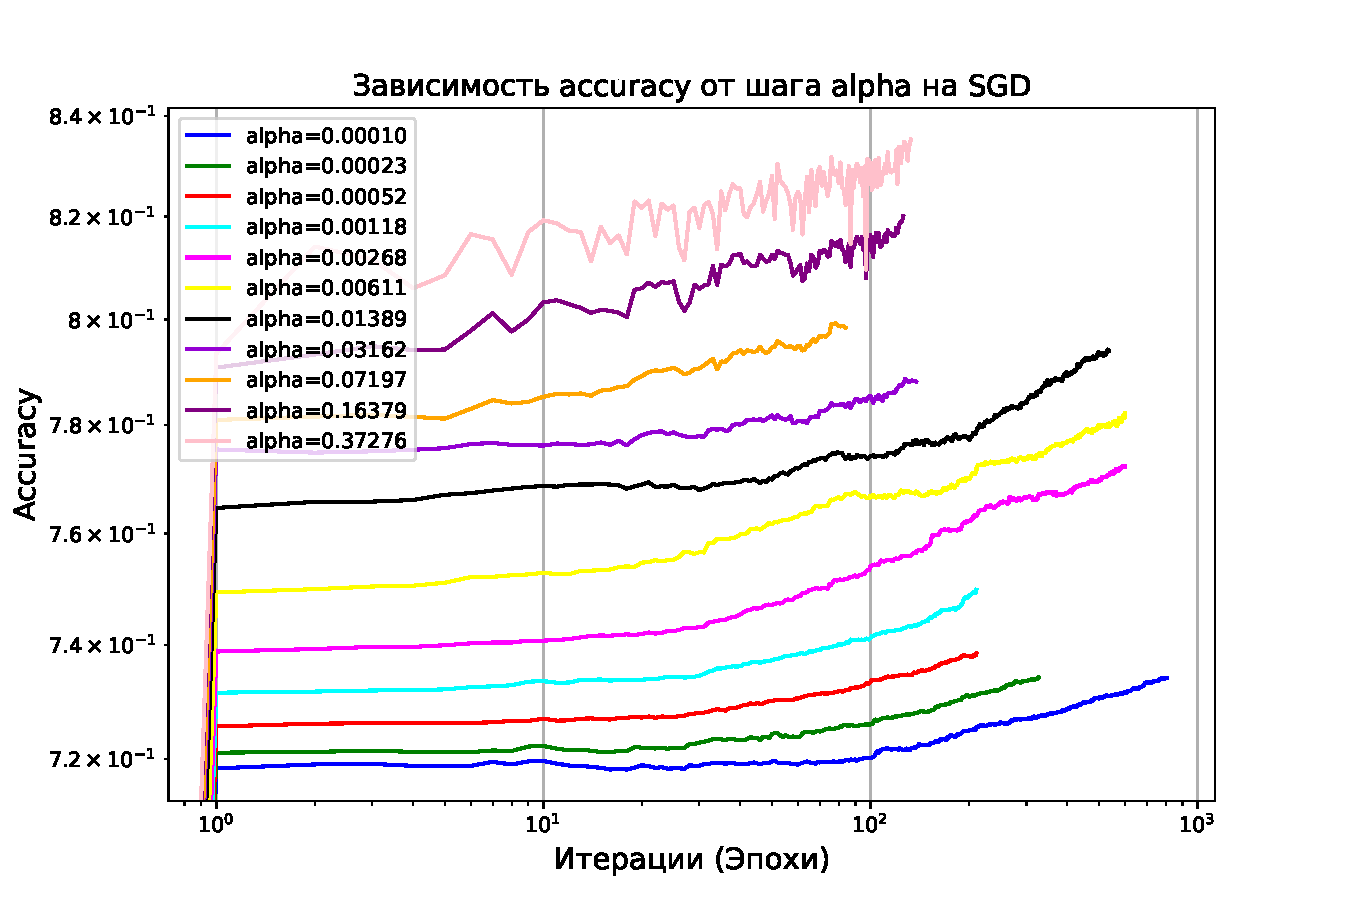
\includegraphics[width=0.7\linewidth]
    {exp_5_acc_alpha_1.pdf}
    \caption{Accuracy на эпохах модели в зависимости от параметра \textit{step\_alpha}}
    \label{fig:exp_5_acc_alpha_1}
\end{figure}

\begin{figure}[H]
    \centering
    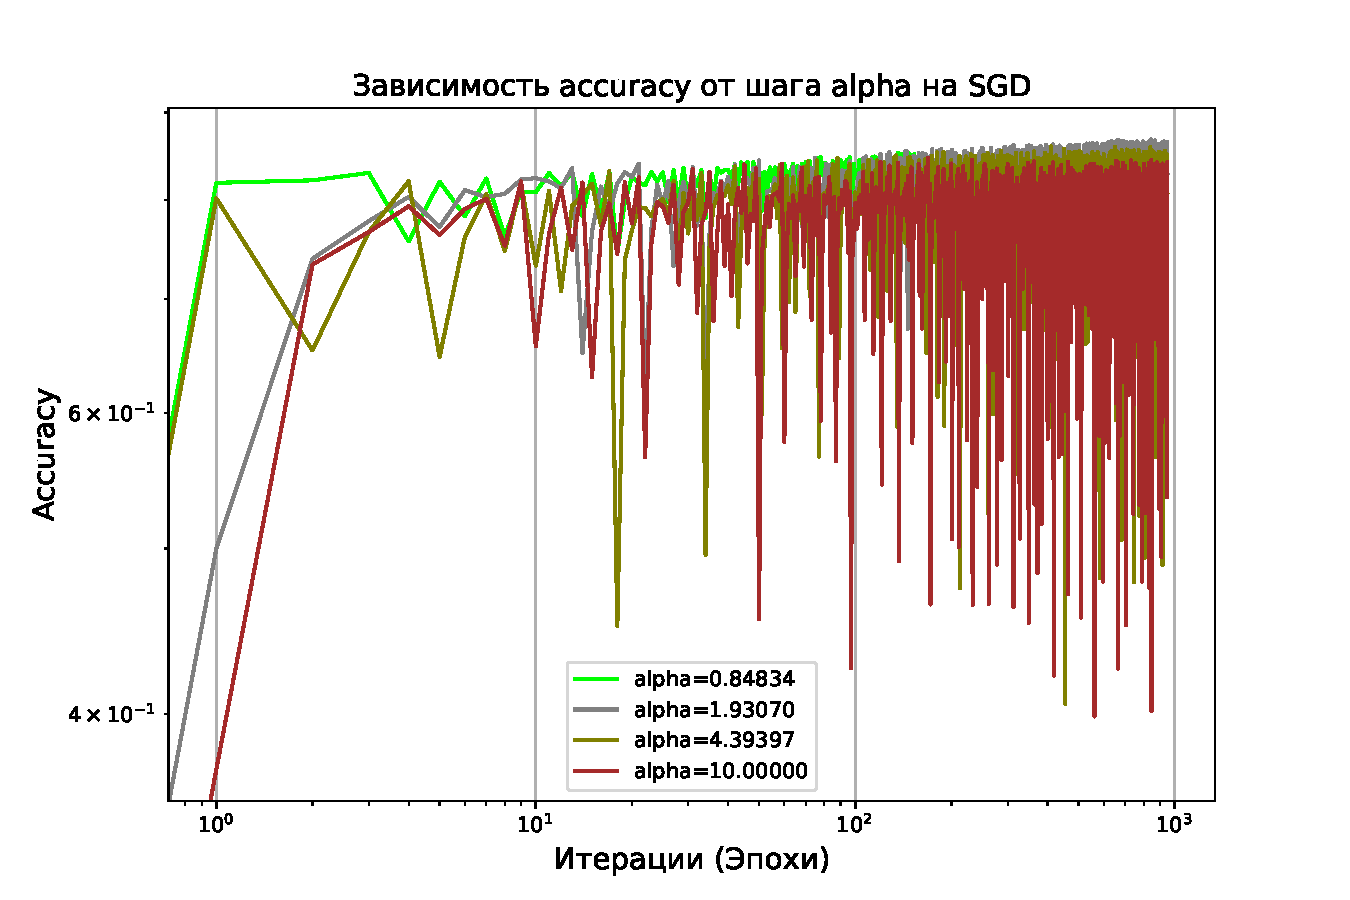
\includegraphics[width=0.7\linewidth]
    {exp_5_acc_alpha_2.pdf}
    \caption{Accuracy на эпохах модели в зависимости от параметра \textit{step\_alpha}}
    \label{fig:exp_5_acc_alpha_2}
\end{figure}

На рисунках \hyperref[fig:exp_5_acc_alpha_1]{17} и \hyperref[fig:exp_5_acc_alpha_2]{18} представлены графики зависимости accuracy модели на каждой эпохе стохастического градиентного спуска от параметра \textit{step\_alpha}. Как можно заметить из графиков, наилучшая точность модели достигается при \textit{step\_alpha = 0.372759372}.

\begin{figure}[H]
    \centering
    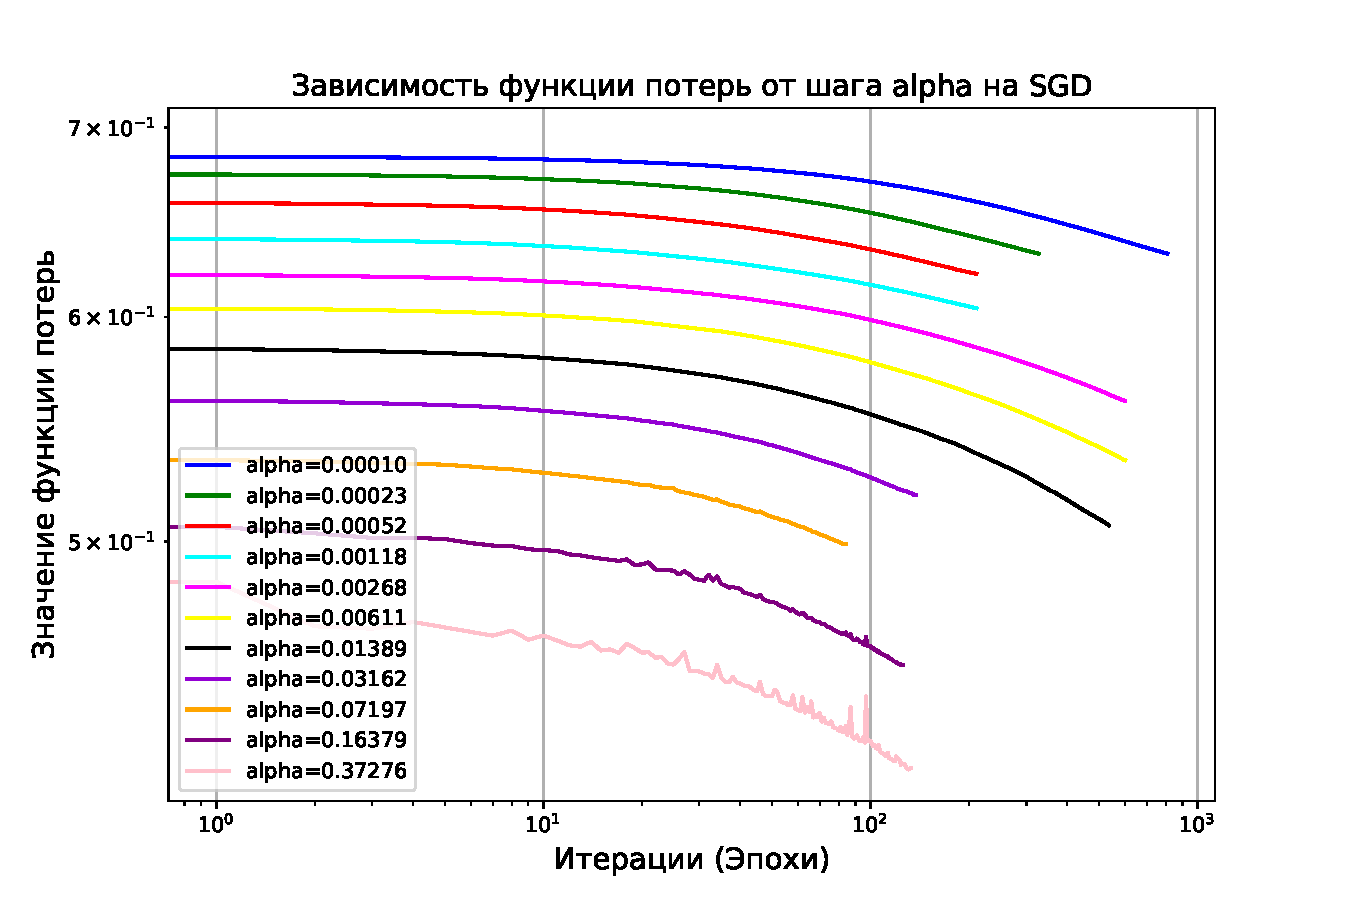
\includegraphics[width=0.7\linewidth]
    {exp_5_loss_alpha_1.pdf}
    \caption{Значение функции потерь на эпохах модели в зависимости от параметра \textit{step\_alpha}}
    \label{fig:exp_5_loss_alpha_1}
\end{figure}

\begin{figure}[H]
    \centering
    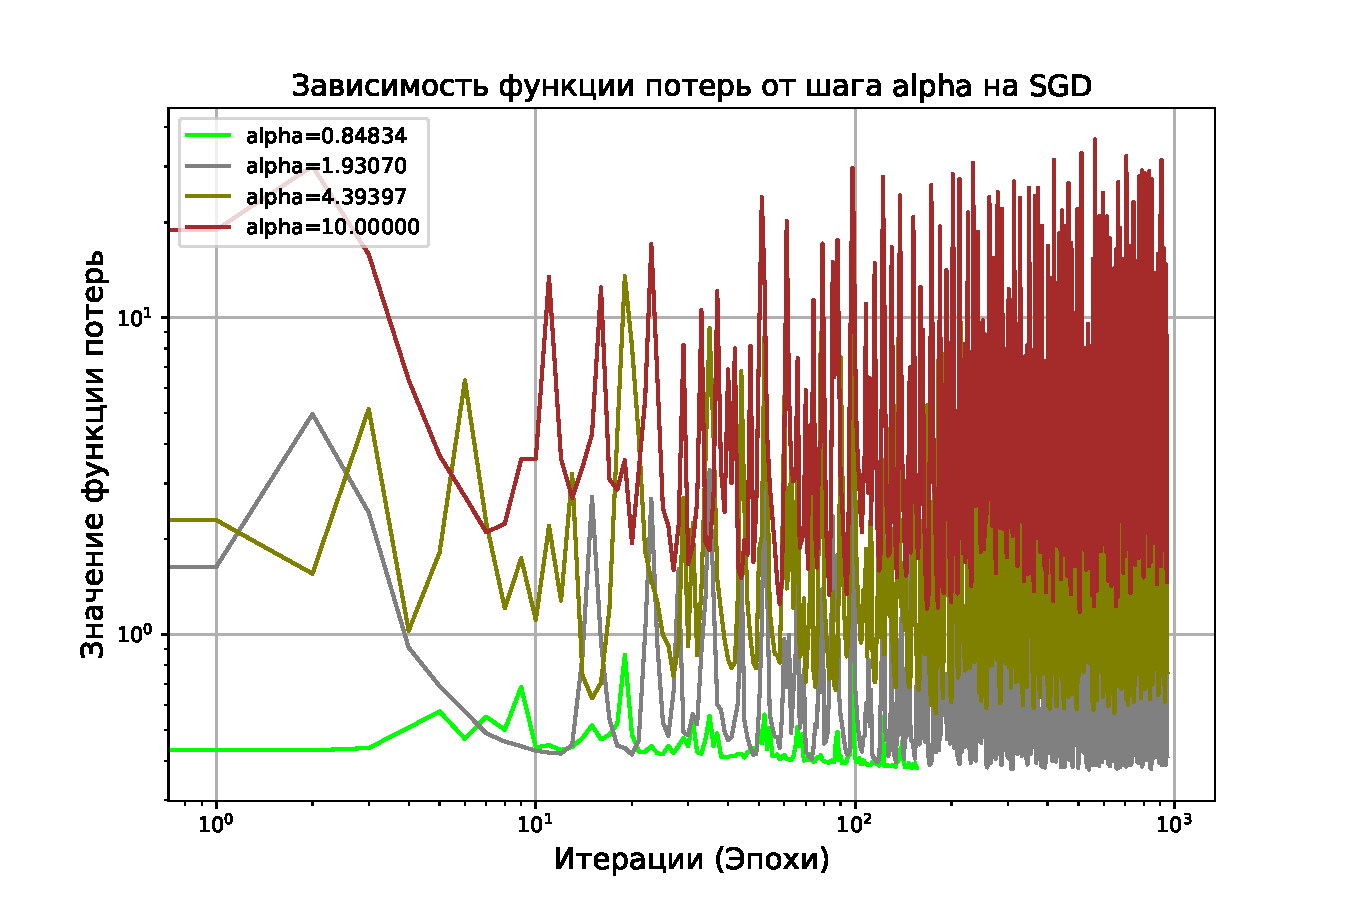
\includegraphics[width=0.7\linewidth]
    {exp_5_loss_alpha_2.pdf}
    \caption{Значение функции потерь на эпохах модели в зависимости от параметра \textit{step\_alpha}}
    \label{fig:exp_5_loss_alpha_2}
\end{figure}

На рисунках \hyperref[fig:exp_5_loss_alpha_1]{19} и \hyperref[fig:exp_5_loss_alpha_2]{20} представлены графики зависимости значения функции потерь на каждой эпохе стохастического градиентного спуска от параметра \textit{step\_alpha}. Как можно заметить из графиков, наилучшая сходимость значений функции потерь модели достигается при \textit{step\_alpha = 0.372759372}.

\subsubsection{Подбор параметра \textit{step\_beta}}

Будем рассматривать значения \textit{step\_beta} среди следующего множества значений: \( \{0, \ 0.0001, \ 0.001, \ 0.005, \ 0.01, \ 0.05, \ 0.1, \ 0.2, \ 0.3, \ 0.5, \ 0.7, \ 1, \ 2, \ 3, \ 4, \ 5, \ 10, \ 15, \\ 25, \ 50, \ 75, \ 100\} \).

\begin{figure}[H]
    \centering
    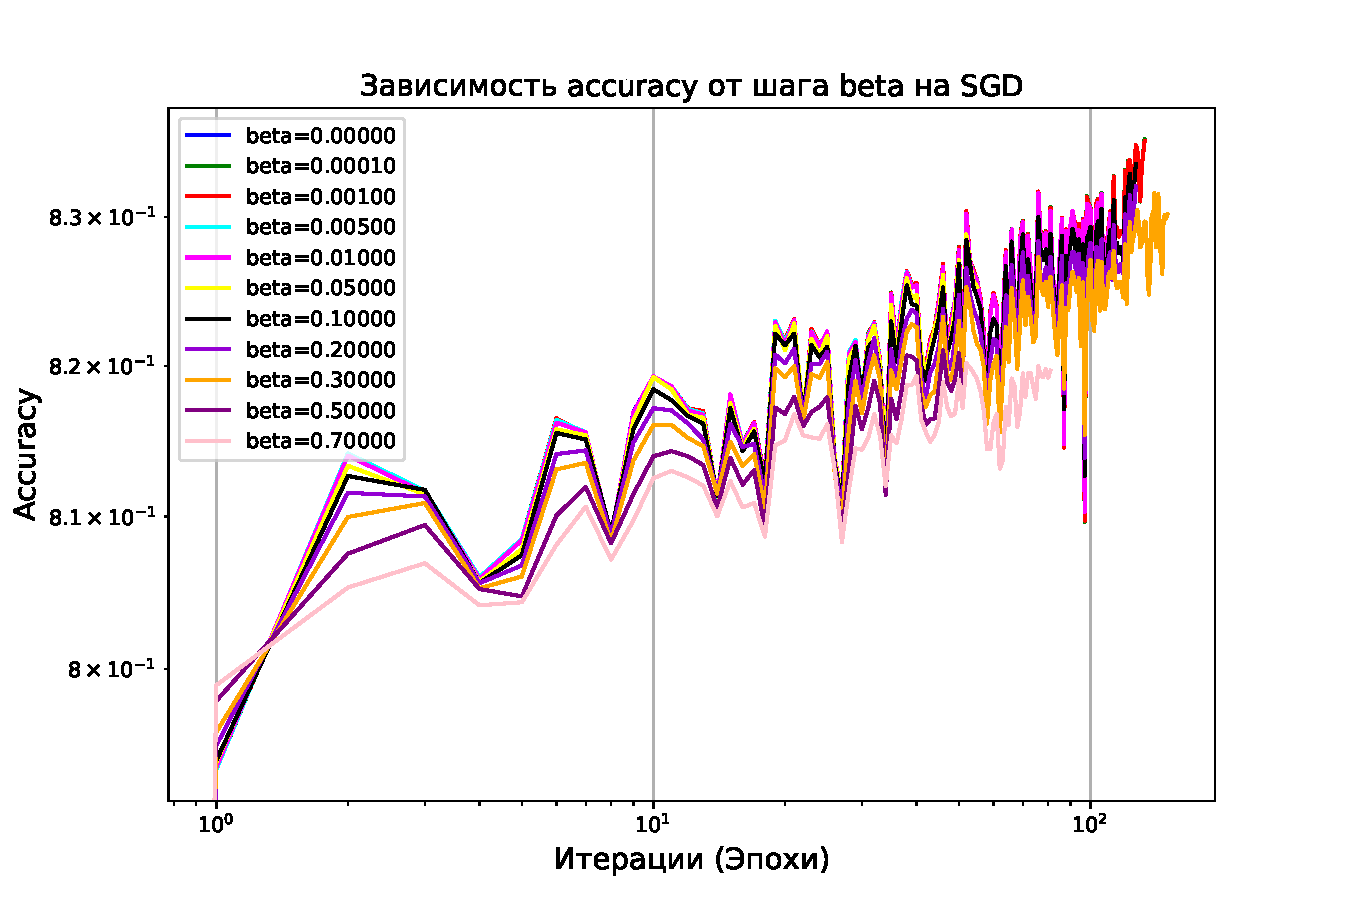
\includegraphics[width=0.7\linewidth]
    {exp_5_acc_beta_1.pdf}
    \caption{Accuracy на эпохах модели в зависимости от параметра \textit{step\_beta}}
    \label{fig:exp_5_acc_beta_1}
\end{figure}

\begin{figure}[H]
    \centering
    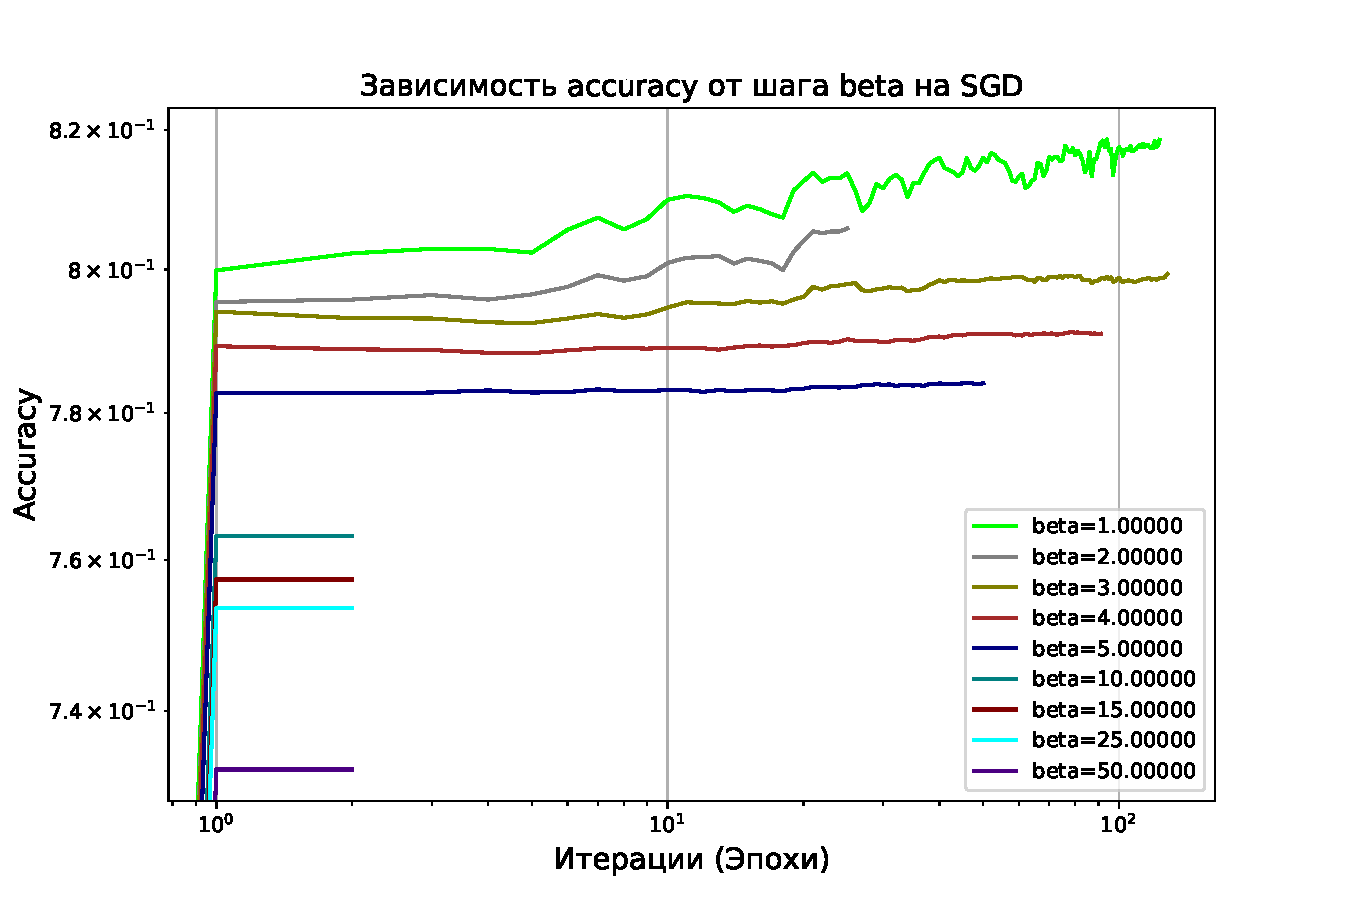
\includegraphics[width=0.7\linewidth]
    {exp_5_acc_beta_2.pdf}
    \caption{Accuracy на эпохах модели в зависимости от параметра \textit{step\_beta}}
    \label{fig:exp_5_acc_beta_2}
\end{figure}

На рисунках \hyperref[fig:exp_5_acc_beta_1]{21} и \hyperref[fig:exp_5_acc_beta_2]{22} представлены графики зависимости accuracy модели на каждой эпохе стохастического градиентного спуска от параметра \textit{step\_beta}. Как можно заметить из графиков, наилучшая точность модели достигается при \textit{step\_beta = 0.001}.

\begin{figure}[H]
    \centering
    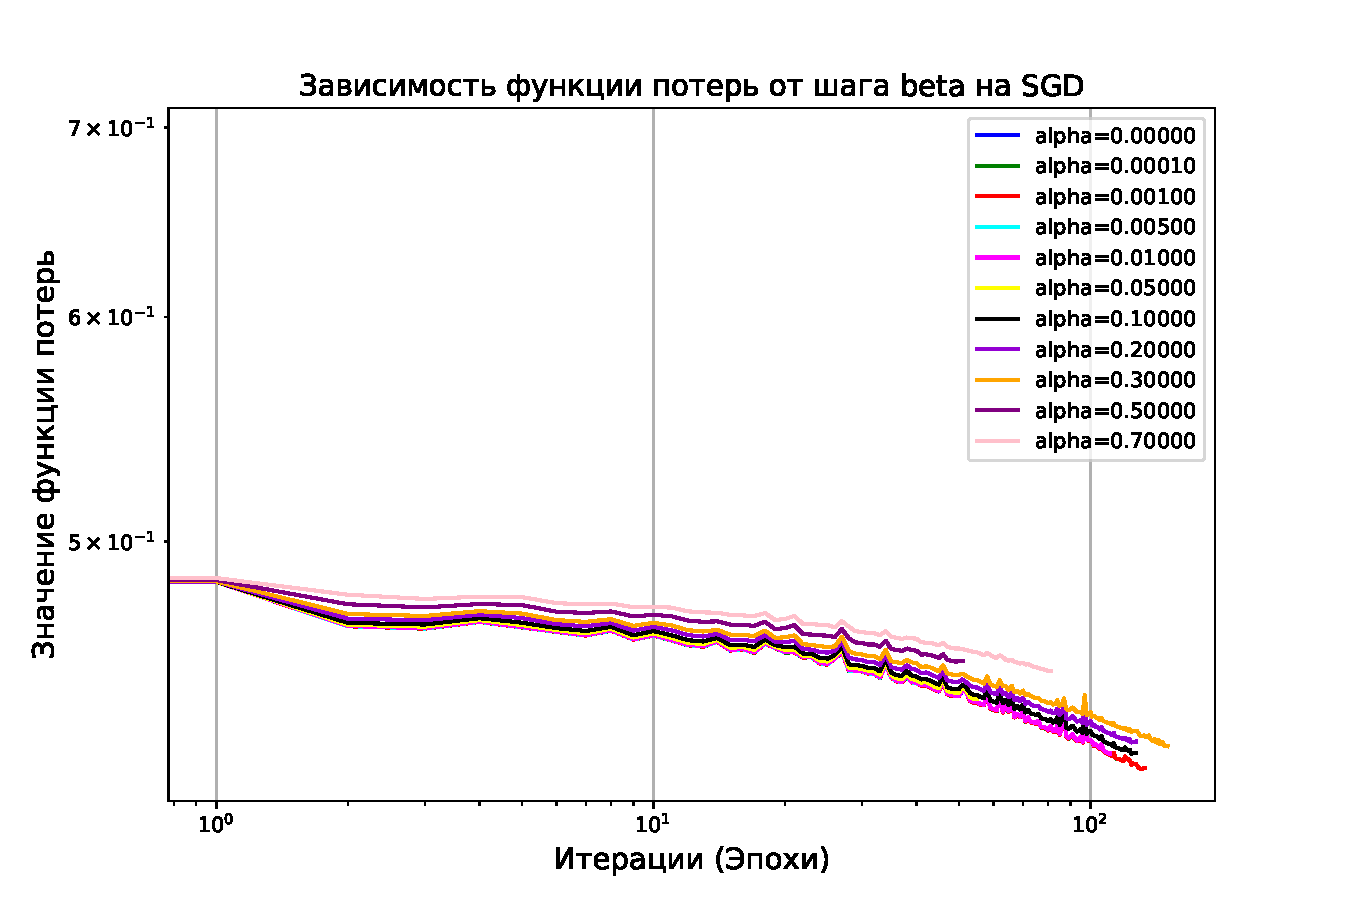
\includegraphics[width=0.7\linewidth]
    {exp_5_loss_beta_1.pdf}
    \caption{Значение функции потерь на эпохах модели в зависимости от параметра \textit{step\_beta}}
    \label{fig:exp_5_loss_beta_1}
\end{figure}

\begin{figure}[H]
    \centering
    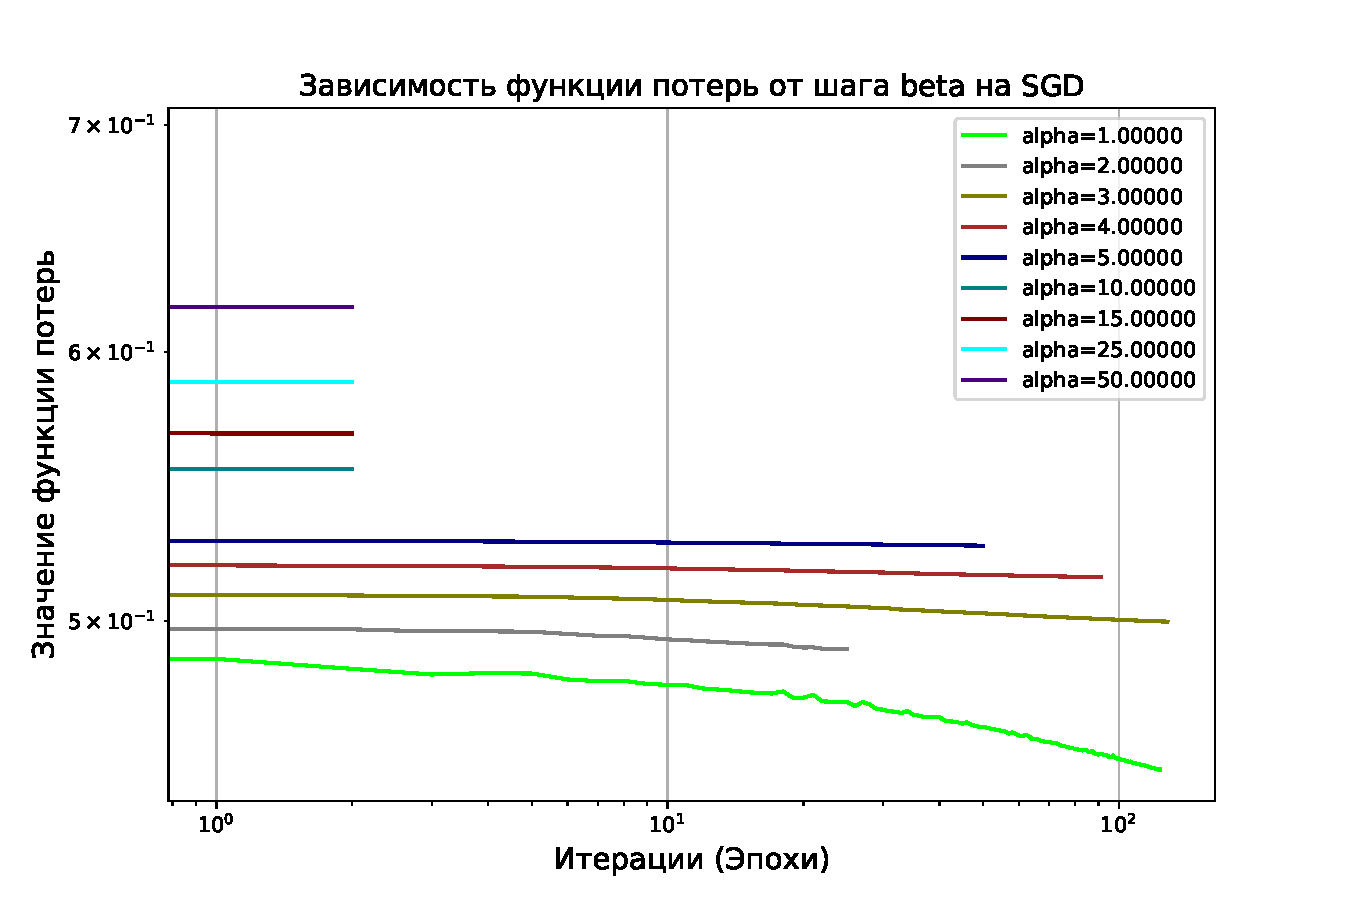
\includegraphics[width=0.7\linewidth]
    {exp_5_loss_beta_2.pdf}
    \caption{Значение функции потерь на эпохах модели в зависимости от параметра \textit{step\_beta}}
    \label{fig:exp_5_loss_beta_2}
\end{figure}

На рисунках \hyperref[fig:exp_5_loss_beta_1]{23} и \hyperref[fig:exp_5_loss_beta_2]{24} представлены графики зависимости значения функции потерь на каждой  эпохе стохастического градиентного спуска от параметра \textit{step\_beta}. Как можно заметить из графиков, наилучшая сходимость значений функции потерь модели достигается при \textit{step\_beta = 0.001}.

\subsubsection{Подбор начального приближения весов \textit{$ w_0 $}}

Будем рассматривать значения начального приближения весов \textit{$ w_0 $}, используя функции \textit{Numpy}, такие как \textit{np.random.normal} и \textit{np.random.uniform}, соответствующие нормальному и равномерному распределениям. Рассмотрим значения начального приближения весов, соответствующие данным распределениям со следующими параметрами:
\begin{itemize}
    \item normal 0, 0.1
    \item normal 0, 0.25
    \item normal 0, 0.5
    \item normal 0, 0.75
    \item normal 0, 1
    \item uniform -0.1, 0.1
    \item uniform -0.5, 0.5
    \item uniform -1, 1
    \item uniform -2, 2
    \item uniform -5, 5
    \item uniform -10, 10
    \item uniform -50, 50
\end{itemize}

А также начальное приближение весов: нулями и по формуле: $ w_j = \frac{\langle f_j, y
\rangle}{\langle f_j, f_j \rangle}, \\ \text{где } y \text{ — вектор меток, } f_j
\text{ — столбец признака, а }  w_j \text{ - } j \text{-й элемент вектора весов } w_0$

\begin{figure}[H]
    \centering
    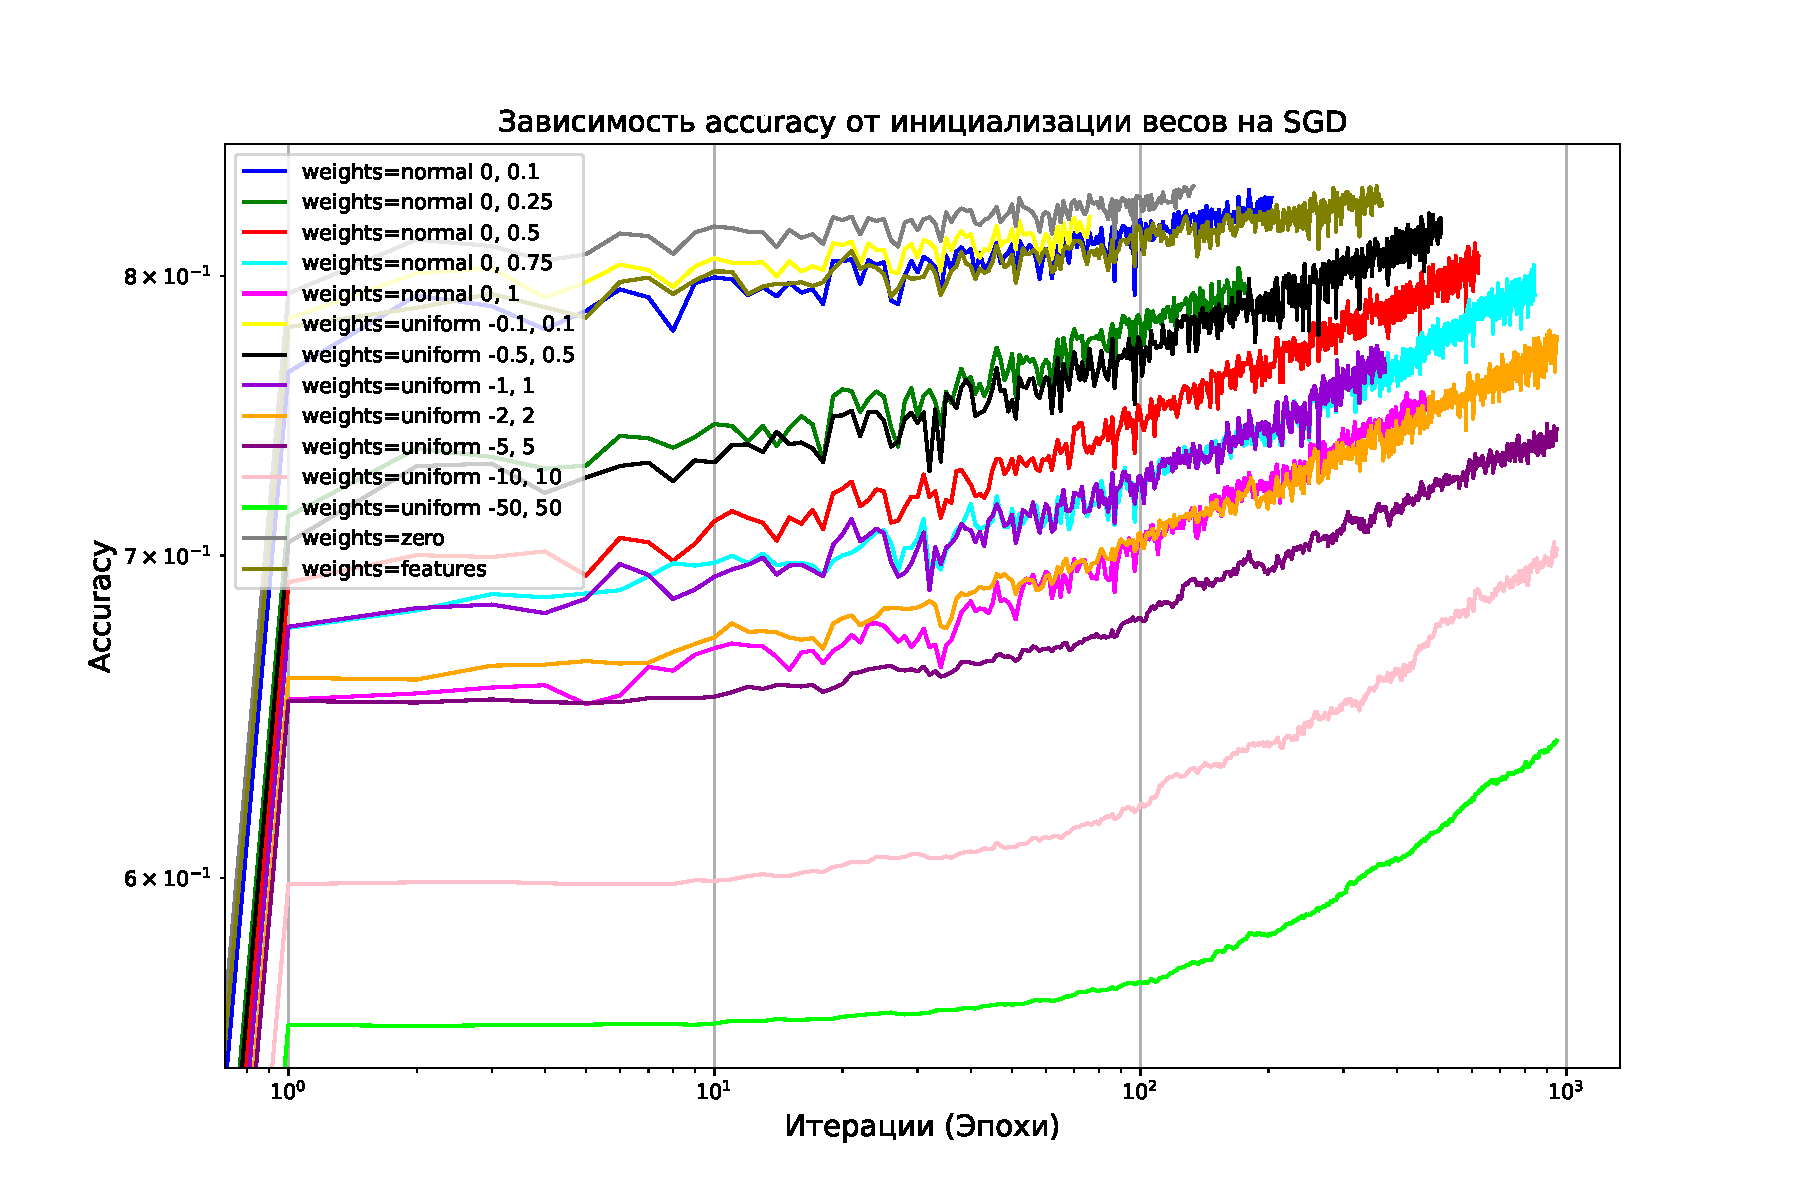
\includegraphics[width=1\linewidth]
    {exp_5_acc_weights.pdf}
    \caption{Accuracy на эпохах модели в зависимости от начального приближения весов}
    \label{fig:exp_5_acc_weights}
\end{figure}

На рисунке \hyperref[fig:exp_5_acc_alpha_1]{25} представлены графики зависимости accuracy модели на каждой эпохе стохастического градиентного спуска от начального приближения весов \textit{$ w_0 $}. Как можно заметить из графиков, наилучшая точность модели достигается при \textit{$ w_0 = (0, ... , 0)$}.

\begin{figure}[H]
    \centering
    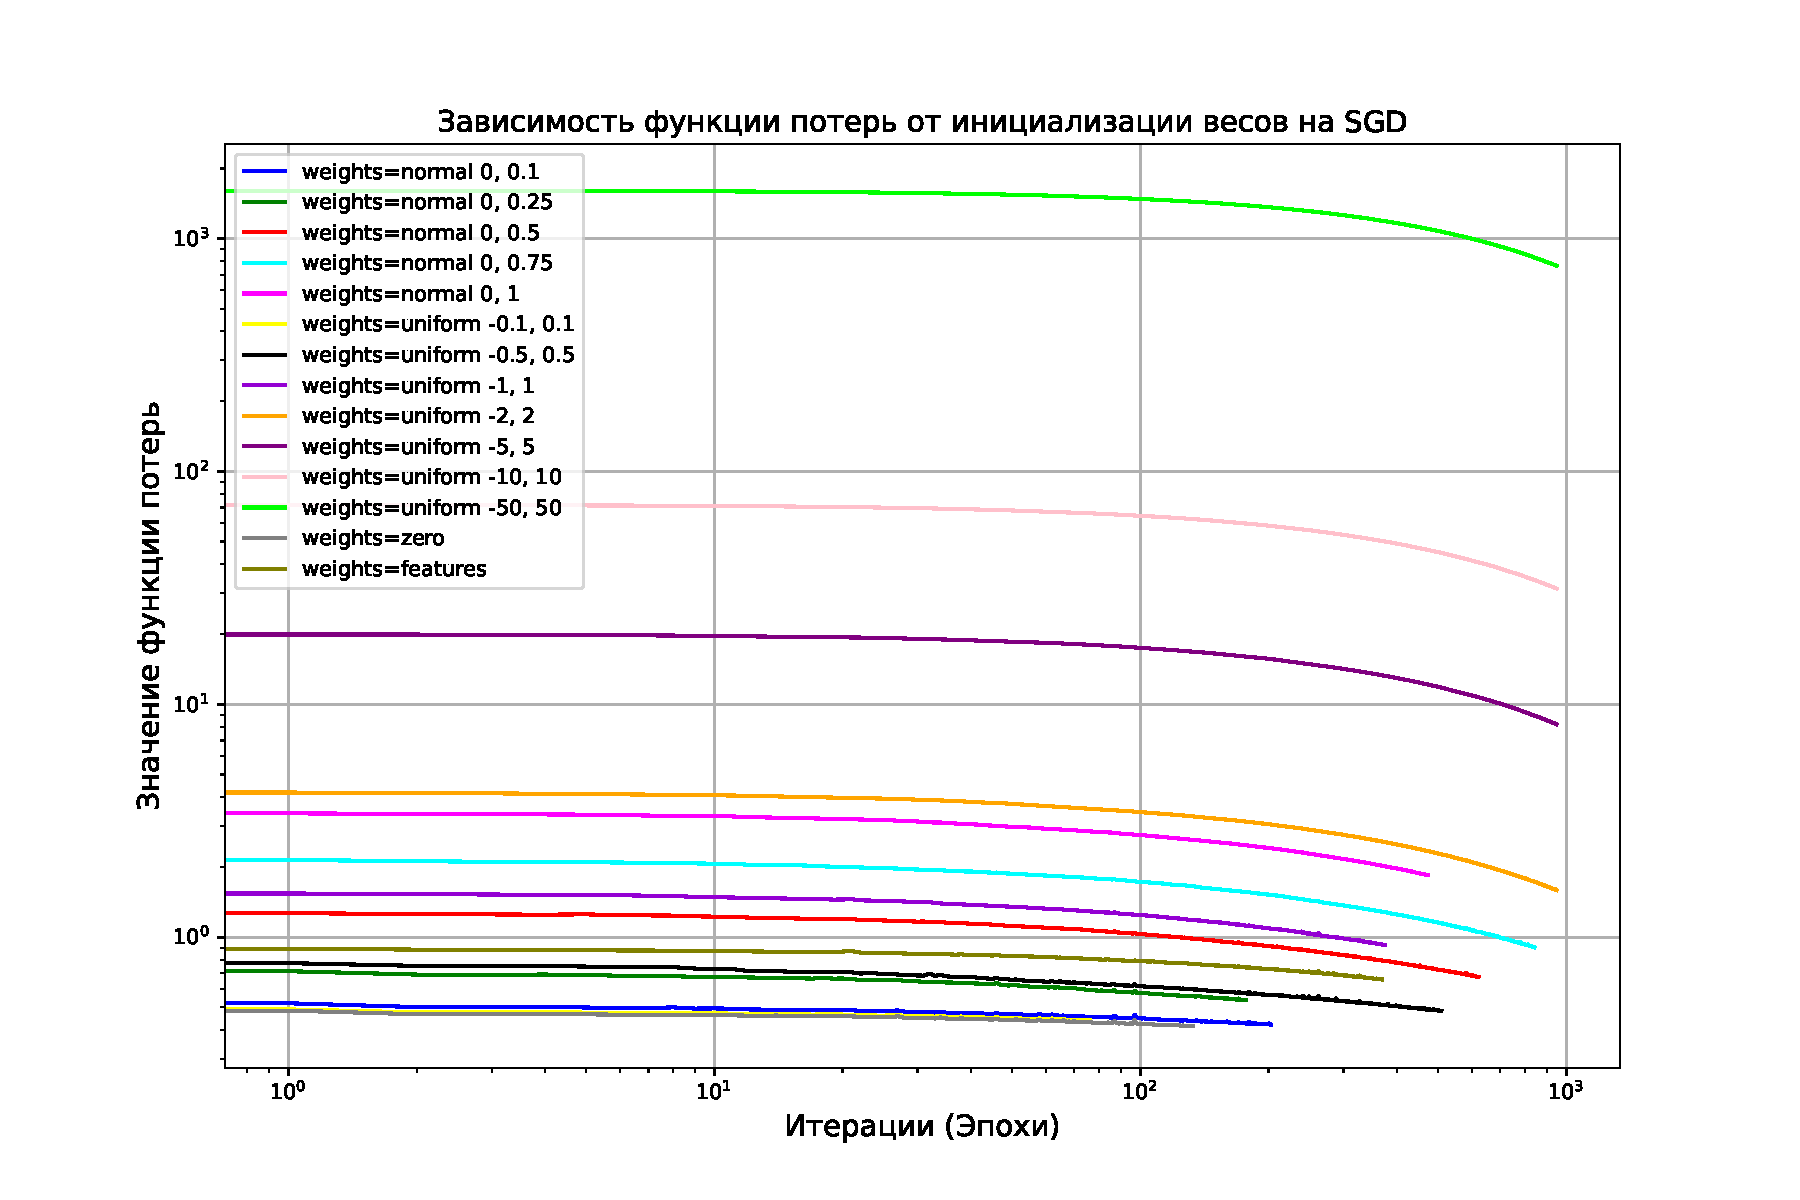
\includegraphics[width=1\linewidth]
    {exp_5_loss_weights.pdf}
    \caption{Значение функции потерь на эпохах модели в зависимости от начального приближения весов}
    \label{fig:exp_5_loss_weights}
\end{figure}

На рисунке \hyperref[fig:exp_5_loss_alpha_1]{26} представлены графики зависимости значения функции потерь на каждой эпохе стохастического градиентного спуска от начального приближения весов \textit{$ w_0 $}. Как можно заметить из графиков, наилучшая сходимость значений функции потерь модели достигается при \textit{$ w_0 = (0, ... , 0)$}.

\subsubsection{Подбор размера подвыборки \textit{batch\_size}}

Будем рассматривать значения \textit{batch\_size} среди следующего множества значений: \( \{100, \ 200, \ 300, \ 400, \ 500, \ 750, \ 1000, \ 1500, \ 2000, \ 5000, \ 10000, \ 20000\} \).

\begin{figure}[H]
    \centering
    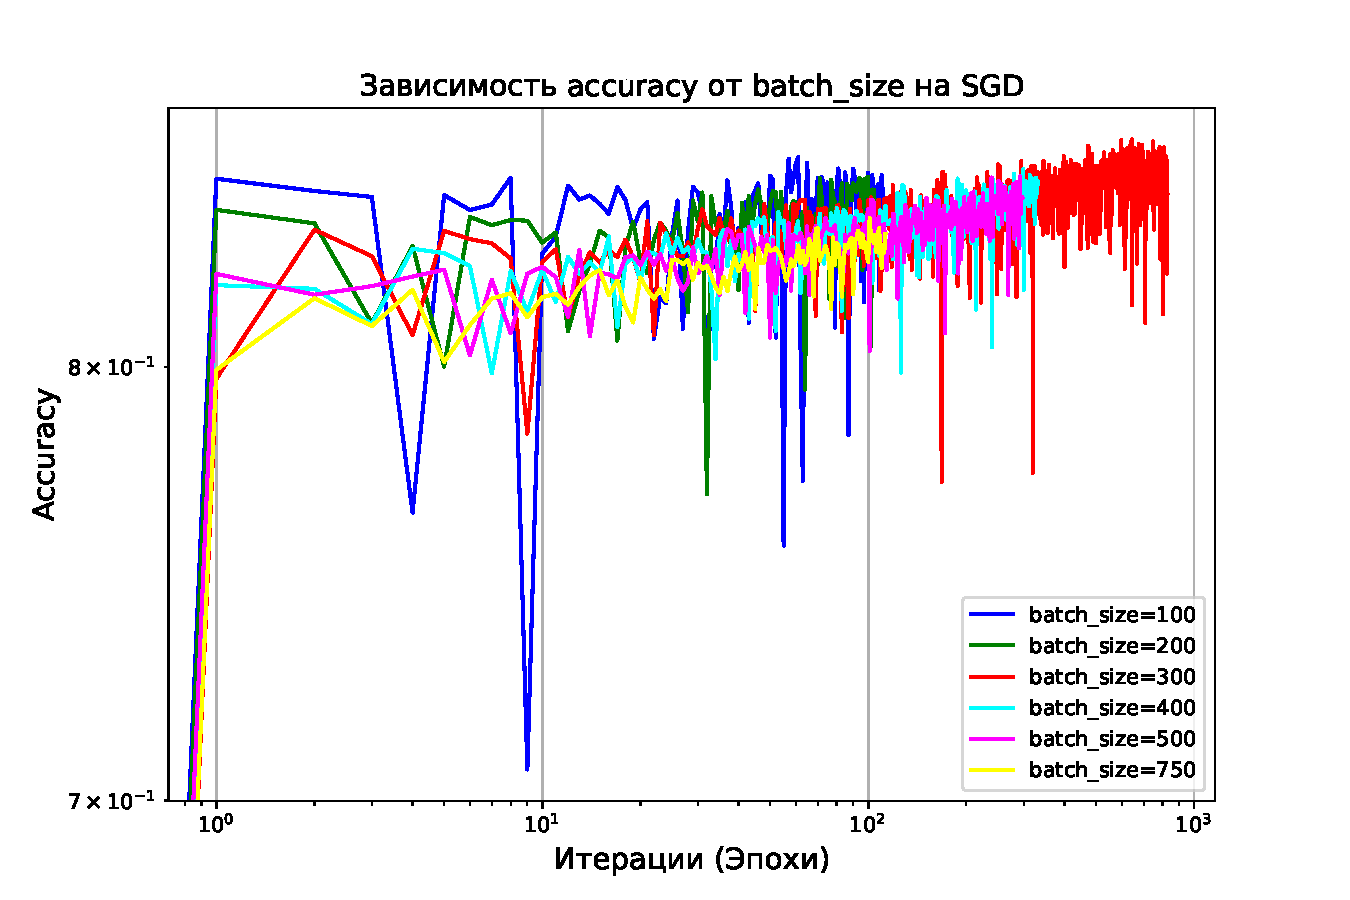
\includegraphics[width=0.7\linewidth]
    {exp_5_acc_batches_1.pdf}
    \caption{Accuracy на эпохах модели в зависимости от параметра \textit{batch\_size}}
    \label{fig:exp_5_acc_batches_1}
\end{figure}

\begin{figure}[H]
    \centering
    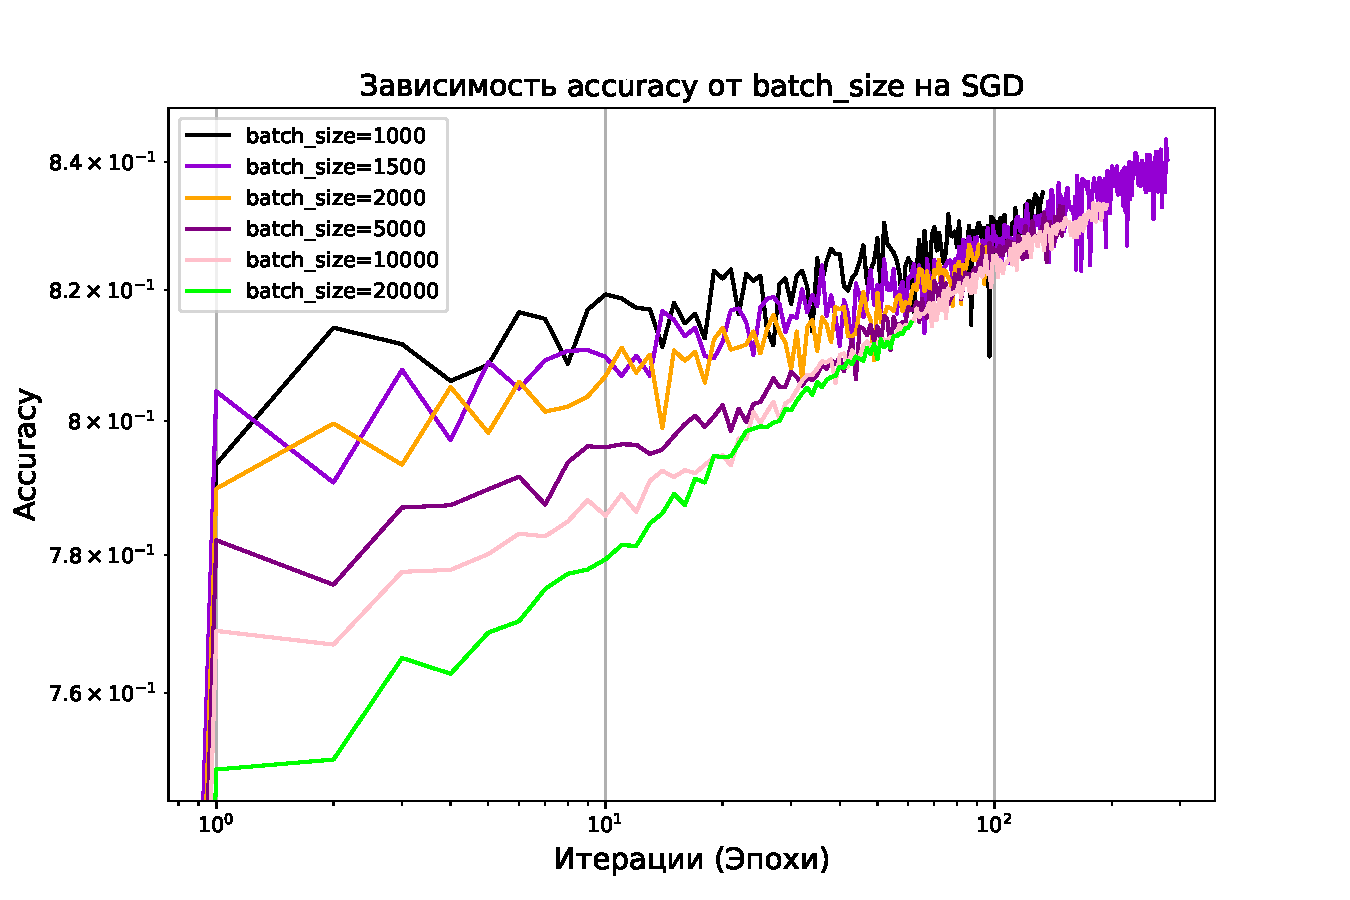
\includegraphics[width=0.7\linewidth]
    {exp_5_acc_batches_2.pdf}
    \caption{Accuracy на эпохах модели в зависимости от параметра \textit{batch\_size}}
    \label{fig:exp_5_acc_batches_2}
\end{figure}

На рисунках \hyperref[fig:exp_5_acc_batches_1]{27} и \hyperref[fig:exp_5_acc_batches_2]{28} представлены графики зависимости accuracy модели на каждой эпохе стохастического градиентного спуска от параметра \textit{batch\_size}. Как можно заметить из графиков, наилучшая точность модели достигается при \textit{batch\_size = 300}.

\begin{figure}[H]
    \centering
    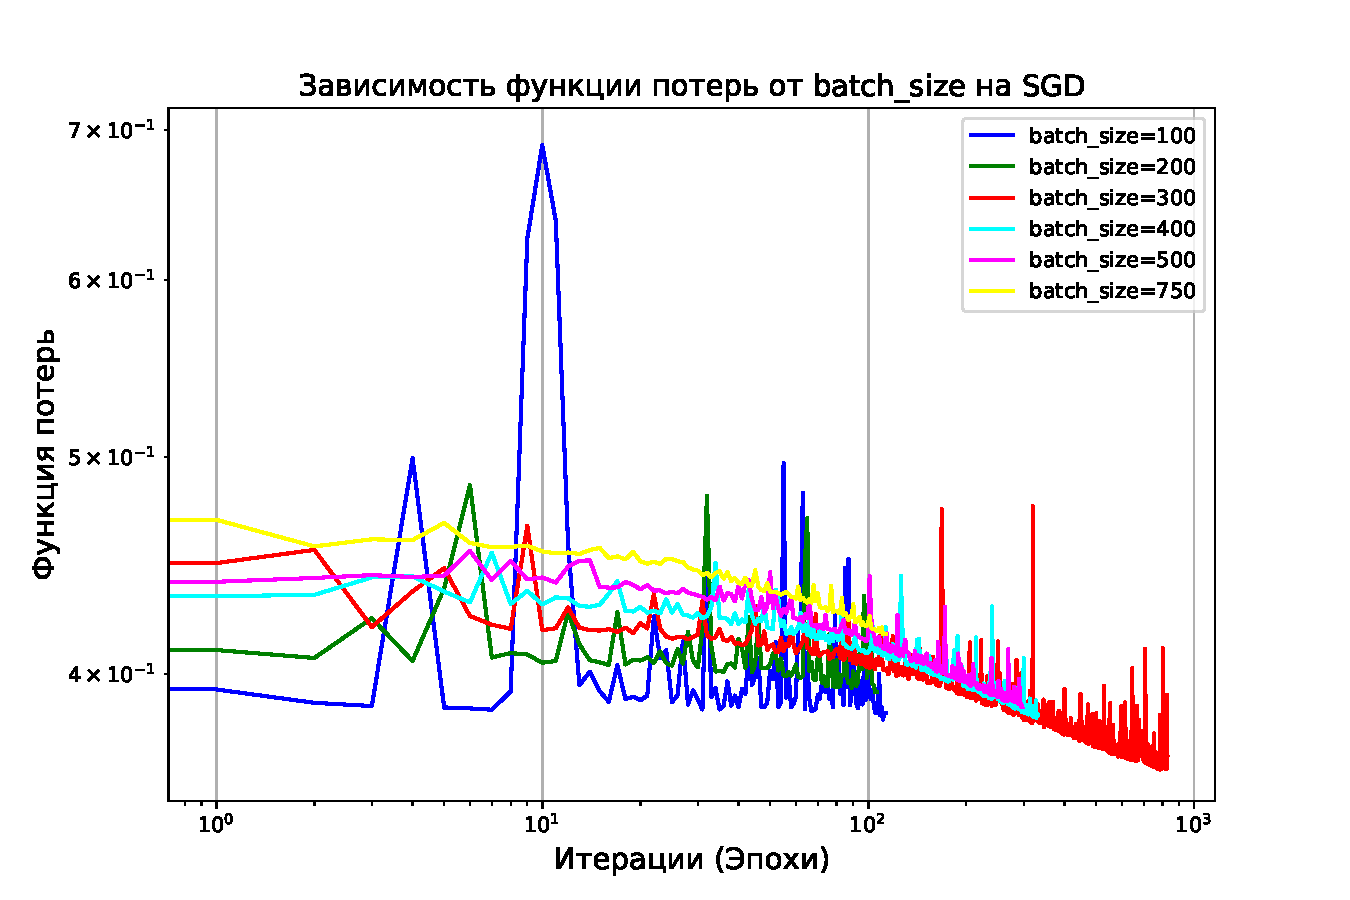
\includegraphics[width=0.7\linewidth]
    {exp_5_loss_batches_1.pdf}
    \caption{Значение функции потерь на эпохах модели в зависимости от параметра \textit{batch\_size}}
    \label{fig:exp_5_loss_batches_1}
\end{figure}

\begin{figure}[H]
    \centering
    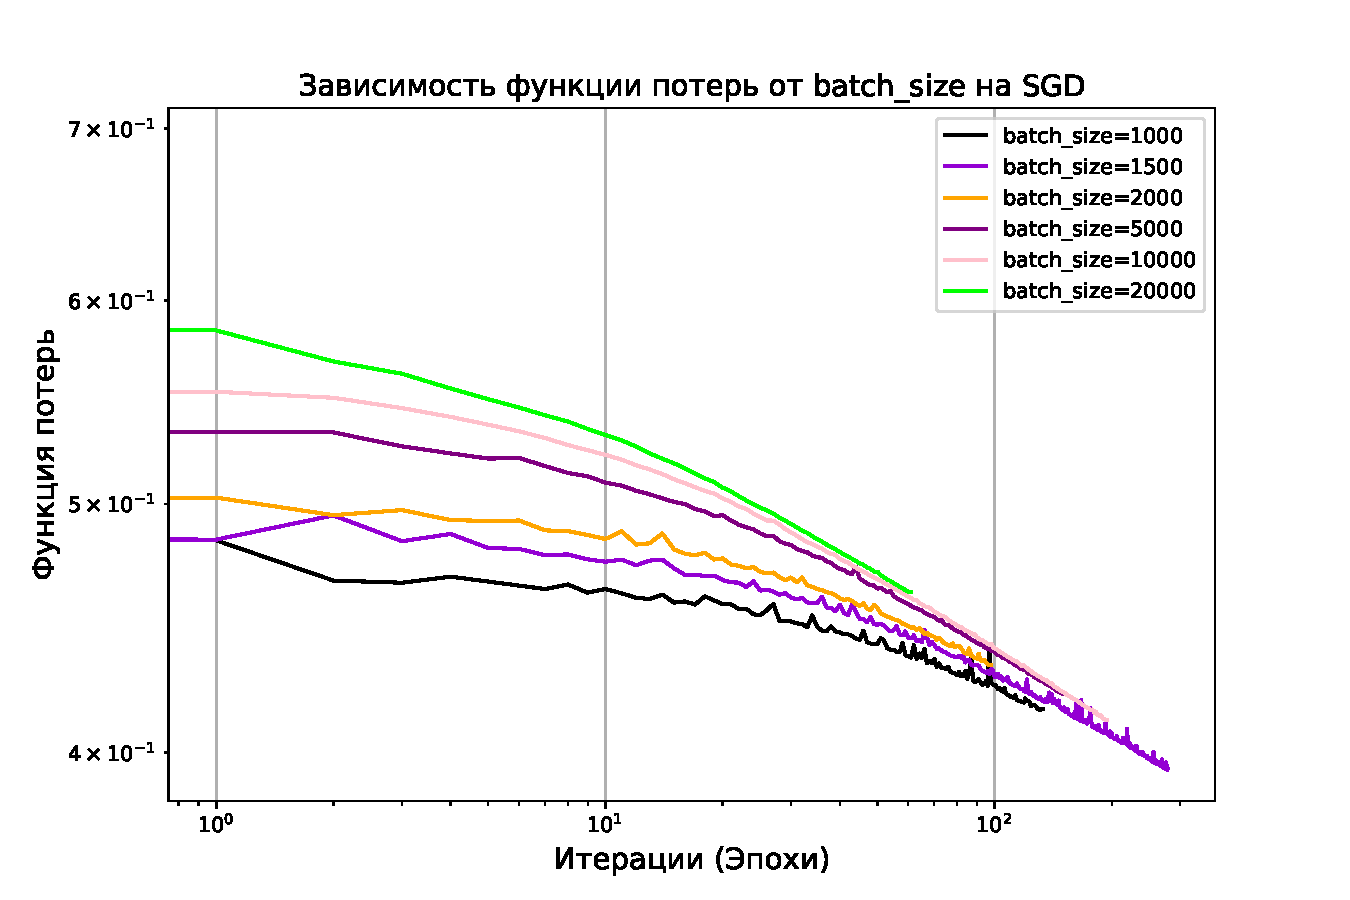
\includegraphics[width=0.7\linewidth]
    {exp_5_loss_batches_2.pdf}
    \caption{Значение функции потерь на эпохах модели в зависимости от параметра \textit{batch\_size}}
    \label{fig:exp_5_loss_batches_2}
\end{figure}

На рисунках \hyperref[fig:exp_5_loss_batches_1]{29} и \hyperref[fig:exp_5_loss_beta_2]{30} представлены графики зависимости значения функции потерь на каждой эпохе стохастического градиентного спуска от параметра \textit{batch\_size}. Как можно заметить из графиков, наилучшая сходимость значений функции потерь модели достигается при \textit{batch\_size = 300}.

\subsubsection{Подбор коэффициента $L_2$-регуляризации}

Будем рассматривать значения \textit{l2\_coef}, равномерно расположенные по логарифмической шкале от $ 10^{-4} $ до $ 10^{4} $.

\begin{figure}[H]
    \centering
    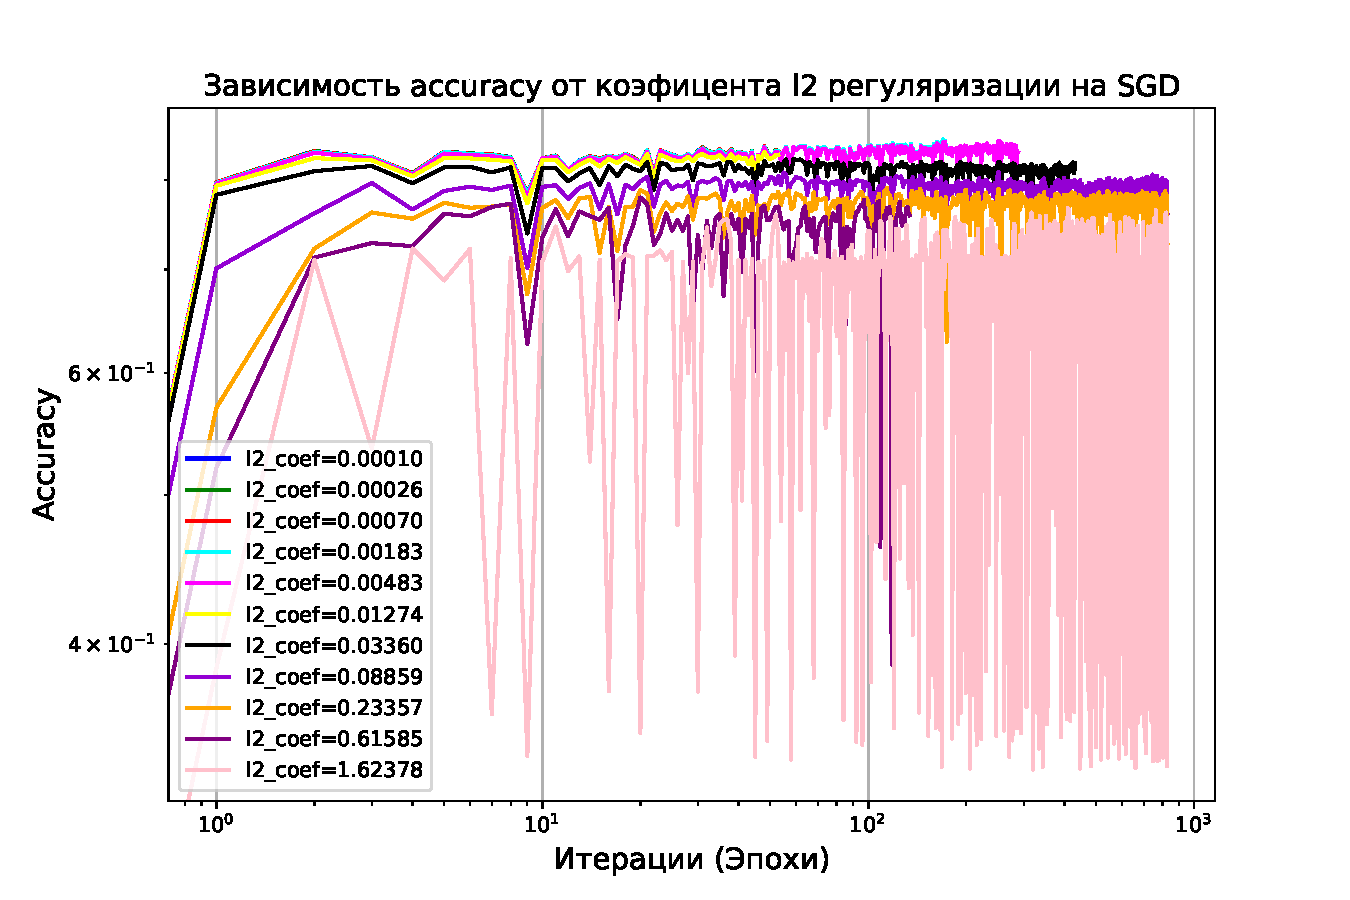
\includegraphics[width=0.7\linewidth]
    {exp_5_acc_l2_1.pdf}
    \caption{Accuracy на эпохах модели в зависимости от параметра \textit{l2\_coef}}
    \label{fig:exp_5_acc_l2_1}
\end{figure}

\begin{figure}[H]
    \centering
    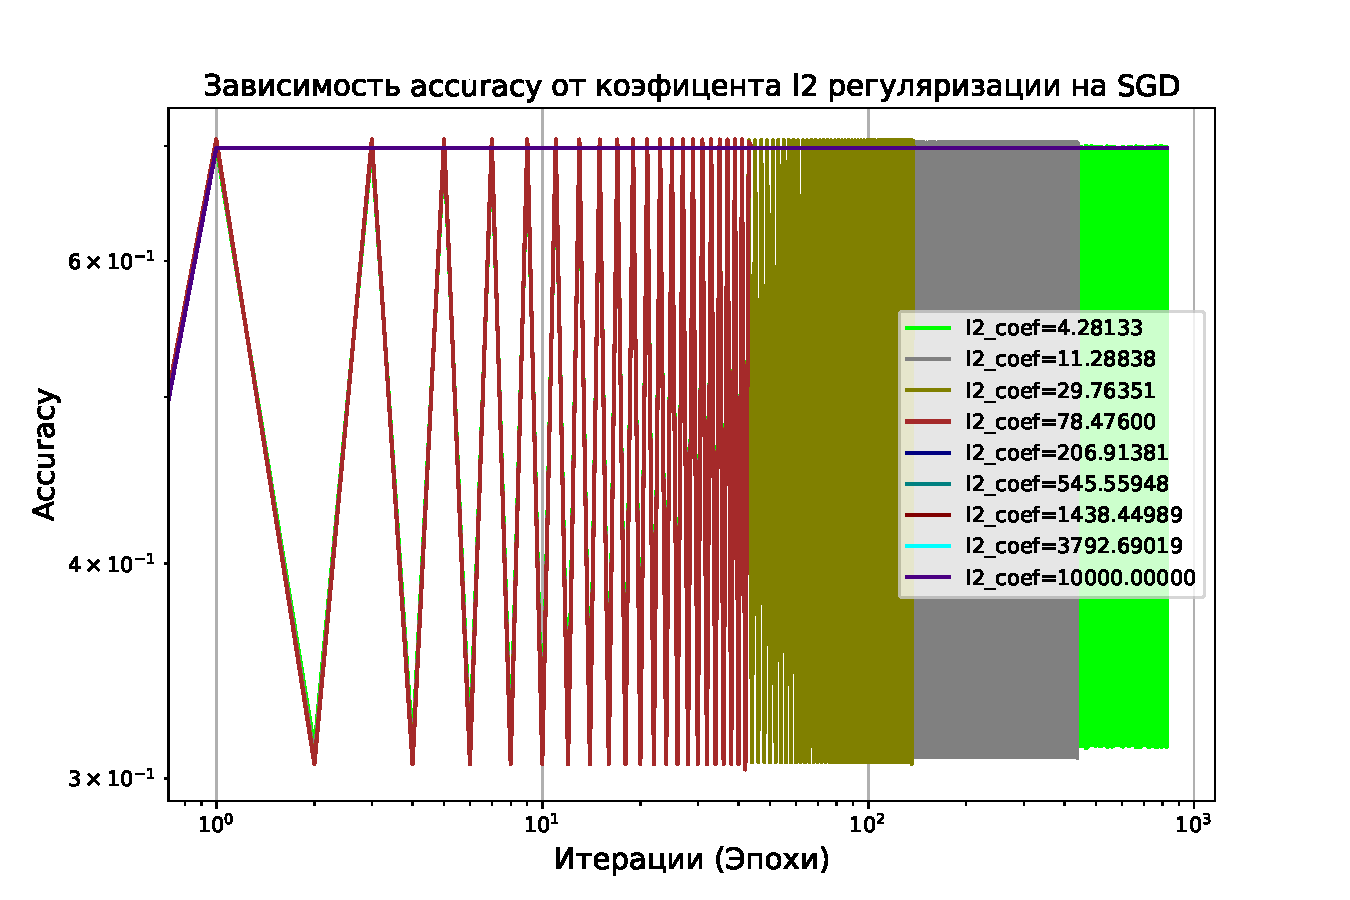
\includegraphics[width=0.7\linewidth]
    {exp_5_acc_l2_2.pdf}
    \caption{Accuracy на эпохах модели в зависимости от параметра \textit{l2\_coef}}
    \label{fig:exp_5_acc_l2_2}
\end{figure}

На рисунках \hyperref[fig:exp_5_acc_l2_1]{31} и \hyperref[fig:exp_5_acc_l2_2]{32} представлены графики зависимости accuracy модели на каждой эпохе стохастического градиентного спуска от параметра \textit{l2\_coef}. Как можно заметить из графиков, наилучшая точность модели достигается при \textit{l2\_coef = 0.00183298071}.

\begin{figure}[H]
    \centering
    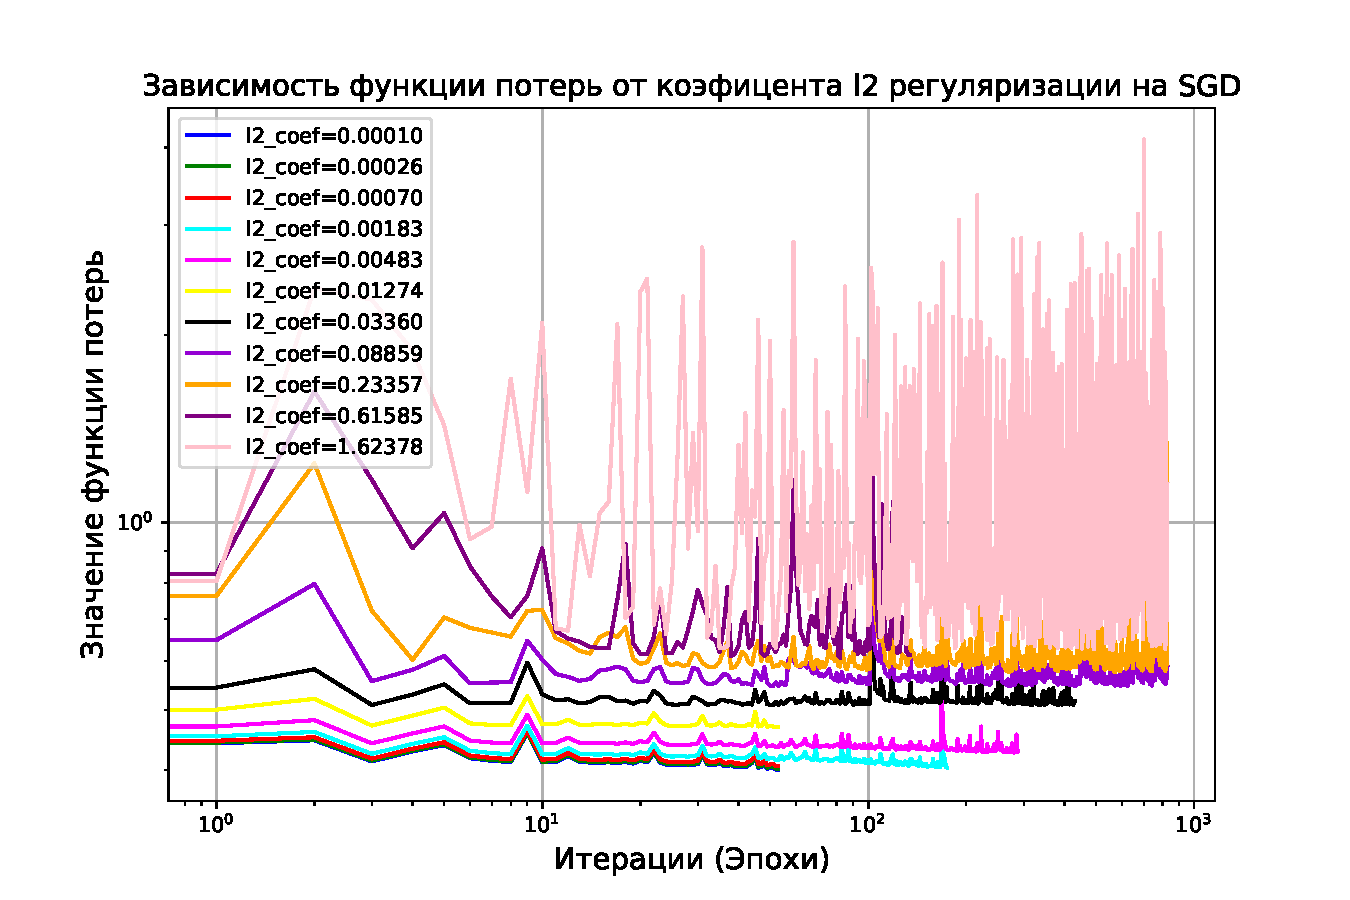
\includegraphics[width=0.7\linewidth]
    {exp_5_loss_l2_1.pdf}
    \caption{Значение функции потерь на эпохах модели в зависимости от параметра \textit{l2\_coef}}
    \label{fig:exp_5_loss_l2_1}
\end{figure}


На рисунке \hyperref[fig:exp_5_loss_l2_1]{33} представлены графики зависимости значения функции потерь на каждой эпохе стохастического градиентного спуска от параметра \textit{l2\_coef}. Как можно заметить из графиков, наилучшая сходимость значений функции потерь модели достигается при \textit{l2\_coef = 0.00183298071}.

\subsection{Выводы}
Проведенные эксперименты показали следующие лучшие параметры стохастического градиентного спуска для задачи логистической регрессии при прочих равных условиях:
\begin{itemize}
    \item \textit{step\_alpha = 0.372759372}
    \item \textit{step\_beta = 0.001}
    \item \textit{$ w_0 = (0, ... , 0)$}
    \item \textit{batch\_size = 300}
    \item \textit{l2\_coef = 0.00183298071}
\end{itemize}


\section{Сравнение градиентного и стохастического градиентного спуска для задачи логистической регрессии}

\subsection{Постановка задачи}

Сравнить поведение градиентного и стохастического градиентного спуска для задачи логистической регрессии.

\subsection{Реализация}

Обучим каждый метод на лучших параметрах, полученных в предыдущих разделах (\hyperref[sec:section5]{5} и \hyperref[sec:section5]{6}), и сравним их.

Рассмотрим accuracy и значения функции потерь на каждом шаге алгоритма метода, время работы каждой итерации (эпохи), а также общее время работы и итоговую точность.

\begin{figure}[H]
    \centering
    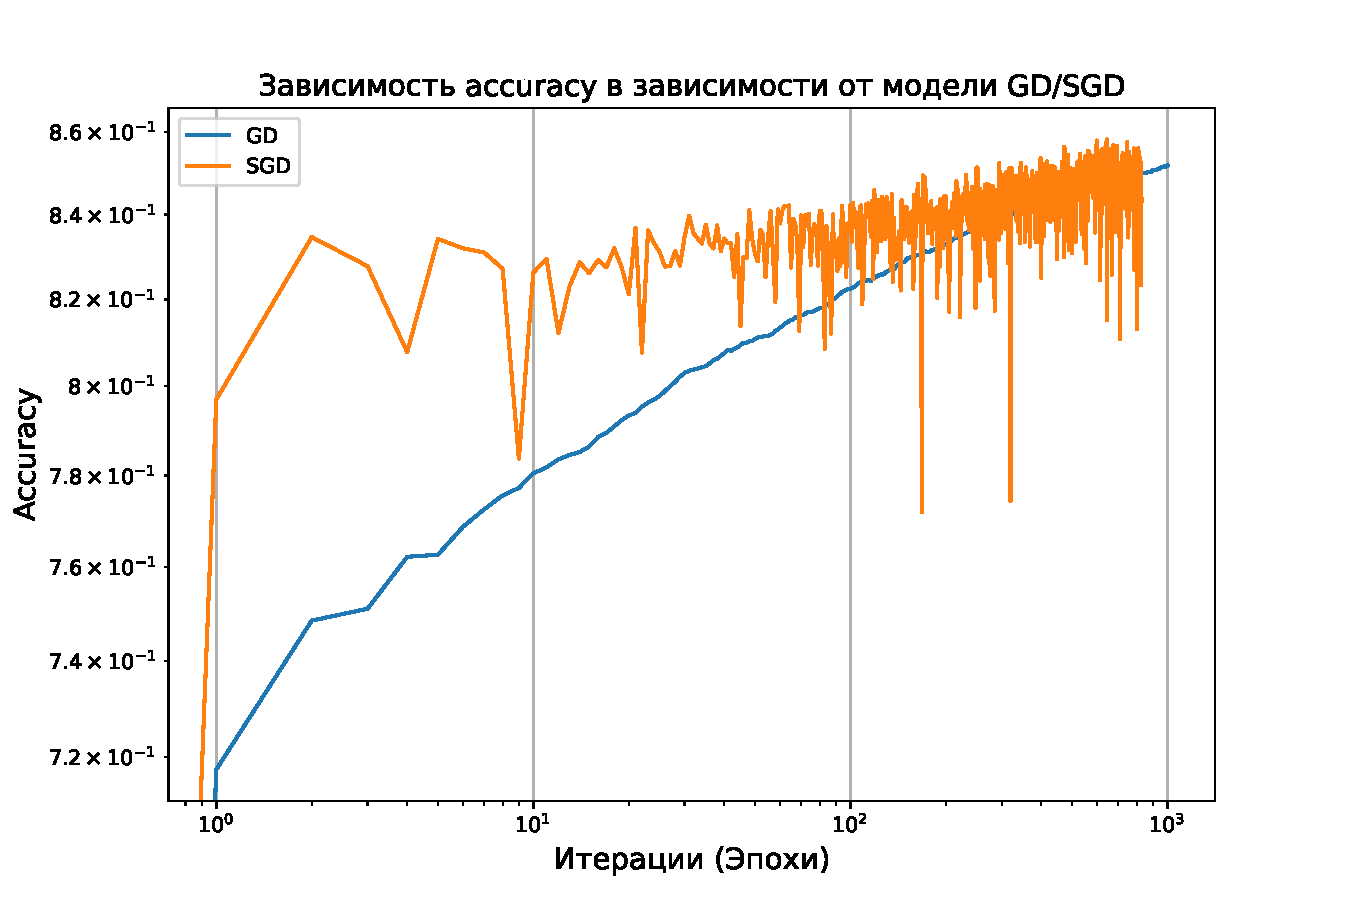
\includegraphics[width=0.7\linewidth]
    {exp_6_acc.pdf}
    \caption{Accuracy на итерациях (эпохах) методов GD/SGD}
    \label{fig:exp_6_acc}
\end{figure}

\begin{figure}[H]
    \centering
    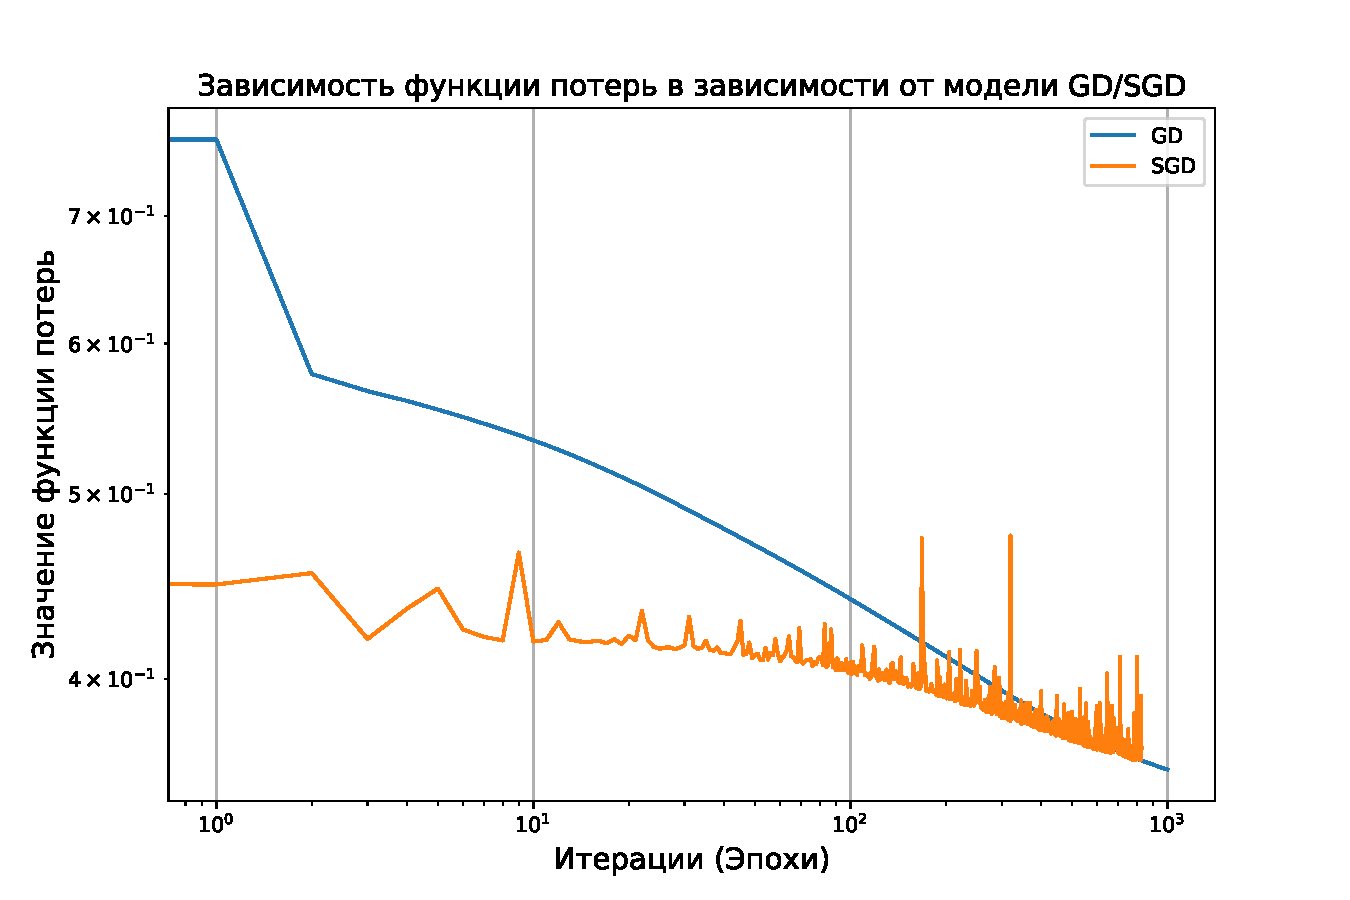
\includegraphics[width=0.7\linewidth]
    {exp_6_loss.pdf}
    \caption{Значения функции потерь на итерациях (эпохах) методов GD/SGD}
    \label{fig:exp_6_loss}
\end{figure}

На рисунках \hyperref[fig:exp_6_acc]{34} и \hyperref[fig:exp_6_loss]{35} представлены графики зависимости accuracy и значения функции потерь на каждой итерации (эпохе) градиентного и  стохастического градиентного спуска. Как можно заметить из графиков, метод градиентного спуска дает лучшую точность, однако, значение функции потерь сходится быстрее на методе стохастического градиентного спуска.

\begin{figure}[H]
    \centering
    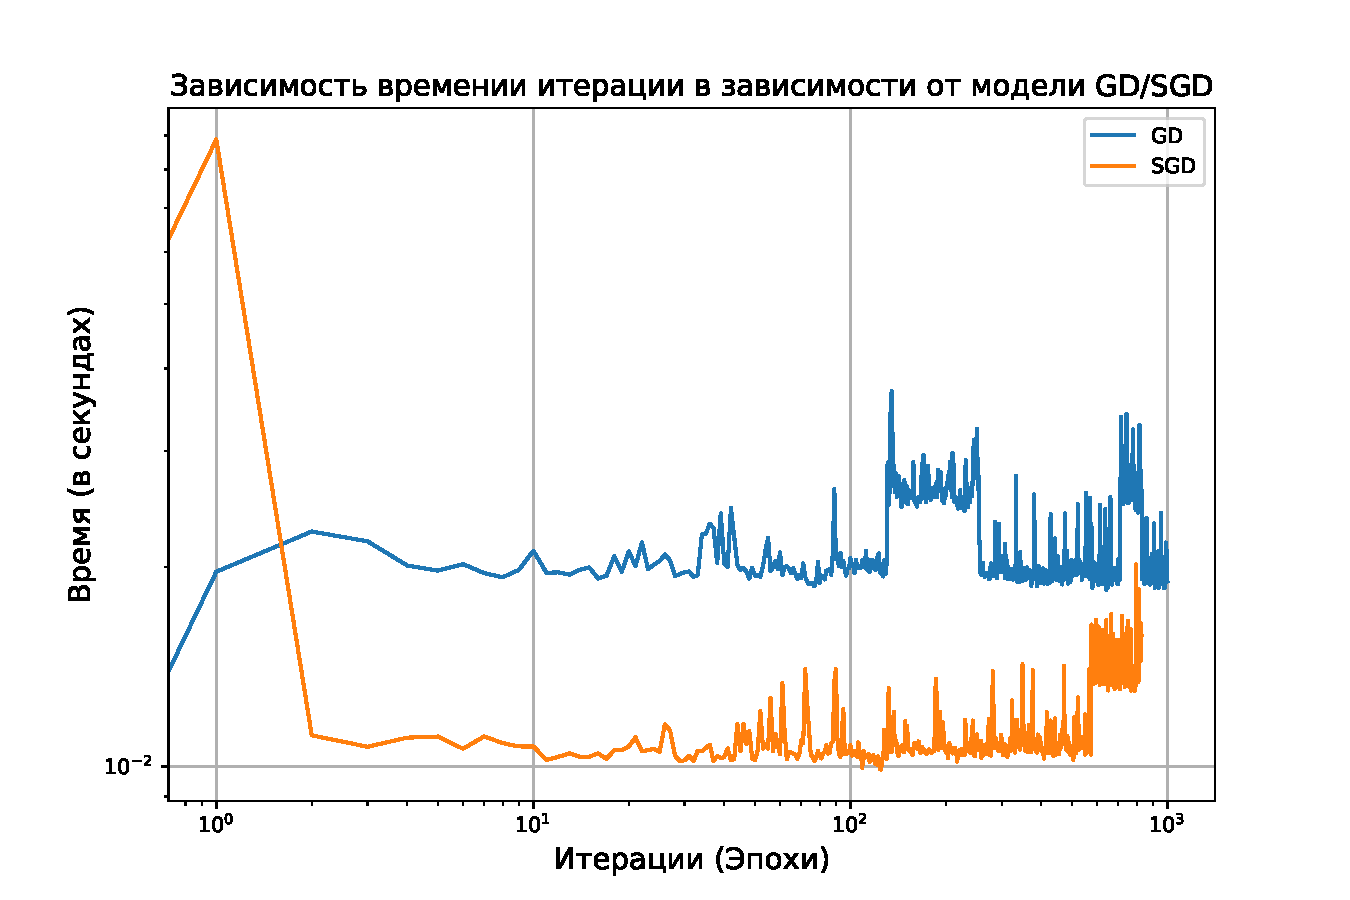
\includegraphics[width=0.7\linewidth]
    {exp_6_time.pdf}
    \caption{Время работы итераций (эпох) методов GD/SGD}
    \label{fig:exp_6_time}
\end{figure}

На рисунке \hyperref[fig:exp_6_acc]{36} представлен время работы итераций (эпох) методов градиентного и стохастического градиентного спуска. Как можно заметить из графиков, метод стохастического градиентного спуска затрачивает на одну эпоху меньше времени, чем метод градиентного спуска на одну итерацию.

В таблице \hyperref[tab:exp_6_acc_time]{1} ниже представлены точности на тестовой выборке и общее время работы методов градиентного и стохастического градиентного спуска. Как можно заметить из таблицы, стохастичесский работает в разы быстрее градиентного спуска, причем accuracy двух методов отличается не больше, чем на $10^{-2}$ .

\begin{table}[H]
    \centering
    \begin{tabular}{|l|c|c|}
        \hline
        Метод & Accuracy & Время выполнения(сек.) \\ \hline
        \textit{GD} & 0.851760495260205 & 21.50232481956482 \\ \hline
        \textit{SGD} & 0.8435867672663958 & 9.866184711456299 \\ \hline
    \end{tabular}
    \caption{Точность на тестовой выборке и общее время работы методов градиентного и стохастического градиентного спуска}
    \label{tab:exp_6_acc_time}
\end{table}

\subsection{Выводы}

Анализ представленных данных показывает, что выбор между методом градиентного и стохастического градиентного спуска зависит от приоритетов решаемой задачи:

\begin{itemize}
    \item Градиентный спуск демонстрирует лучшую точность, что может быть критически важным для задач, где даже небольшое улучшение точности играет значимую роль.
    \item Стохастический градиентный спуск обеспечивает более быстрое время сходимости функции потерь и значительно снижает затраты по времени, что делает его предпочтительным для задач, где вычислительные ресурсы ограничены или требуется быстрая обработка больших объемов данных.
\end{itemize}

Таким образом, если точность критична, предпочтителен градиентный спуск, однако, если важнее время обработки и ресурсоёмкость, более эффективным будет стохастический градиентный спуск. Отличие между точностями обоих методов минимально (менее \(10^{-2}\)), что делает стохастический метод более практичным для большинства задач.

\section{Лемматизация}

\subsection{Постановка задачи}

Применить алгоритм лемматизации \textit{WordNetLemmatizer} из библиотеки \textit{nltk} к коллекции комментариев. Удалить из текста стоп-слова, используя список стоп-слов из \textit{nltk}. Исследовать, как предобработка корпуса повлияла на точность классификации, время работы алгоритма и размерность признакового пространства.

\subsection{Реализация}
Произведем лемматизацию текстов комментариев, используя класс \\ \textit{WordNetLemmatizer}. В процессе лемматизации удаляются стоп-слова — слова и символы, которые не несут значимой смысловой нагрузки. Остальные слова преобразуются в их начальную форму, т.е. в инфинитив.

Сравним размерности признакового пространства выборки до и после лемматизации:

\begin{table}[H]
    \centering
    \begin{tabular}{|l|c|c|}
        \hline
        Выборка & Размерность признакового пространства \\ \hline
        \textit{До лемматизации} & 3736 \\ \hline
        \textit{После лемматизации} & 3195 \\ \hline
    \end{tabular}
    \caption{Размерность признакового пространства выборки до и после лемматизации}
    \label{tab:exp_7_lemm_dim}
\end{table}

В таблице \hyperref[tab:exp_7_lemm_dim]{2} приведены размерности признакового пространства выборки до и после лемматизации. Как можно заметить из таблицы, лемматизация позволила сократить признаковое пространство на 541 признак.

Рассмотрим, как проведение лемматизации повлияло на изменение точности, значения функции потерь на каждой итерации (эпохе), а также времени ее выполнения.

\begin{figure}[H]
    \centering
    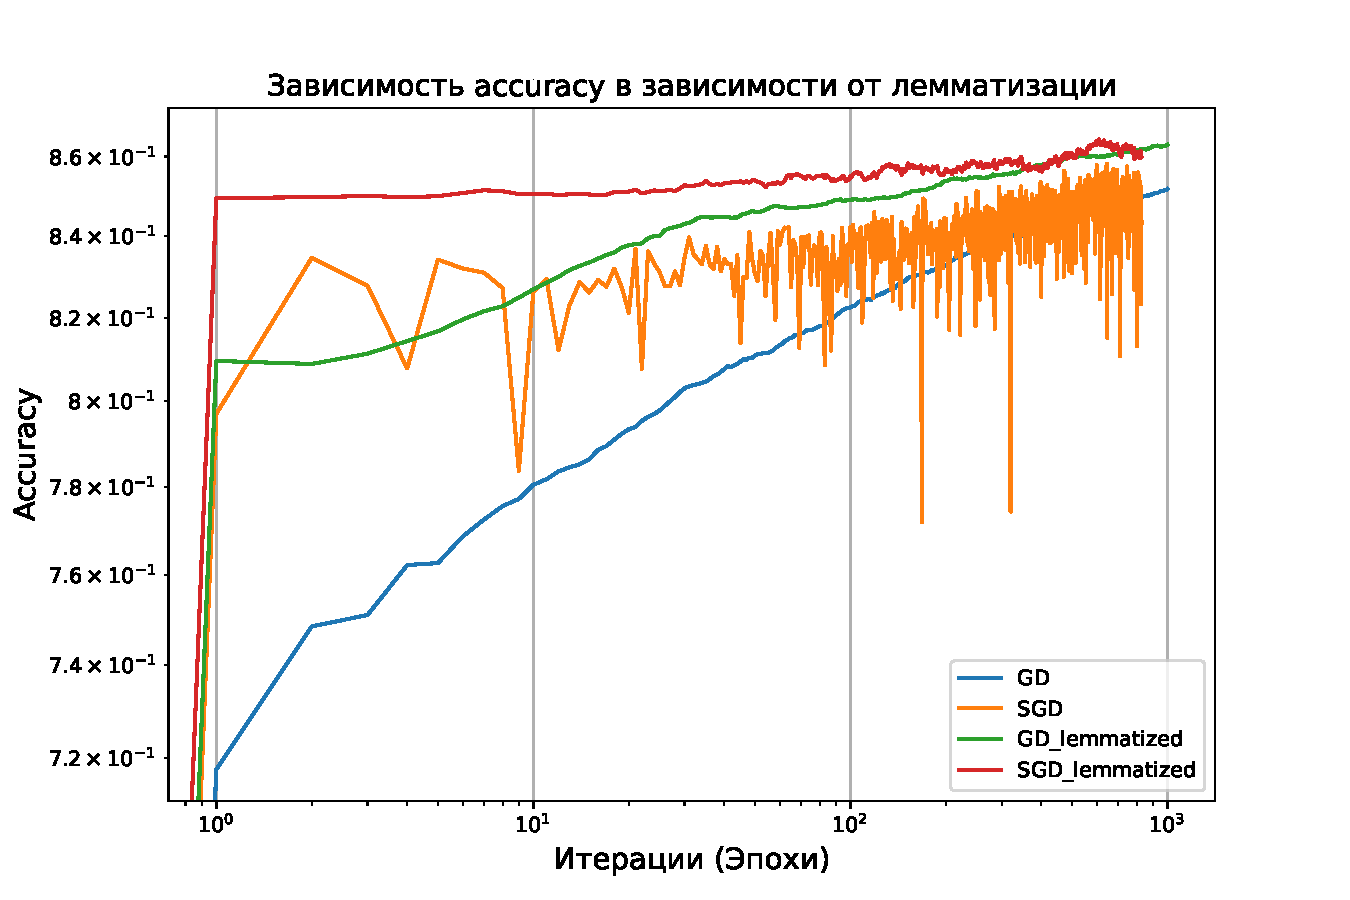
\includegraphics[width=0.7\linewidth]
    {exp_7_acc.pdf}
    \caption{Accuracy на итерациях (эпохах) методов GD/SGD в зависимости от проведения лемматизации}
    \label{fig:exp_7_acc}
\end{figure}

\begin{figure}[H]
    \centering
    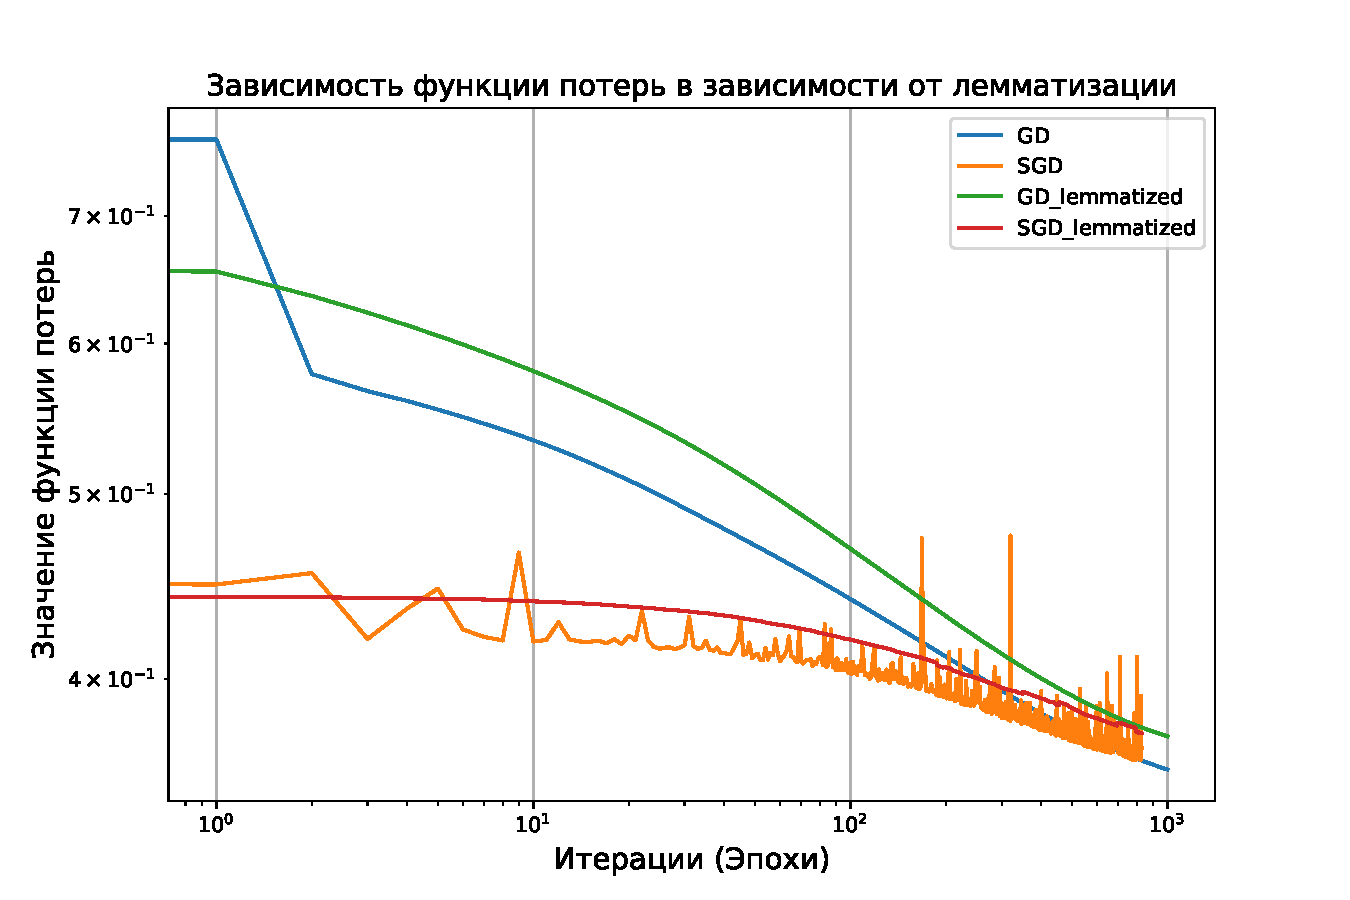
\includegraphics[width=0.7\linewidth]
    {exp_7_loss.pdf}
    \caption{Значения функции потерь на итерациях (эпохах) методов GD/SGD в зависимости от проведения лемматизации}
    \label{fig:exp_7_loss}
\end{figure}

На рисунках \hyperref[fig:exp_7_acc]{37} и \hyperref[fig:exp_7_loss]{38} представлены графики зависимости accuracy и значения функции потерь на каждой итерации (эпохе) градиентного и  стохастического градиентного спуска от проведения лемматизации. Как можно заметить из графиков, лемматизация улучшает эффективность обоих методов, повышая accuracy с первых итераций (эпох) методов и ускоряя сходимость функции потерь. Метод стохастического градиентного спуска показывает на лемматизированной выборке намного больше стабильность.

В таблице \hyperref[tab:exp_6_acc_time]{3} ниже представлены точности на тестовой выборке и общее время работы методов градиентного и стохастического градиентного спуска в зависимости от проведения лемматизации.

\begin{table}[H]
    \centering
    \begin{tabular}{|l|c|c|}
        \hline
        Метод & Accuracy & Время выполнения(сек.) \\ \hline
        \textit{GD} & 0.851760495260205 & 21.50232481956482 \\ \hline
        \textit{SGD} & 0.8435867672663958 & 9.866184711456299 \\ \hline
        \textit{GD\_lemmatized} & 0.8630295995356936 & 27.30692982673645 \\ \hline
        \textit{SGD\_lemmatized} & 0.8599825885084156 & 10.892971515655518 \\ \hline
    \end{tabular}
    \caption{Точность на тестовой выборке и общее время работы методов градиентного и стохастического градиентного спуска в зависимости от проведения лемматизации}
    \label{tab:exp_7_acc_time}
\end{table}

Исходя из вышеприведенных данных, лемматизация улучшает точность обоих методов, однако требует увеличения времени выполнения. Метод GD показывает лучшую точность после лемматизации, тогда как SGD сохраняет преимущество в скорости работы.

\subsection{Выводы}

Лемматизация положительно сказывается на эффективности обоих методов, улучшая accuracy с первых итераций и ускоряя сходимость функции потерь. Несмотря на увеличение времени выполнения, её применение обеспечивает значительное повышение стабильности метода SGD и улучшение итоговой точности для метода GD.

\section{Сравнение представлений \textit{BagOfWords} и \textit{Tfidf} и подбор параметров \textit{min\_df} и \textit{max\_df} конструкторов}

\subsection{Постановка задачи}

Исследовать качество, время работы алгоритма и размер признакового пространства в зависимости от следующих факторов:

\begin{itemize}
    \item использовалось представление \textit{BagOfWords} или \textit{Tfidf}
    \item параметров \textit{min\_df} и \textit{max\_df} конструкторов.
\end{itemize}

\subsection{Реализация}

Для построения представлений \textit{BagOfWords} и \textit{Tfidf} использовались \textit{CountVectorizer} и \textit{TfidfVectorizer} из библиотеки \textit{sklearn}, соответственно.

\subsubsection{Сравнение представлений \textit{BagOfWords} и \textit{Tfidf} с параметрами по умолчанию}

Построим представления \textit{BagOfWords} и \textit{Tfidf} с параметрами по умолчанию. Сравним точность, значения функции потерь на каждой итерации (эпохе), а также время ее выполнения в зависимости от представления. В сравнении использовались модели с ранее подобранными лучшими параметрами.

\begin{figure}[H]
    \centering
    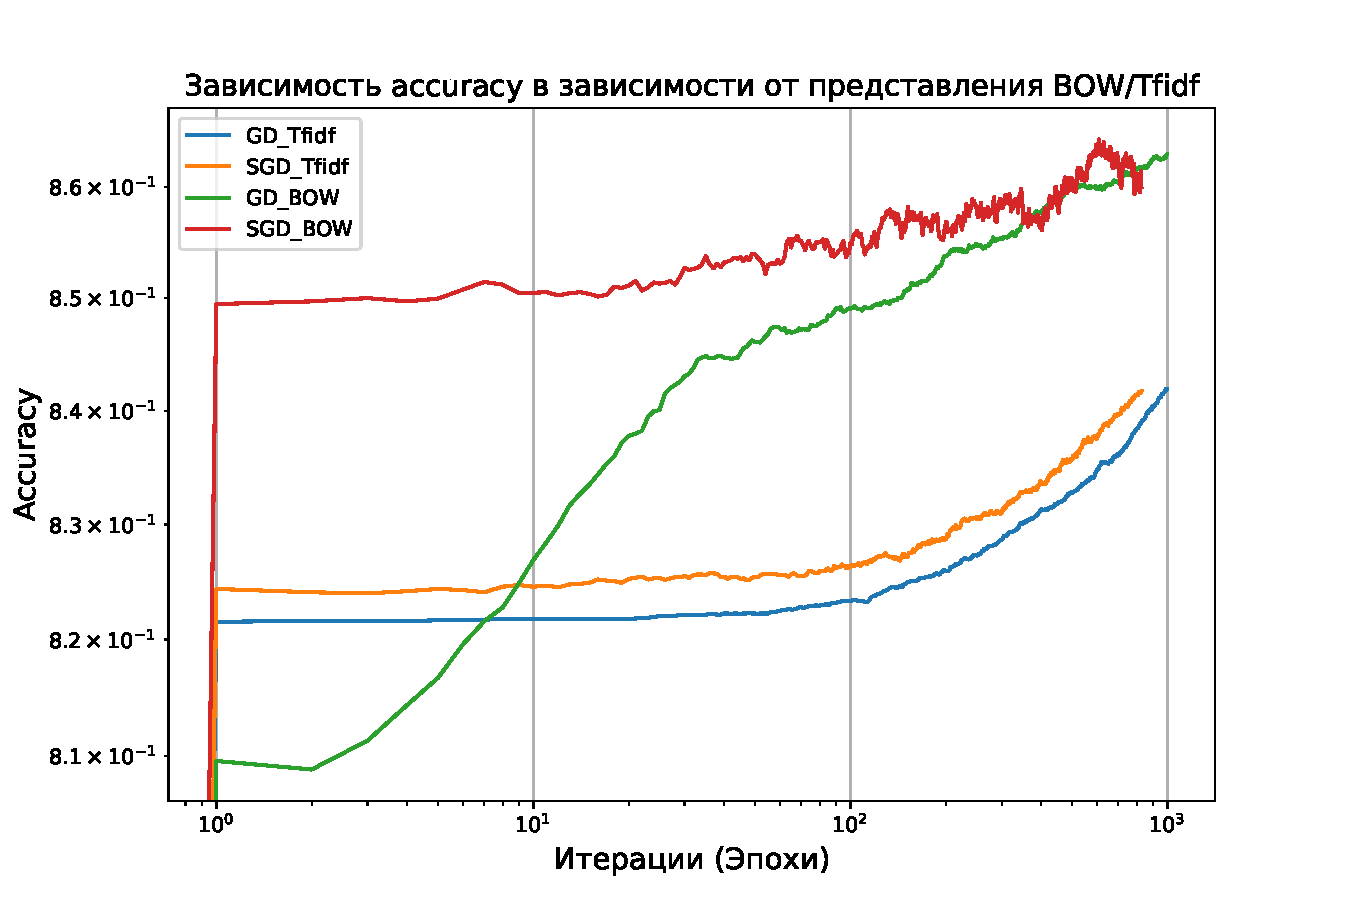
\includegraphics[width=0.7\linewidth]
    {exp_8_acc.pdf}
    \caption{Accuracy на итерациях (эпохах) методов GD/SGD в зависимости от представления \textit{BOW/Tfidf}}
    \label{fig:exp_8_acc}
\end{figure}

\begin{figure}[H]
    \centering
    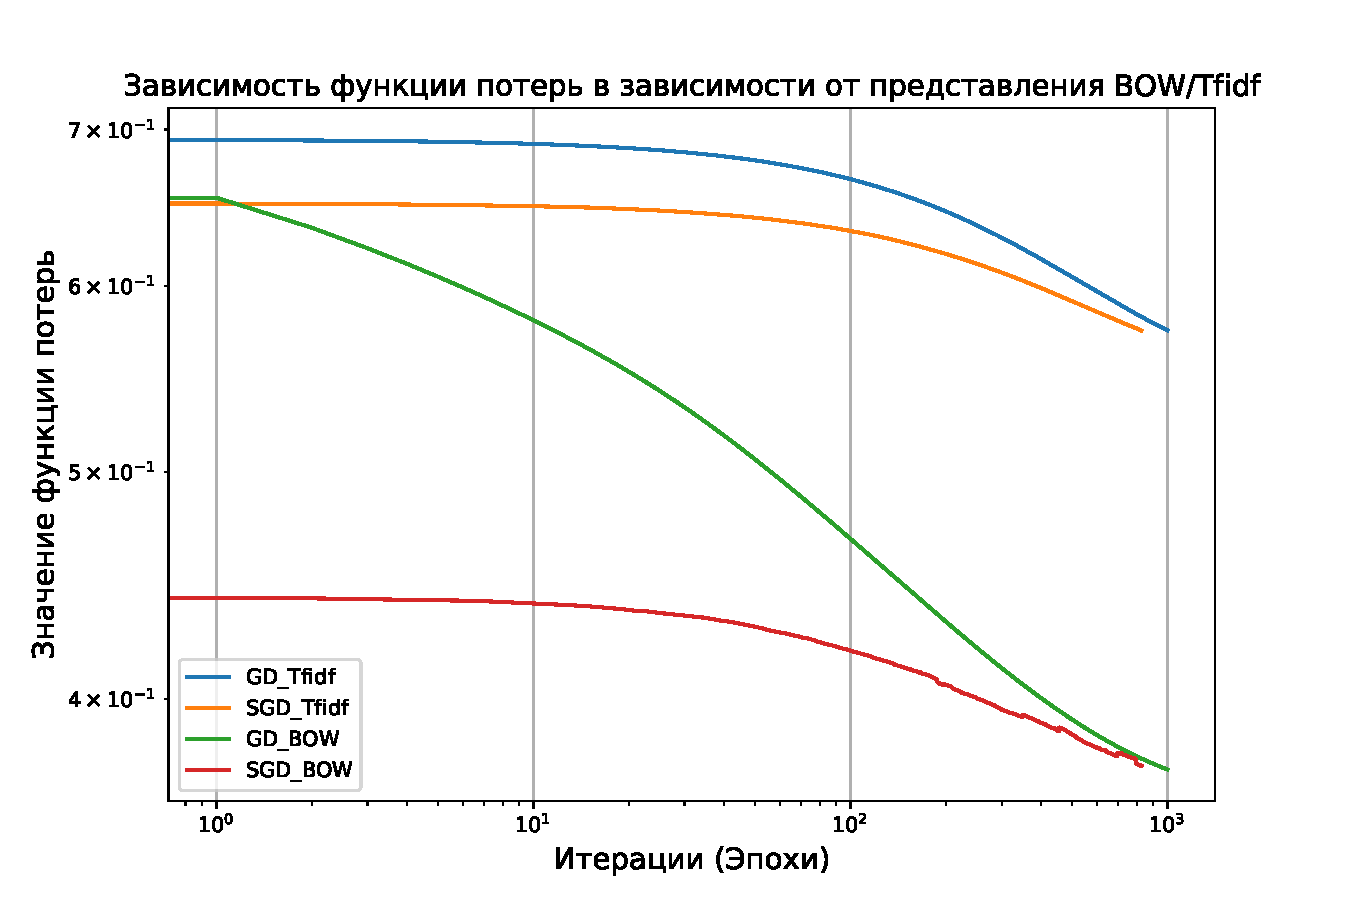
\includegraphics[width=0.7\linewidth]
    {exp_8_loss.pdf}
    \caption{Значения функции потерь на итерациях (эпохах) методов GD/SGD в зависимости от представления \textit{BOW/Tfidf}}
    \label{fig:exp_8_loss}
\end{figure}

На рисунках \hyperref[fig:exp_8_acc]{39} и \hyperref[fig:exp_8_loss]{40} представлены графики зависимости accuracy и значения функции потерь на каждой итерации (эпохе) градиентного и  стохастического градиентного спуска от представления \textit{BOW/Tfidf}. Как можно заметить из графиков, представление \textit{BOW} улучшает точность и ускоряет сходимость функции потерь для методов GD и SGD, делая \textit{BOW} предпочтительным выбором по сравнению с \textit{Tfidf}.

В таблице \hyperref[tab:exp_6_acc_time]{4} ниже представлены точности на тестовой выборке и общее время работы методов градиентного и стохастического градиентного спуска в зависимости от представления \textit{BOW/Tfidf}.

\begin{table}[H]
    \centering
    \begin{tabular}{|l|c|c|}
        \hline
        Метод & Accuracy & Время выполнения(сек.) \\ \hline
        \textit{GD\_Tfidf} & 0.8418939833623524 & 12.866596937179565 \\ \hline
        \textit{SGD\_Tfidf} & 0.8417488875991488 & 5.978341341018677 \\ \hline
        \textit{GD\_BOW} & 0.8630295995356936 & 27.30692982673645 \\ \hline
        \textit{SGD\_BOW} & 0.8599825885084156 & 10.892971515655518 \\ \hline
    \end{tabular}
    \caption{Точность на тестовой выборке и общее время работы методов градиентного и стохастического градиентного спуска в зависимости от представления \textit{BOW/Tfidf}}
    \label{tab:exp_8_acc_time}
\end{table}

Исходя из вышеприведенных данных, представление \textit{BOW} обеспечивает более высокую точность, но требует больше времени выполнения, а \textit{Tfidf} позволяет значительно ускорить работу методов, но с небольшим снижением точности.

\subsubsection{Сравнение представлений \textit{BOW/Tfidf} по параметрам \textit{min\_df} и \textit{max\_df} конструкторов}

Сравним работу моделей по параметрам \textit{min\_df} и \textit{max\_df} конструкторов представлений \textit{BOW/Tfidf}.

Будем рассматривать параметры \textit{min\_df}, равномерно расположенные по логарифмической шкале от $ 10^{-10} $ до $ 10^{-1} $, а также проанализируем параметры \textit{max\_df}, равномерно расположенные по линейной шкале от 0.4 до 1.

\begin{figure}[H]
    \centering
    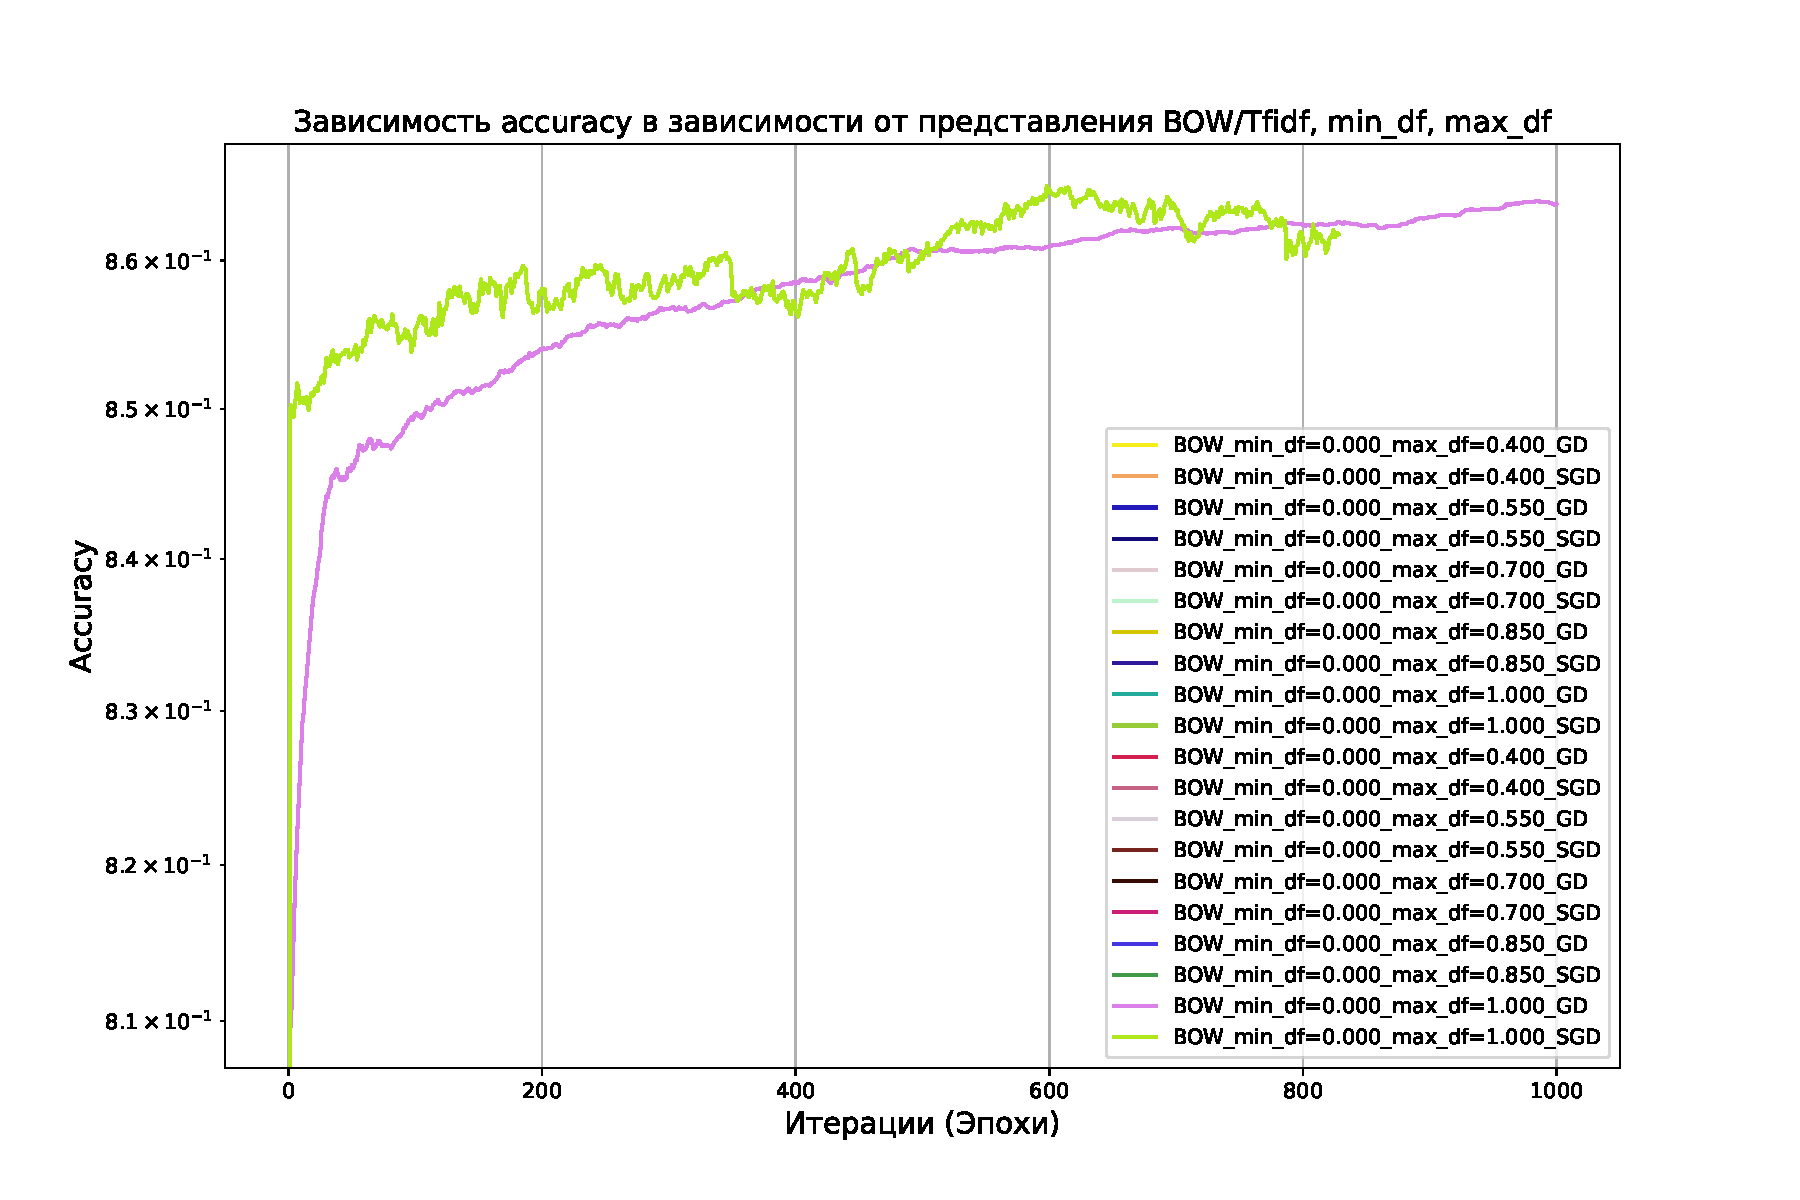
\includegraphics[width=0.85\linewidth]
    {exp_8_min_max_df_acc_1.pdf}
    \caption{Accuracy на итерациях (эпохах) методов GD/SGD в зависимости от представления \textit{BOW/Tfidf} и параметров \textit{min\_df} и \textit{max\_df}}
    \label{fig:exp_8_min_max_df_acc_1}
\end{figure}

\begin{figure}[H]
    \centering
    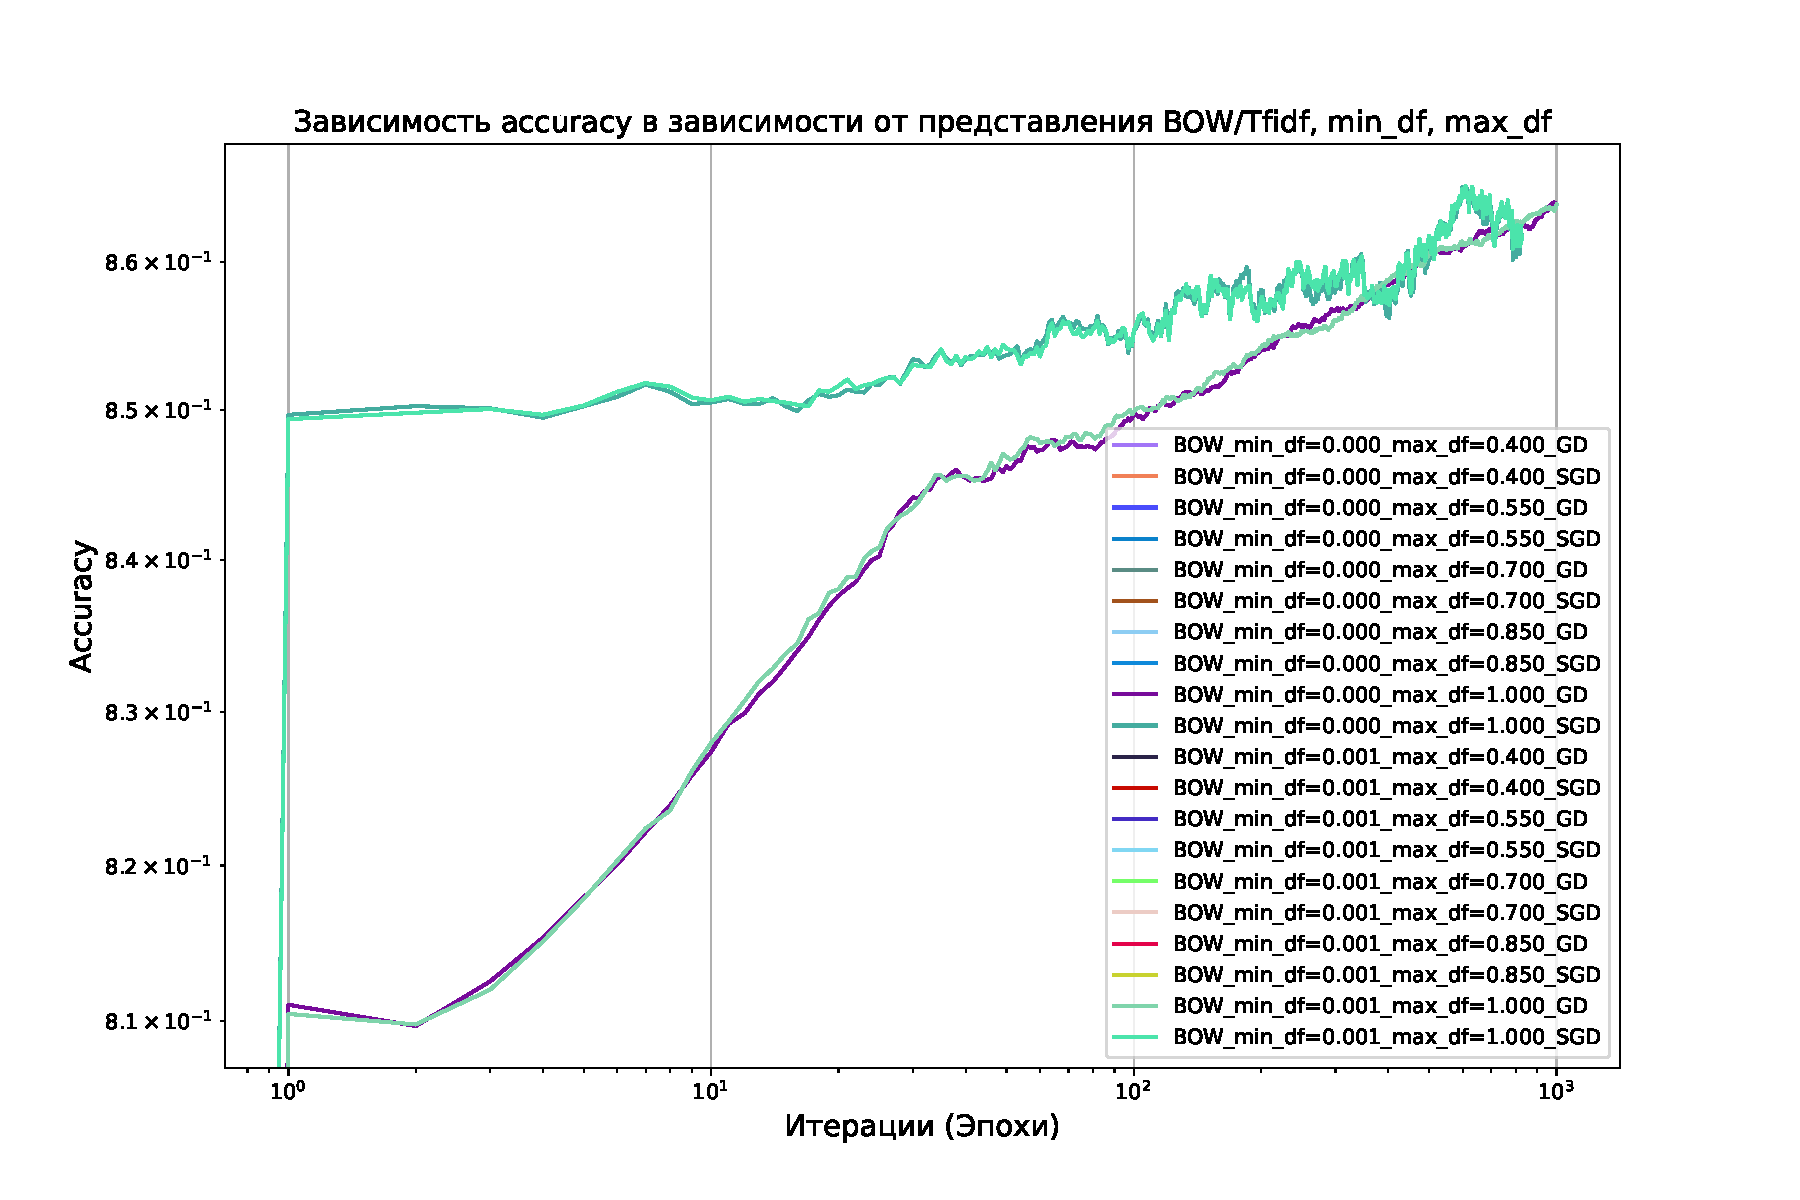
\includegraphics[width=0.85\linewidth]
    {exp_8_min_max_df_acc_2.pdf}
    \caption{Accuracy на итерациях (эпохах) методов GD/SGD в зависимости от представления \textit{BOW/Tfidf} и параметров \textit{min\_df} и \textit{max\_df}}
    \label{fig:exp_8_min_max_df_acc_2}
\end{figure}

\begin{figure}[H]
    \centering
    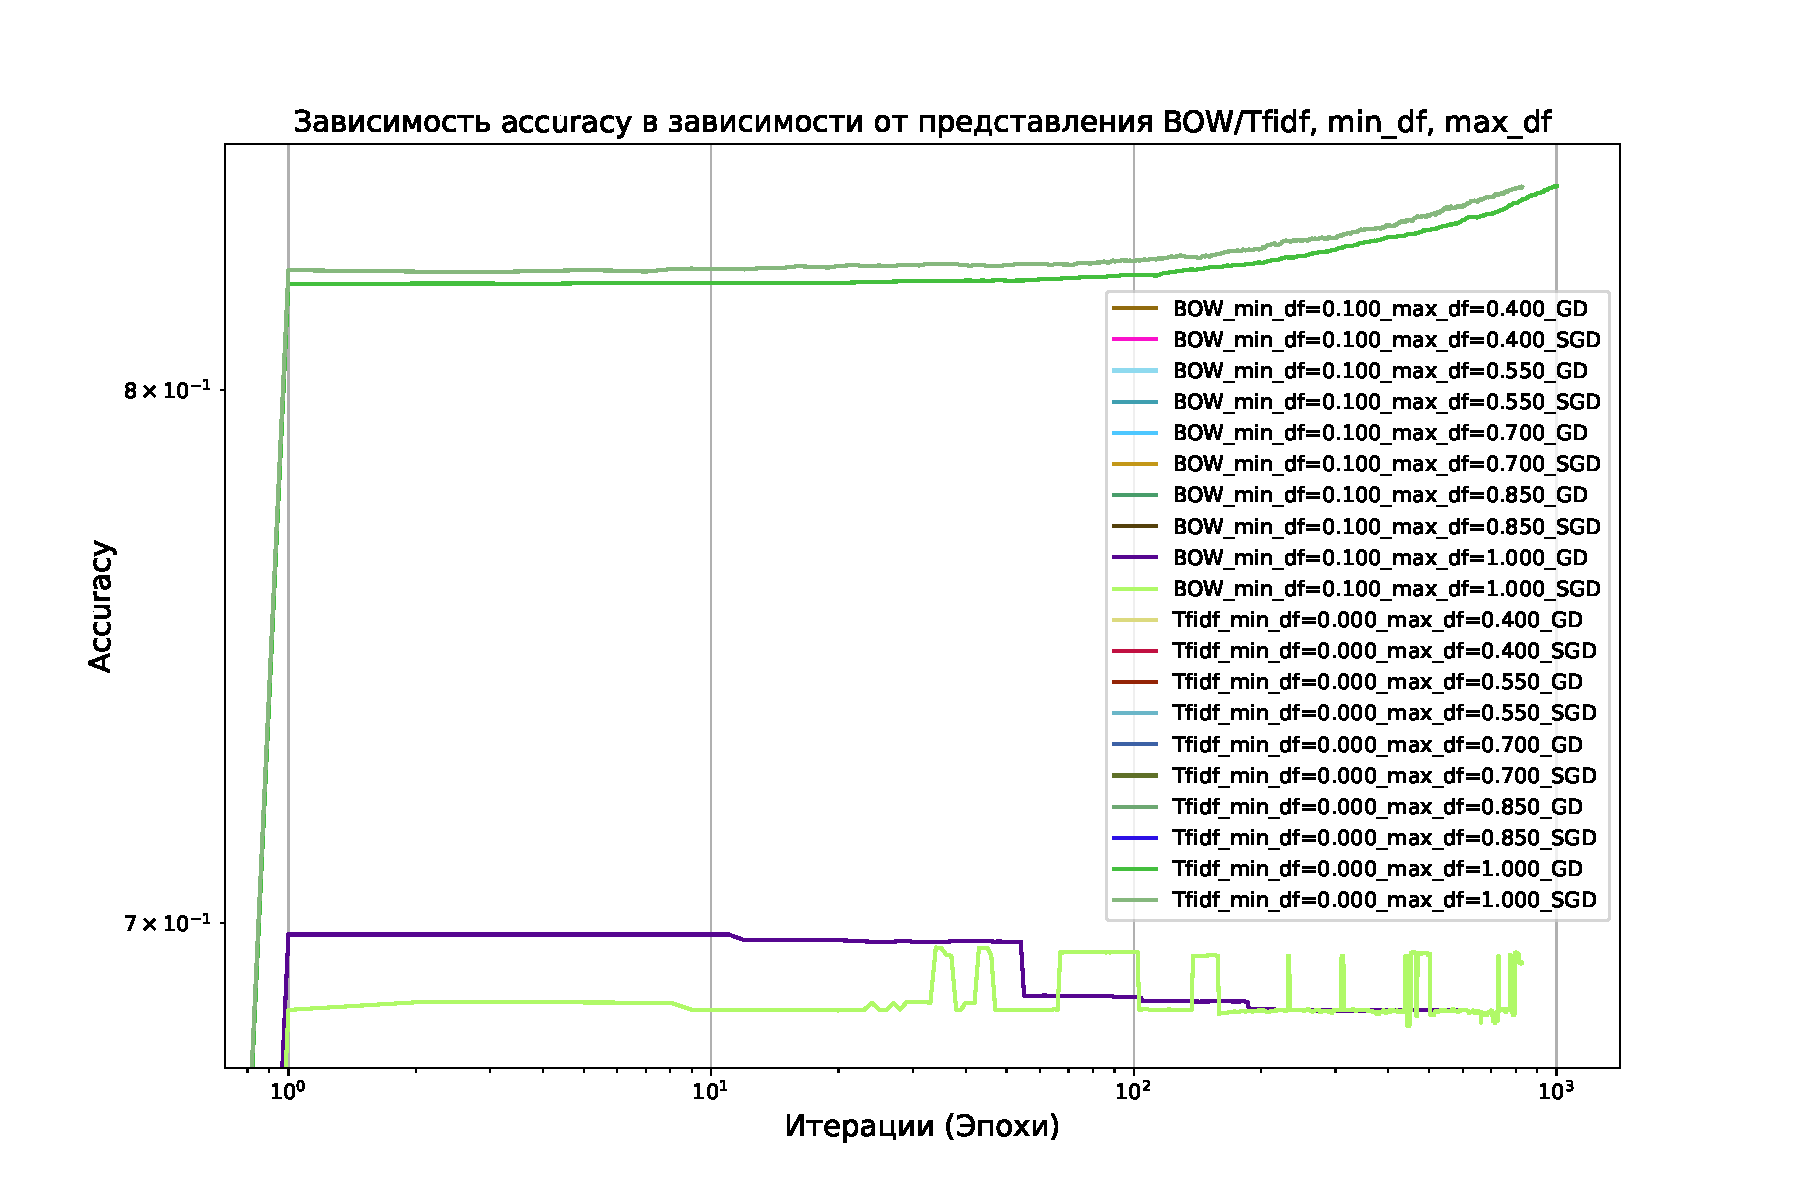
\includegraphics[width=0.85\linewidth]
    {exp_8_min_max_df_acc_3.pdf}
    \caption{Accuracy на итерациях (эпохах) методов GD/SGD в зависимости от представления \textit{BOW/Tfidf} и параметров \textit{min\_df} и \textit{max\_df}}
    \label{fig:exp_8_min_max_df_acc_3}
\end{figure}

\begin{figure}[H]
    \centering
    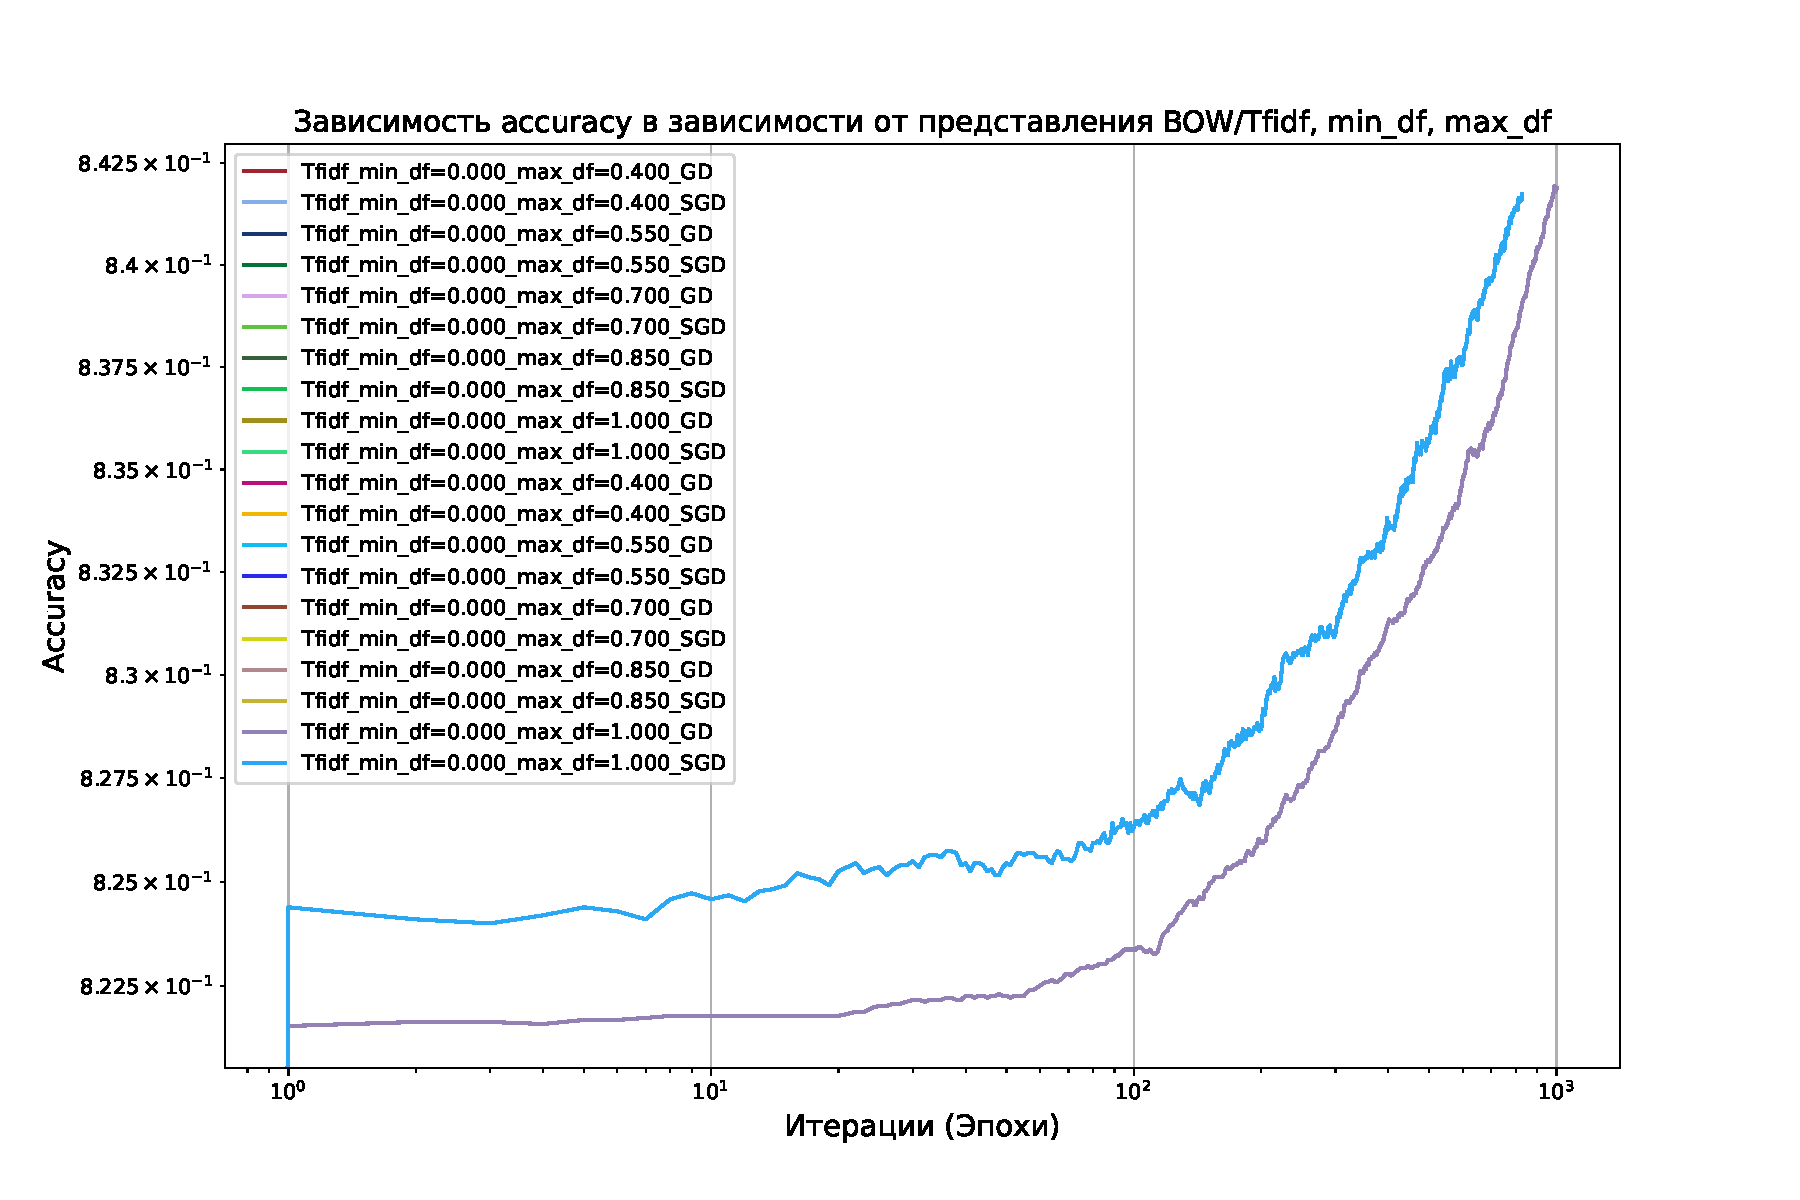
\includegraphics[width=0.85\linewidth]
    {exp_8_min_max_df_acc_4.pdf}
    \caption{Accuracy на итерациях (эпохах) методов GD/SGD в зависимости от представления \textit{BOW/Tfidf} и параметров \textit{min\_df} и \textit{max\_df}}
    \label{fig:exp_8_min_max_df_acc_4}
\end{figure}

\begin{figure}[H]
    \centering
    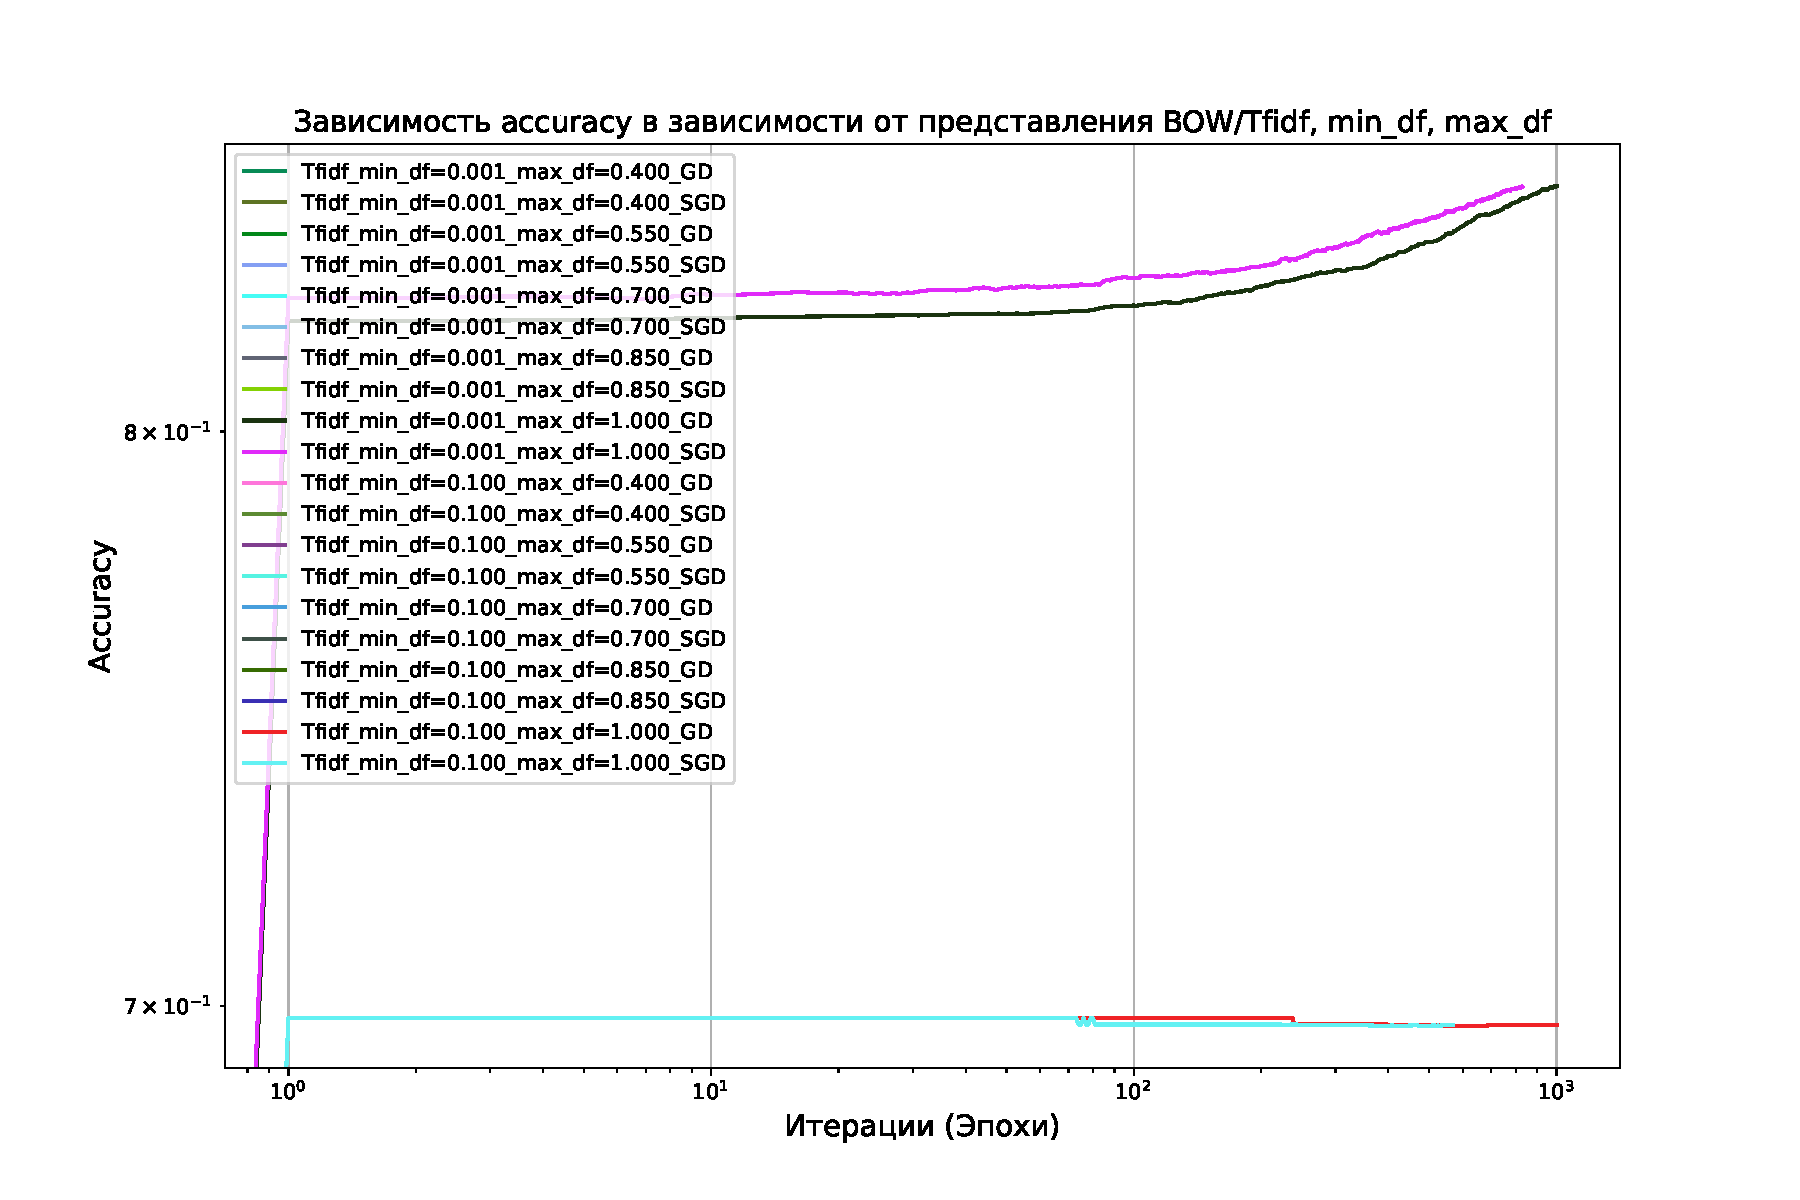
\includegraphics[width=0.85\linewidth]
    {exp_8_min_max_df_acc_5.pdf}
    \caption{Accuracy на итерациях (эпохах) методов GD/SGD в зависимости от представления \textit{BOW/Tfidf} и параметров \textit{min\_df} и \textit{max\_df}}
    \label{fig:exp_8_min_max_df_acc_5}
\end{figure}

На рисунках \hyperref[fig:exp_8_min_max_df_acc_1]{41}, \hyperref[fig:exp_8_min_max_df_acc_2]{42}, \hyperref[fig:exp_8_min_max_df_acc_3]{43}, \hyperref[fig:exp_8_min_max_df_acc_4]{44}, \hyperref[fig:exp_8_min_max_df_acc_5]{45} представлены графики зависимости accuracy на каждой итерации (эпохе) градиентного и стохастического градиентного спуска от представления \textit{BOW/Tfidf} и параметров \textit{min\_df} и \textit{max\_df}. Как можно заметить из графиков, увеличение параметра \textit{min\_df} или уменьшение \textit{max\_df} приводит к стабилизации и улучшению результатов. Более строгие ограничения на частотность позволяют исключить незначимые признаки, что ускоряет сходимость и повышает итоговую точность.

\begin{figure}[H]
    \centering
    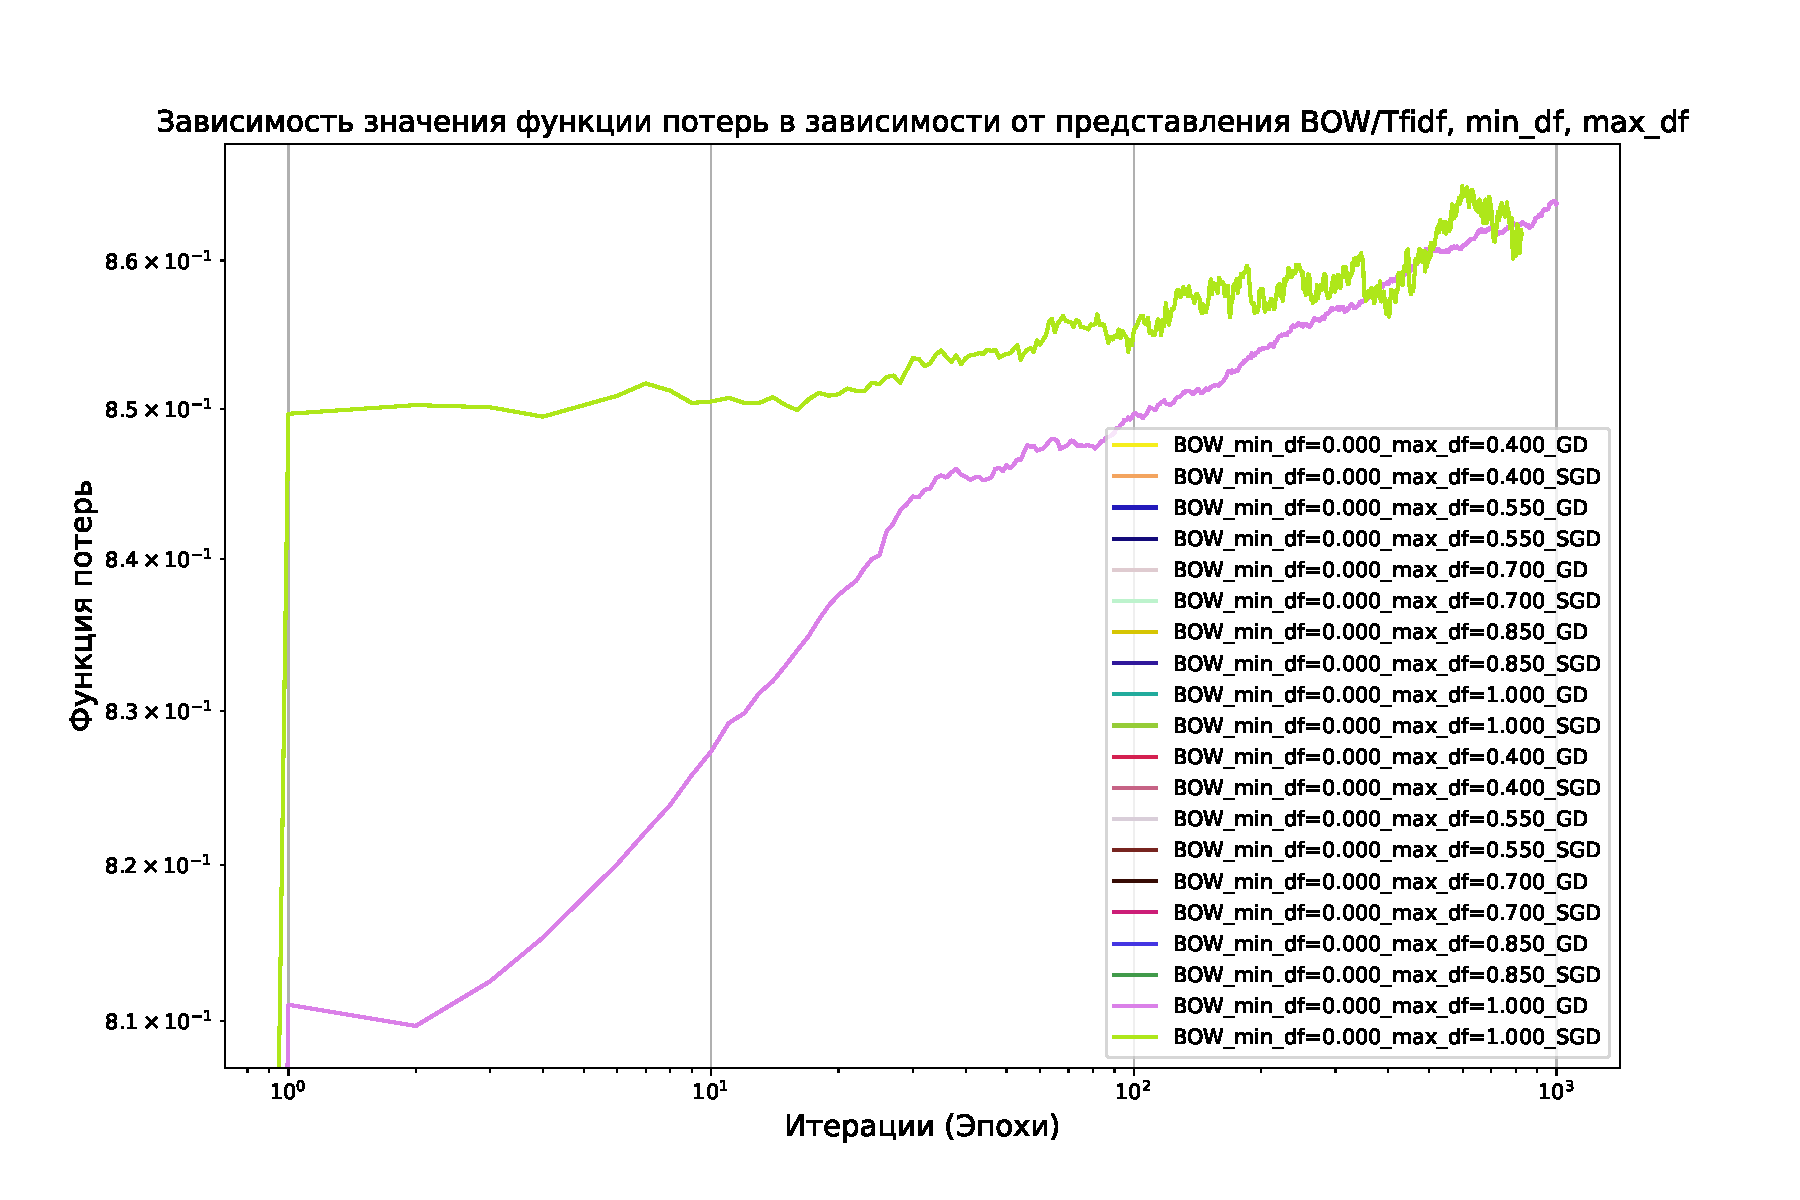
\includegraphics[width=0.85\linewidth]
    {exp_8_min_max_df_loss_1.pdf}
    \caption{Значения функции потерь на итерациях (эпохах) методов GD/SGD в зависимости от представления \textit{BOW/Tfidf} и параметров \textit{min\_df} и \textit{max\_df}}
    \label{fig:exp_8_min_max_df_loss_1}
\end{figure}

\begin{figure}[H]
    \centering
    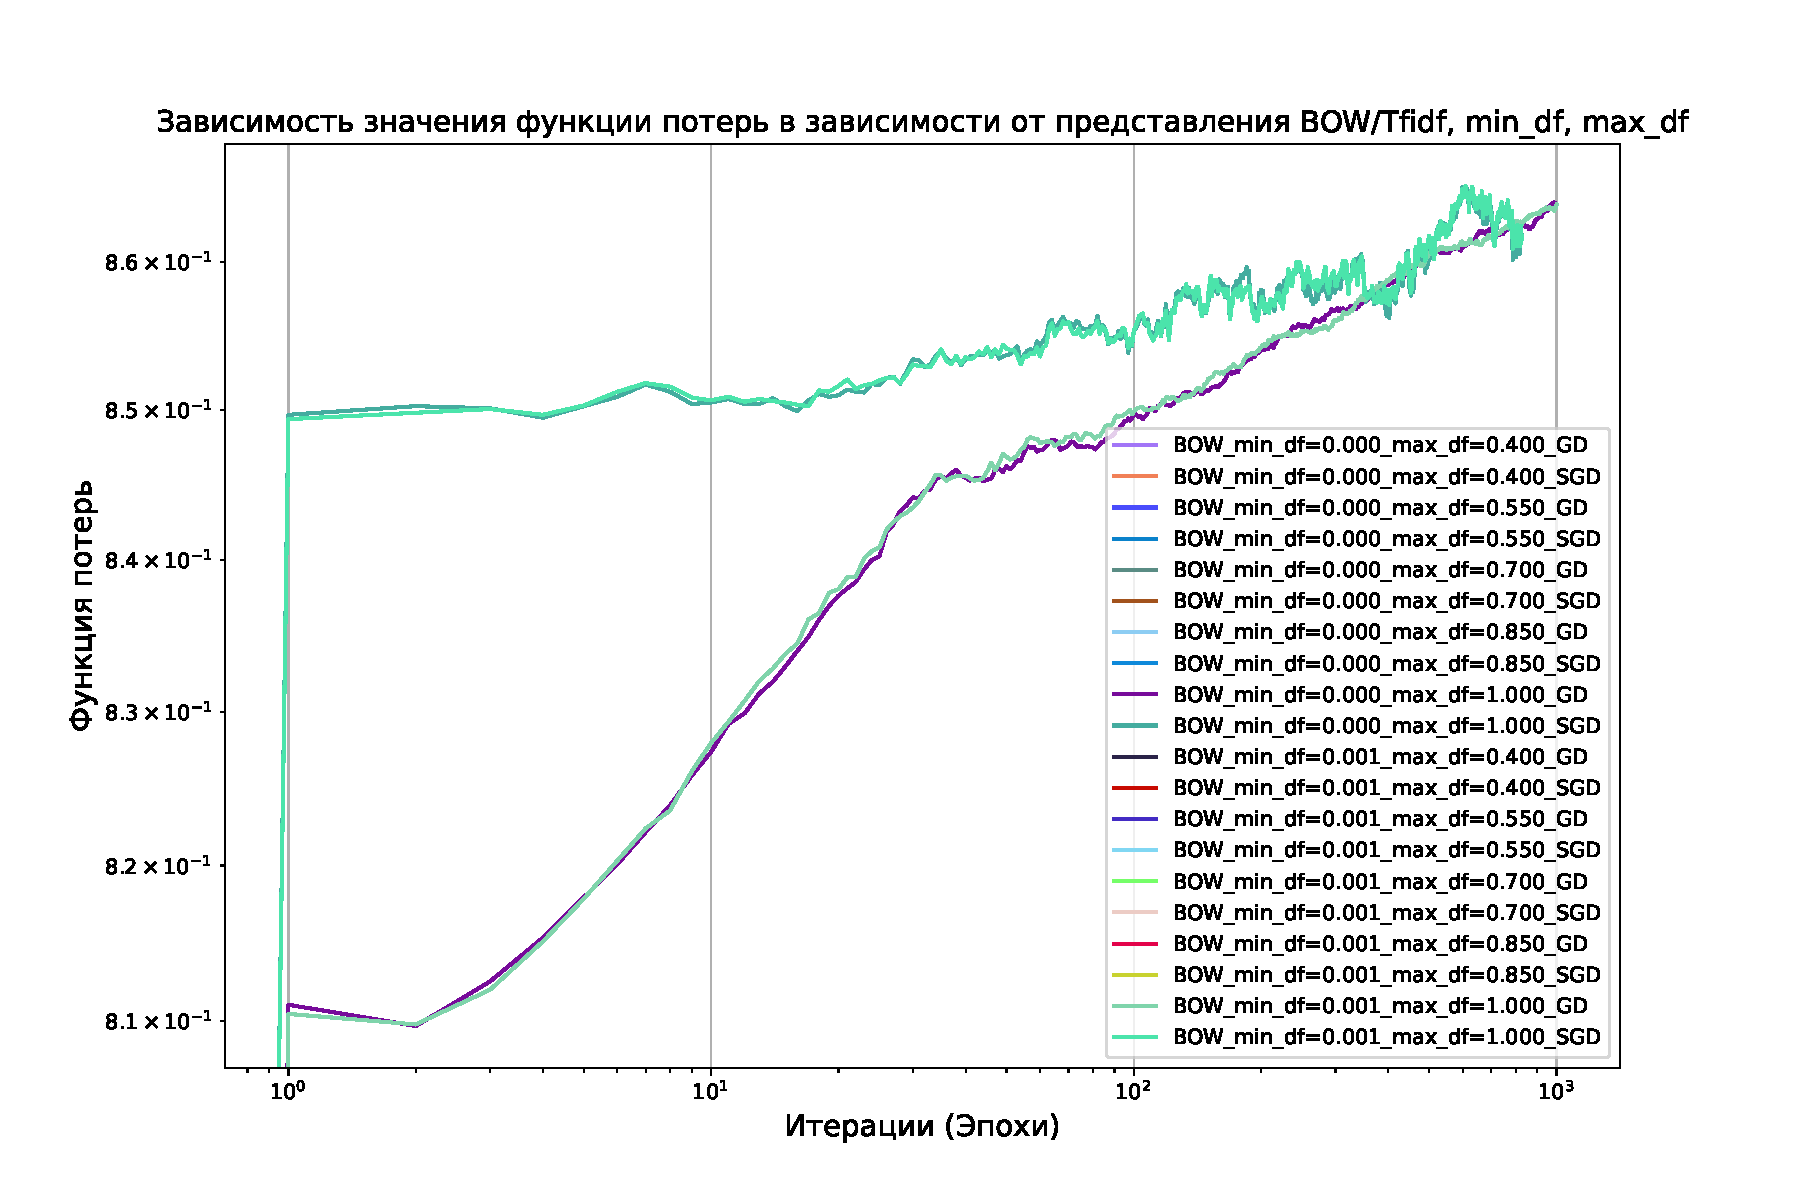
\includegraphics[width=0.85\linewidth]
    {exp_8_min_max_df_loss_2.pdf}
    \caption{Значения функции потерь на итерациях (эпохах) методов GD/SGD в зависимости от представления \textit{BOW/Tfidf} и параметров \textit{min\_df} и \textit{max\_df}}
    \label{fig:exp_8_min_max_df_loss_2}
\end{figure}

\begin{figure}[H]
    \centering
    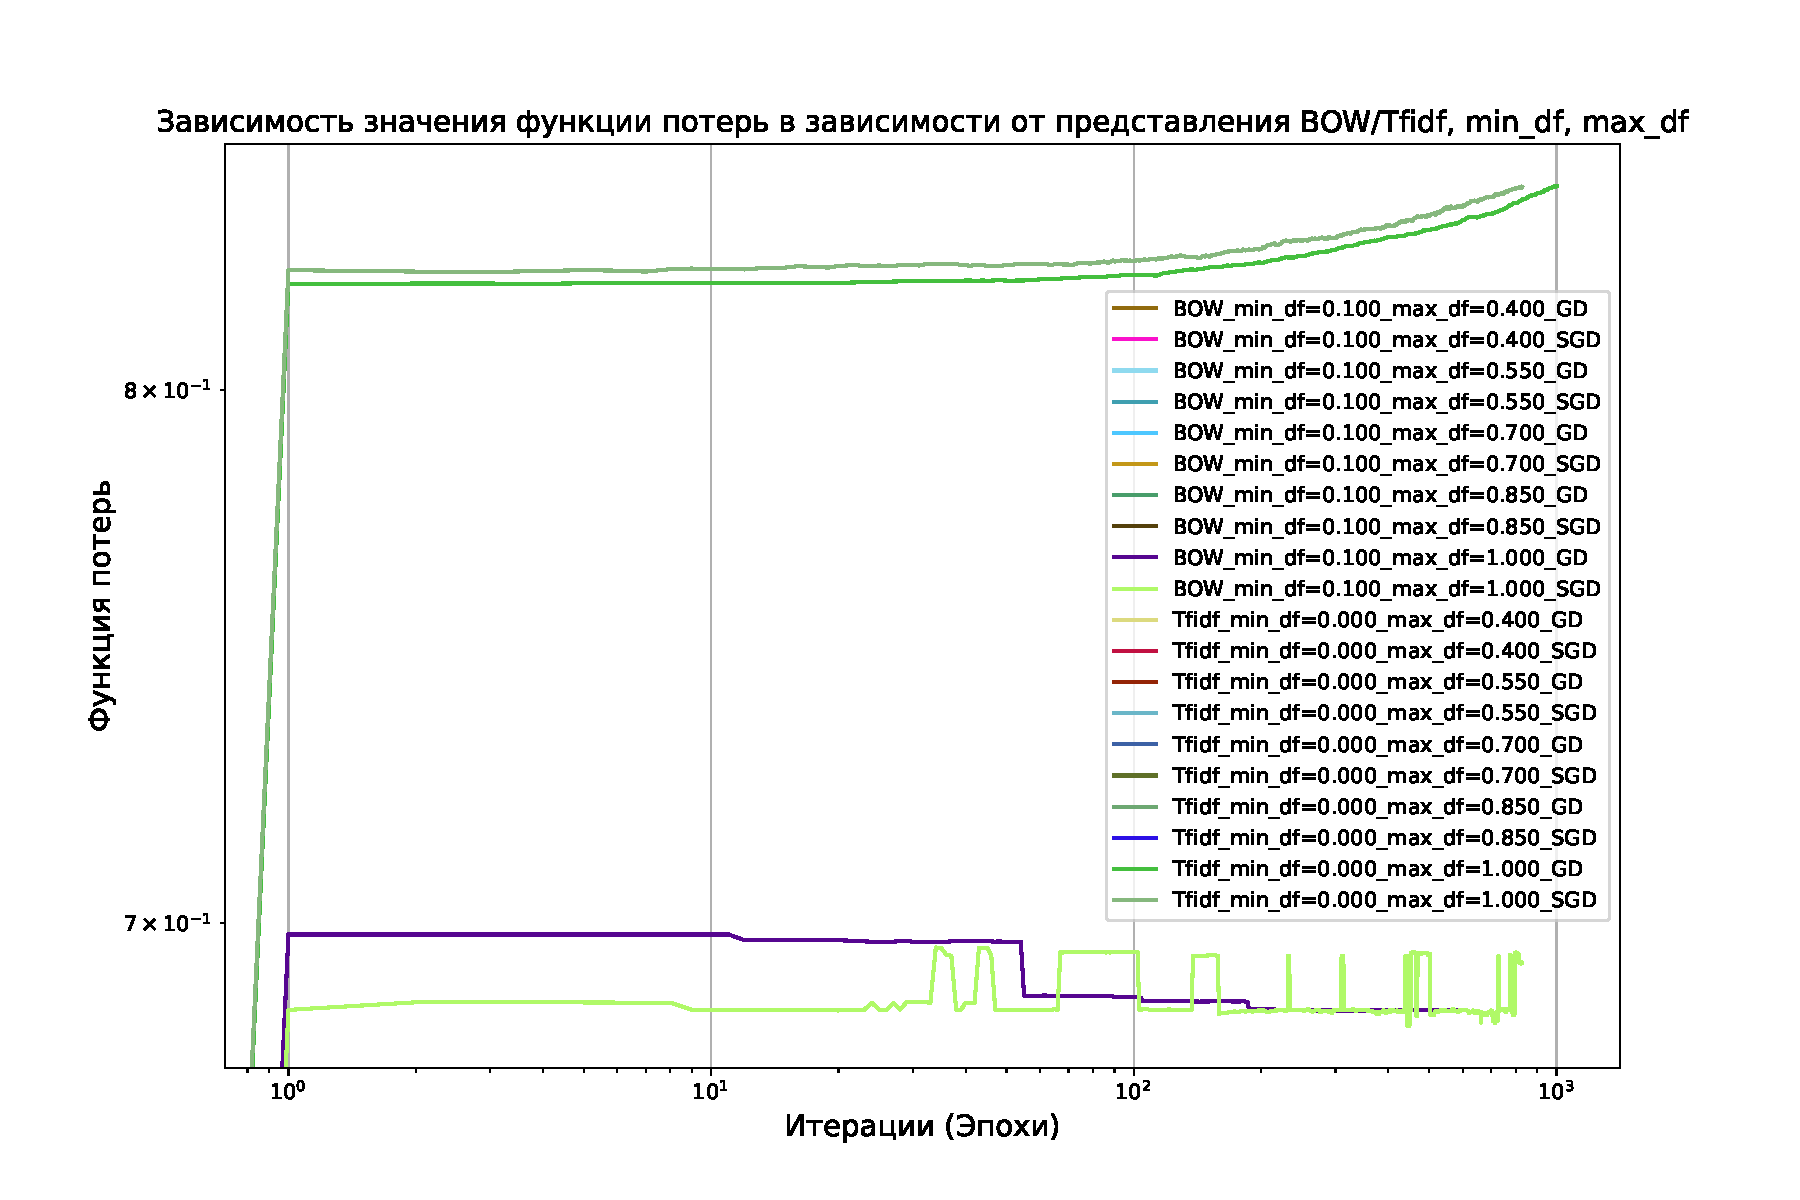
\includegraphics[width=0.85\linewidth]
    {exp_8_min_max_df_loss_3.pdf}
    \caption{Значения функции потерь на итерациях (эпохах) методов GD/SGD в зависимости от представления \textit{BOW/Tfidf} и параметров \textit{min\_df} и \textit{max\_df}}
    \label{fig:exp_8_min_max_df_loss_3}
\end{figure}

\begin{figure}[H]
    \centering
    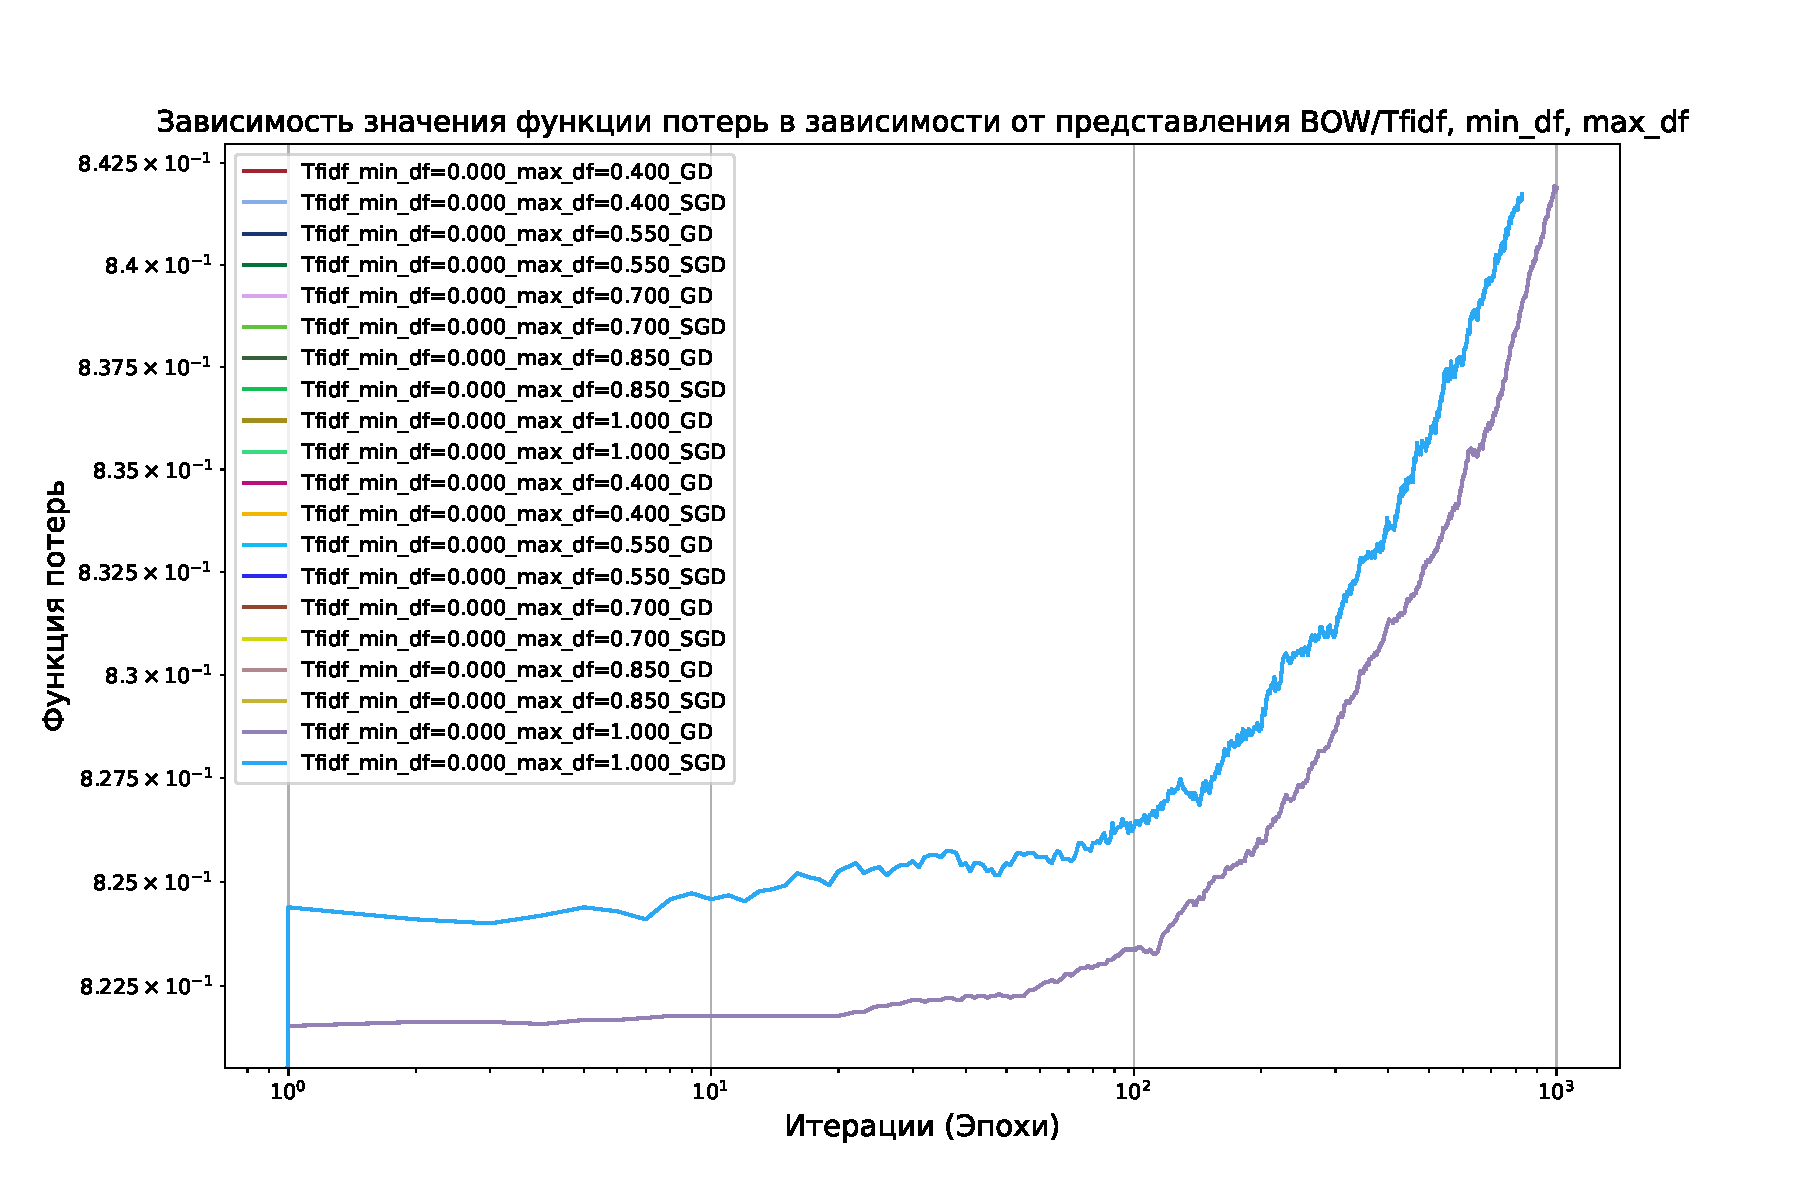
\includegraphics[width=0.85\linewidth]
    {exp_8_min_max_df_loss_4.pdf}
    \caption{Значения функции потерь на итерациях (эпохах) методов GD/SGD в зависимости от представления \textit{BOW/Tfidf} и параметров \textit{min\_df} и \textit{max\_df}}
    \label{fig:exp_8_min_max_df_loss_4}
\end{figure}

\begin{figure}[H]
    \centering
    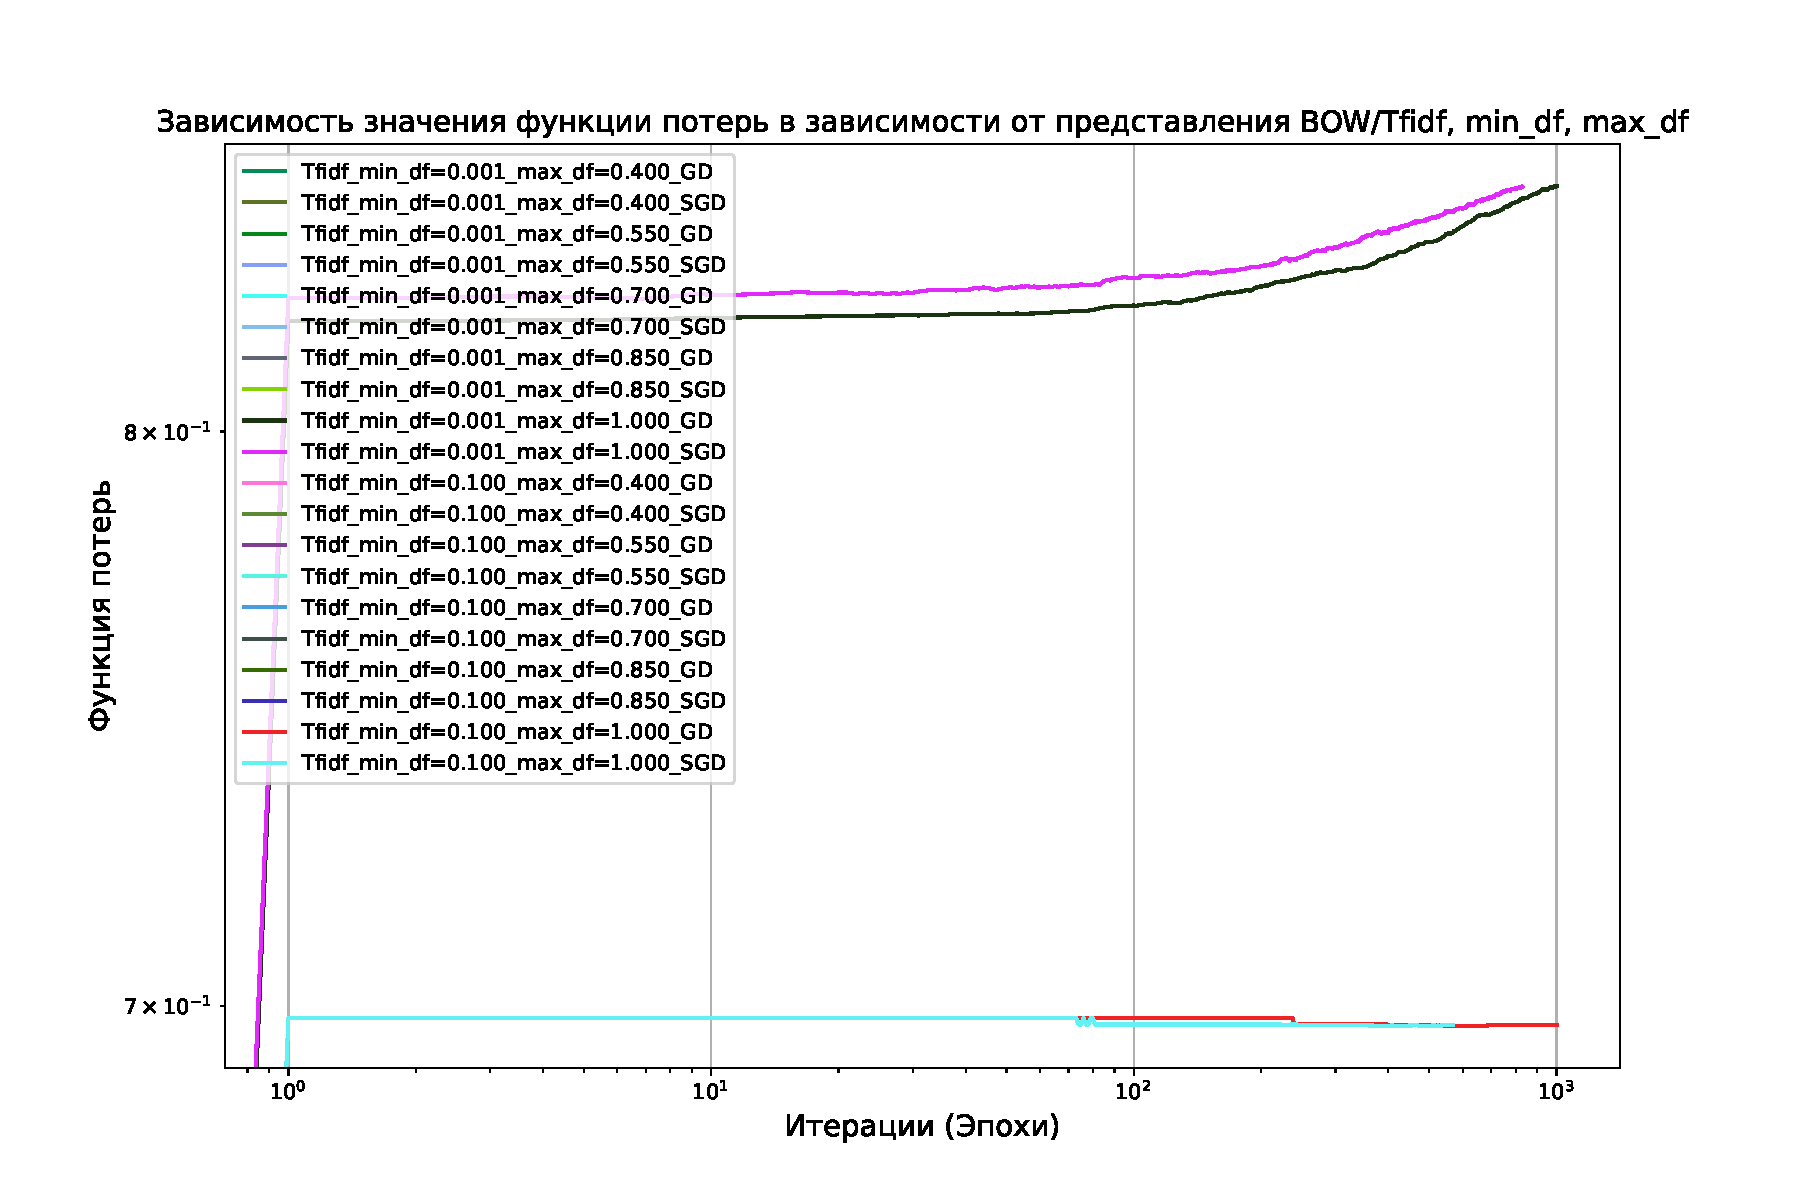
\includegraphics[width=0.85\linewidth]
    {exp_8_min_max_df_loss_5.pdf}
    \caption{Значения функции потерь на итерациях (эпохах) методов GD/SGD в зависимости от представления \textit{BOW/Tfidf} и параметров \textit{min\_df} и \textit{max\_df}}
    \label{fig:exp_8_min_max_df_loss_5}
\end{figure}

На рисунках \hyperref[fig:exp_8_min_max_df_loss_1]{46}, \hyperref[fig:exp_8_min_max_df_loss_2]{47}, \hyperref[fig:exp_8_min_max_df_loss_3]{48}, \hyperref[fig:exp_8_min_max_df_loss_4]{49}, \hyperref[fig:exp_8_min_max_df_loss_5]{50}  представлены графики зависимости значения функции потерь на каждой итерации (эпохе) градиентного и стохастического градиентного спуска от представления \textit{BOW/Tfidf} и параметров \textit{min\_df} и \textit{max\_df}.

Проанализируем размерность признакового пространства выборки в зависимости от параметров \textit{min\_df} и \textit{max\_df}.

\begin{figure}[H]
    \centering
    \includegraphics[width=0.85\linewidth]
    {exp_8_min_max_df_size.pdf}
    \caption{Зависимости размерность признакового пространства выборки от параметров \textit{min\_df} и \textit{max\_df}}
    \label{fig:exp_8_min_max_df_size}
\end{figure}

На рисунке \hyperref[fig:exp_8_min_max_df_size]{51} представлен график зависимости размерности признакового пространства выборки от параметров \textit{min\_df} и \textit{max\_df}. Как можно заметить из графика, сильное уменьшение \textit{max\_df} или сильное увеличение \textit{min\_df} приводит к слишком большой размерности сокращению признакового пространства, а сильное увеличение \textit{max\_df} или сильное уменьшение \textit{min\_df} - к слишком большой размерности признакового пространства.

\subsection{Выводы}

Рассмотрим распределение времени выполнения одного метода и accuracy (\hyperref[fig:exp_8_min_max_df_time_acc_raspred]{См. рис. 52}) для определения наиболее оптимальных представления и параметров:

\begin{figure}[ht]
    \centering
    \begin{subfigure}{0.48\textwidth}
        \centering
        \includegraphics[width=\linewidth]
        {exp_8_min_max_df_time_raspred.pdf}
        \caption{Распределение времени выполнения}
        \label{fig:exp_8_min_max_df_time_raspred}
    \end{subfigure}
    \hspace{-0.5em}
    \begin{subfigure}{0.48\textwidth}
        \centering
        \includegraphics[width=\linewidth]
        {exp_8_min_max_df_acc_raspred.pdf}
        \caption{Распределение accuracy}
        \label{fig:image2}
    \end{subfigure}
    \caption{Распределения времени выполнения и accuracy для методов, обученных на различных представлениях \textit{BOW/Tfidf} и параметрах \textit{min\_df} и \textit{max\_df}}
    \label{fig:exp_8_min_max_df_time_acc_raspred}
\end{figure}

Выберем те модели, которые выполняются быстрее 10 секунд, имеют точность больше 0.86 и размер признакового пространства выборки, на которой обучалась модель больше 100, но меньше 7000 (\hyperref[tab:exp_8_models_best]{См. табл. 5}):


\begin{table}[H]
    \centering
    \begin{tabular}{|c|c|c|c|c|c|c|}
        \hline
        model & repres & min\_df & max\_df & accuracy & X.shape[1] & time \\ \hline
        \textit{SGD} & \textit{BOW} & 0.000562 & 0.40 & 0.86153 & 4724 & 7.022379 \\ \hline
        \textit{SGD} & \textit{BOW} & 0.000562 & 0.55 & 0.86153 & 4724 & 7.479241 \\ \hline
        \textit{SGD} & \textit{BOW} & 0.000562 & 0.70 & 0.86153 & 4724 & 7.314365 \\ \hline
        \textit{SGD} & \textit{BOW} & 0.000562 & 0.85 & 0.86153 & 4724 & 7.462992 \\ \hline
        \textit{SGD} & \textit{BOW} & 0.000562 & 1.00 & 0.86153 & 4724 & 7.316502 \\ \hline
    \end{tabular}
    \caption{Модели, соответствующие параметрам}
    \label{tab:exp_8_models_best}
\end{table}

Выберем наилучшие параметры и представление, основываясь на балансе скорости работы и точности.

Таким образом, наилучшими будут:
\begin{itemize}
    \item Представление  - \textit{BOW}
    \item \textit{min\_df} - 0.000562
    \item \textit{max\_df} - 0.7
\end{itemize}

\section{Выбор лучшего алгоритма и анализ ошибок}

\subsection{Постановка задачи}

\begin{itemize}
    \item Выбрать лучший алгоритм для тестовой выборки.
    \item Проанализировать ошибки алгоритма.
    \item  Проанализировать и указать общие черты объектов, на которых были допущены ошибки.
\end{itemize}

\subsection{Реализация}

\subsubsection{Создание лучшей модели}

На основании проведённого анализа в предыдущих пунктах можно сделать вывод, что модель стохастического градиентного спуска уступает методу градиентного спуска по точности (accuracy), но значительно превосходит его по скорости работы. В связи с этим, обучим модель SGD с использованием ранее определённых оптимальных параметров, а также с применением лемматизации выборки и представления данных, параметры которого также были выбраны как наилучшие в ходе анализа. Хотя предложенная модель может уступать градиентному спуску по точности, она будет демонстрировать значительное преимущество в скорости работы.

Лучшие параметры и представления, полученные ранее:
\begin{itemize}
    \item \textit{step\_alpha = 3.72759372e-01}
    \item \textit{step\_beta = 0.001}
    \item \textit{$w_0 = (0, ... , 0)$} 
    \item \textit{batch\_size = 300}
    \item \textit{l2\_coef = 0.00183298071}
    \item представление - \textit{BagOfWords}
    \item параметр конструктора представления \textit{min\_df = 0.000562}
    \item параметр конструктора представления \textit{max\_df = 0.7}
\end{itemize}

Ниже приведено время обучения данной модели и accuracy на тестовой выборке (\hyperref[tab:exp_9_best_model_acc_time]{см. табл. 6}), а также графики зависимости accuracy и значения функции потерь от эпохи метода  (см. рис. \hyperref[fig:exp_9_acc]{53} и \hyperref[fig:exp_9_loss]{54}):

\begin{table}[H]
    \centering
    \begin{tabular}{|c|c|}
        \hline
        Accuracy & Время обучения модели(сек.) \\ \hline
        0.8626910427548848 & 11.371453762054443 \\ \hline
    \end{tabular}
    \caption{Точность на тестовой выборке и время обучения лучшей модели}
    \label{tab:exp_9_best_model_acc_time}
\end{table}

\begin{figure}[H]
    \centering
    \includegraphics[width=0.85\linewidth]
    {exp_9_acc.pdf}
    \caption{Зависимость accuracy от эпохи получившегося метода}
    \label{fig:exp_9_acc}
\end{figure}

\begin{figure}[H]
    \centering
    \includegraphics[width=0.85\linewidth]
    {exp_9_loss.pdf}
    \caption{Зависимость значения функции потерь от эпохи получившегося метода}
    \label{fig:exp_9_loss}
\end{figure}

\subsubsection{Анализ ошибок}

Для анализа ошибок нашей модели построим матрицу ошибок (\hyperref[fig:exp_9_conf_matrix]{См. рис. 55}):

\begin{figure}[H]
    \centering
    \includegraphics[width=0.85\linewidth]
    {exp_9_conf_matrix_fixed.pdf}
    \caption{Матрица ошибок алгоритма}
    \label{fig:exp_9_conf_matrix}
\end{figure}

Ложно положительных объектов - 1936, ложно отрицательных - 903. \\

Проанализируем ошибки на примерах: \\
\begin{itemize}
 \item False Negative объекты:
\begin{itemize}
    \item \begin{quote} uncivil b ignorance persistence think saying correct already provoking provoking already act incivility offence idiot would given talking oh ironic still talk page afraid willing discus anything future well nice feel exact way halleluiah agreement something lol hope weird see said ton time one deluded people think right time whenever proved otherwise shutdown try turn table person wrong uncivil \end{quote}
    \item \begin{quote} pigsonthewing pigsonthewing aka andy mabbett obese stink booze need wear bikini often thanks leonig mig \end{quote}
    \item \begin{quote} hey kendricks pittsburgh compton wack motherfucker nwa would ashamed boyyyyyyyyyyyyyyy \end{quote}
    \item \begin{quote} barnstar thanks barnstar big sexy pimp \end{quote}
    \item \begin{quote} see left part supposed discussing quickly reverted shabazz wrongly claimed done good deleting certainly anyone honest non biased situation would disagree merely placed paragraph question different area trimmed bit unless someone determined make paragraph important action jidf claiming statement something bad deleting would true therefore feel hostile intention concerned people respect feel good intention ganging handle also thinking since shabazz essentially told get lost think going stick around get louder also going get many friend respect noble intention start getting involved f ridiculous \end{quote}
    \item \begin{quote} sick idiocy going de watchlist whole lot ai article never ending pointless battle fancruft always win good riddance \end{quote}
    \item \begin{quote} dumbass called also responsible \end{quote}
    \item \begin{quote} user page please stop putting crap thanks \end{quote}
    \item \begin{quote} support merge sucker \end{quote}
    \item \begin{quote} lake bob would someone please stop changing reference lake bob farris sea care name referenced old news article simply called current student personally attest fact universally called lake bob student faculty alike also would whatever student responsible recent vandalism please quit wikipedia place play stupid prank air grudge school end making look like fool thanks \end{quote}
\end{itemize}


\item False Positive объекты:
\begin{itemize}
    \item \begin{quote} know get around watching soon know seen punk stuff reason really really annoys know good wrestler like oh get started wwe treatment paul london seen load indy work stuff roh amazing fucking awesome wwe fucked big time went arounf rumor site got released planning quitting wrestling moving acting something would suck stupid wwe penchant asshole look like steroid like cena idiot like batista bitched moved raw got beat jericho title take deep breath sorry ranting \end{quote}
    \item \begin{quote} enjoy stay \end{quote}
    \item \begin{quote} brainloss swedish word hj rnsl pp loosely translated brainloss braindrop brain drop head meaning feeling get realise act utter stupidity done even understand could stupid tagging article deletion wrong title moved different title good thing resourceful brain dept \end{quote}
    \item \begin{quote} posted sharon mooney \end{quote}
    \item \begin{quote} teacher really dumb people think people first last name people mr williams teacher \end{quote}
    \item \begin{quote} nice attempt look horrible crammed way much information small as area honestly fix far lazy \end{quote}
    \item \begin{quote} care people caring read one care coming either treelo going hire lawyer either sued dare delete message message give period edt \end{quote}
    \item \begin{quote} support someone calling stupid registered editor nice know please give warning deserve \end{quote}
    \item \begin{quote} spell kris draper without kid raper \end{quote}
    \item \begin{quote} die teutsche wikipedia ist voll von menschen wie ihnen einer mehr macht allerdings auch nichts au \end{quote}
\end{itemize}
\end{itemize}

\subsection{Выводы}
\begin{itemize}
    \item Построен лучший алгоритм по ранее определенным оптимальным параметрам с точностью, равной  \textit{0.8626910427548848}, и временем работы \textit{11.371453762054443} секунд.
    \item Ошибки False Negative связаны с неспособностью модели обнаруживать скрытую токсичность, сарказм или пассивно-агрессивные высказывания. Такие комментарии часто содержат оскорбительные слова, но иногда токсичность проявляется на уровне подтекста или скрытой агрессии, что требует более сложного анализа контекста. Кроме того, грамматические ошибки и нестандартные синтаксические конструкции в тексте могут приводить к тому, что модель не распознает явную токсичность. Сложные многосоставные предложения также затрудняют правильную интерпретацию комментария. В случае False Positive, где нетоксичные комментарии классифицируются как токсичные, проблемы возникают из-за эмоциональной окраски текста, использования сложных слов с потенциально двойным смыслом, а также из-за нейтральной критики, которая может быть ошибочно воспринята как токсичная. Модель также может неверно интерпретировать фразы на других языках или сложные конструктивные комментарии, которые содержат отдельные слова, ошибочно распознаваемые как токсичные. \\ Таким образом, основными проблемами являются трудности в учёте контекста, распознавании скрытой токсичности и правильной интерпретации эмоционально окрашенных текстов.
\end{itemize}


\section{Итог}

В ходе выполнения работы проведен анализ линейных моделей на примере задачи классификации токсичности комментариев. Реализованы методы градиентного и стохастического градиентного спуска, проведено их сравнение с учетом различных параметров, таких как размер шага, начальное приближение весов, размер подвыборки и коэффициент регуляризации. Выявлено, что градиентный спуск показывает немного более высокую точность, но стохастический градиентный спуск значительно превосходит его по скорости работы. Лемматизация данных продемонстрировала улучшение точности обоих методов за счет сокращения размерности признакового пространства, хотя и увеличила общее время выполнения алгоритмов.

Также выполнено сравнение различных представлений данных — \textit{BagOfWords} и \textit{Tfidf}. Представление \textit{BagOfWords} оказалось более точным, однако \textit{Tfidf} обеспечило более быстрое выполнение задач.

В рамках анализа ошибок алгоритма было установлено, что модель иногда ошибается на комментариях с сарказмом, скрытой агрессией и нетипичными синтаксическими конструкциями, что связано с ограничениями выбранных моделей.

Также, был составлен лучший алгоритм по ранее определенным оптимальным параметрам с точностью, равной  \textit{0.8627}, и временем работы \textit{11.3715} секунд.

Таким образом, лучшие результаты по точности достигнуты с использованием метода градиентного спуска, лемматизации и представления \textit{BagOfWords}. В то же время, стохастический градиентный спуск с представлением TF-IDF является более эффективным выбором для задач, требующих быстродействия.

\begin{thebibliography}{9}
\bibitem{voron} Материалы семинаров ММРО и Практикума 3 курса ВМК МГУ, \url{https://github.com/mmp-practicum-team/mmp_practicum_fall_2024/blob/main/Seminars/08-text-processing-and-logreg/seminar.pdf}
\bibitem{voron} kaggle, \url{https://www.kaggle.com/c/jigsaw-toxic-comment-classification-challenge\models}
\end{thebibliography}


\end{document}